\newcommand{\ttbar}{$\textrm{t}\bar{\textrm{t}}~$}
\newcommand{\bbbar}{$\textrm{b}\bar{\textrm{b}}~$}
\newcommand{\ptmiss}{$p_{T}^{\mathrm{miss}}~$}

\chapter{Search for physics beyond the Standard Model using boosted H bosons and missing transverse momentum in proton-proton collisions at 13 TeV}
\label{chap:analysis}

\section{Motivation \& Strategy}

If a more unifying theory than the SM exists it certainly has not been forthright in its manifestation. One possibility for the lack of discoveries of phenomena not explained within the SM is that there are indeed particles existing in Nature which have not been observed, but they have such a large mass the energy of the proton-proton collisions provided by the LHC is insufficient to directly create them. The outcome of many searches for new particles is thus the setting of lower limits placed on the mass -- if the particle were any lighter than this limit it would have been produced copiously enough for its unambiguous detection (see for example \cite{CMS-SUS-16-033, CMS-SUS-15-002}). As these particles become more massive more momentum is imparted upon the particles involved in the final state; any SM particles resulting from the decay of higher mass states will be produced with large momentum (this is called high boost). As a particle becomes more boosted its decay products are emitted at smaller angles, eventually collimating sufficiently to be reconstructed as a single jet. If new physics exists with masses achievable by the LHC, one could suspect that there exists non-zero coupling with the electroweak H, Z, or W bosons. Observation of events containing high-$p_{T}$ ($>$300 GeV) electroweak bosons are thus of considerable interest for some hints of something unseen.

The Minimal Supersymmetric SM contains a $\mathbb{Z}_{2}$ symmetry in which all SM particles have charge -1 and all supersymmetric particles have charge +1, this is called R-parity \cite{susyprimer}. One direct consequence of R-parity is that the decay of a massive supersymmetric particle must include at least one supersymmetric particle in the final state. Necessarily this is the lightest such particle in the theory, denoted the lightest supersymmetric particle (LSP). If the LSP is electrically neutral it may escape detection, creating an imbalance in the net momentum of the event (as would a neutrino). Events with a large momentum imbalance are also interesting as potential regions for SUSY.

With this as motivation, we designed an analysis searching for hints of new physics beyond the SM in events with boosted H or Z bosons and a large transverse momentum imbalance of the event. We reconstruct the H and Z bosons in the $b\bar{b}$ channel, with 57\% and 15\% branching fractions respectively. Although our analysis is sensitive to any new physics with this final state, we have adopted two benchmark models (known as SMS models \cite{CMS-SUS-11-016} - phenomenological models of SUSY at hadron colliders), seen in Figure~\ref{fig:sms}, to give motivation to the analysis. In this scenario, the proton-proton interaction produces a pair of gluinos $\tilde{g}$ (the blob in the figure indicates we are not interested in the particulars of the gluino production mechanism) which decay to a neutralino $\tilde{\chi}_{2}^{0}$ by the emission of SM quarks. A small mass splitting between the gluino $\tilde{g}$ and neutralino $\tilde{\chi}_{2}^{0}$ will result in low-$p_{T}$ SM quarks and a high-$p_{T}$ neutralino $\tilde{\chi}_{2}^{0}$. This neutralino $\tilde{\chi}_{2}^{0}$ further decays into neutralino $\tilde{\chi}_{1}^{0}$ with the emission of a H or Z boson. The neutralino $\tilde{\chi}_{1}^{0}$ is the LSP and escapes detection. 
 
Past searches targeting similar final states (but different production scenario, i.e. another SMS model) have been performed in which the H bosons are produced with low-$p_{T}$, in this case the H bosons are reconstructed as a resolved pair of b-tagged AK4 jets \cite{CMS-SUS-16-044}.
 
\begin{figure}[hbp!]
\centering
\begin{subfigure}[b]{0.425\textwidth}
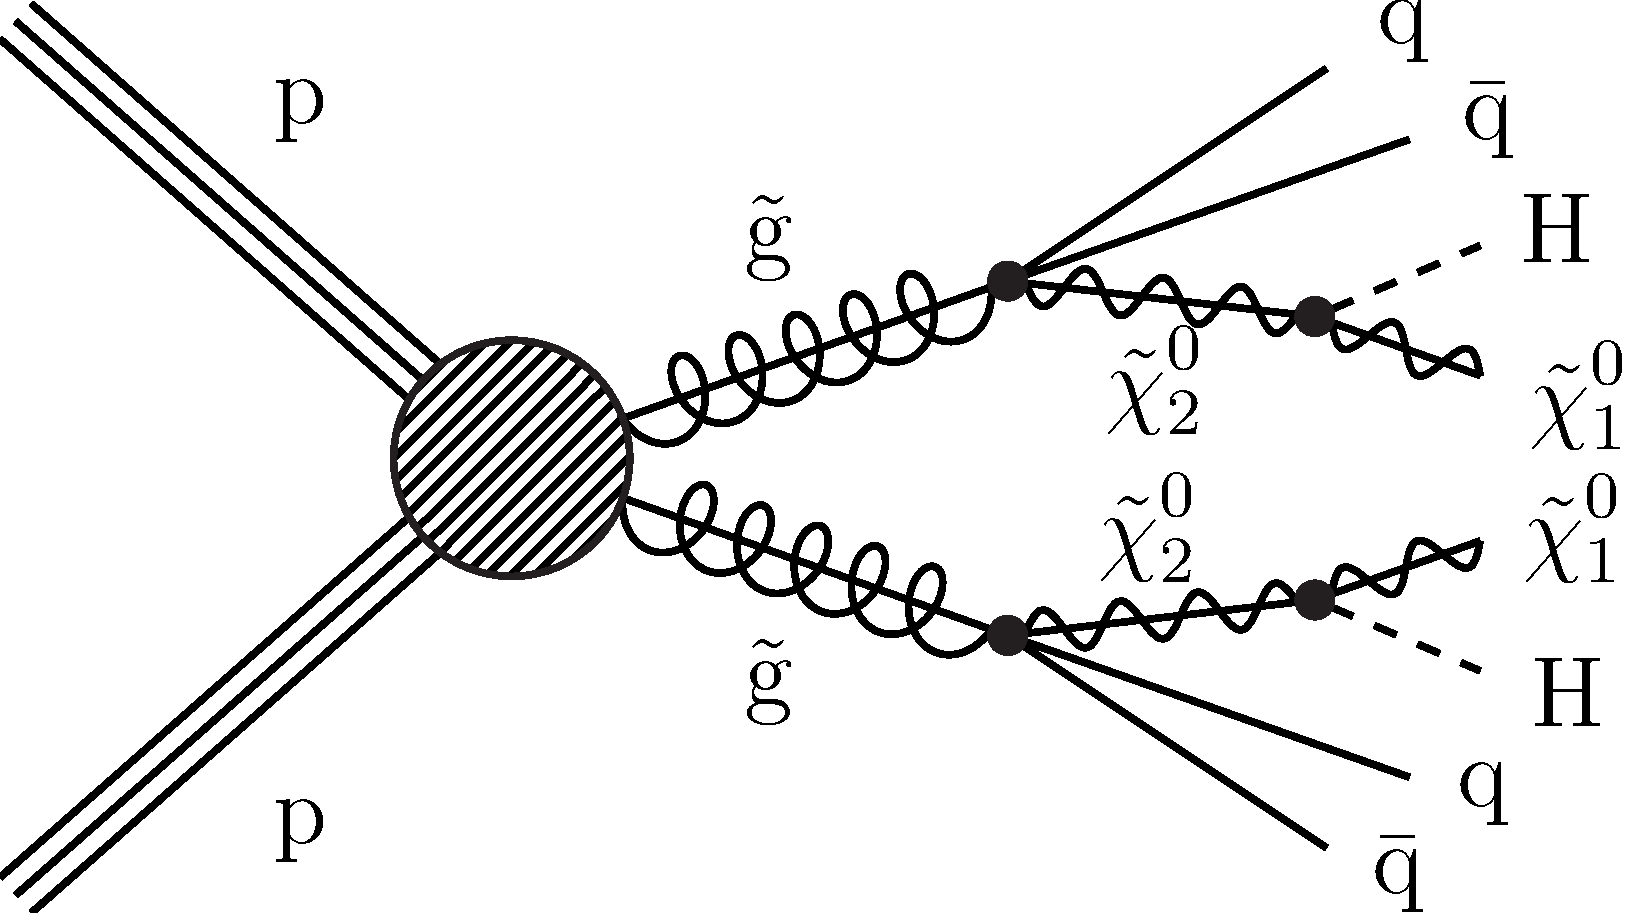
\includegraphics[width=0.95\textwidth]{figs/CMS-SUS-17-006_Figure_001.pdf}
\caption{The T5HH SMS model.}
\label{fig:t5hh}
\end{subfigure}
\begin{subfigure}[b]{0.425\textwidth}
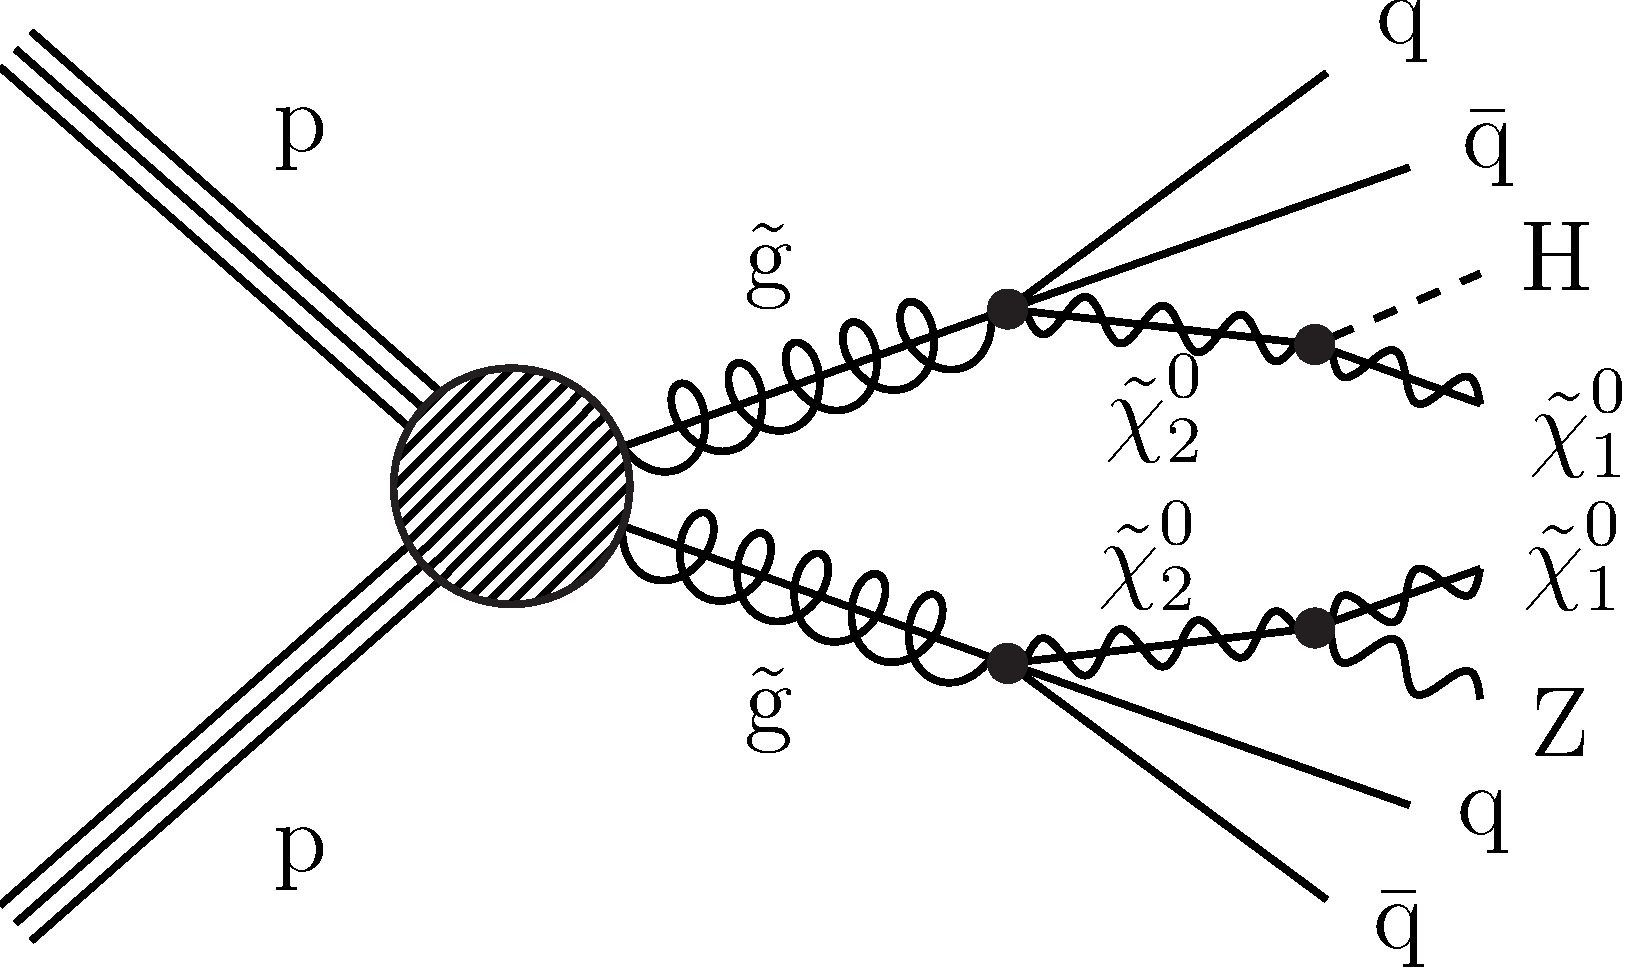
\includegraphics[width=0.95\textwidth]{figs/CMS-SUS-17-006_Figure-aux_001.pdf}
\caption{The T5ZH SMS model.}
\end{subfigure}
\caption{Diagrams of the benchmark models used for motivation of the targeted signal.}
\label{fig:sms}
\end{figure}

\section{Object Definition \& Event Selection}

We establish a baseline selection choosing events with all-hadronic final states and missing transverse momentum (\ptmiss), as motivated by Figure~\ref{fig:sms}. The baseline selection is as follows:

\begin{itemize}
\item $\geq2$ AK8 jets; $p_{T} > 300\,\mathrm{GeV}$ and $50 < \mathrm{mass} < 250\,\mathrm{GeV}$
\item $p_{T}^{\mathrm{miss}} > 300\,\mathrm{GeV}$;
\item isolated electron veto; $p_{T}>10\,\mathrm{GeV}$\newline
To remove events with top or W production in which the W decays to an electron.
\item isolated muon veto; $p_{T}>10\,\mathrm{GeV}$\newline
To remove events with top or W production in which the W decays to a muon.
\item isolated track veto\newline
To remove events with top or W production in which the W decays to a tau. The tau branching fraction to states containing at least one charged particle is 85\%. As an isolated track is defined by looser criteria than that of an electron or muon, this cut also serves to increase the efficiency of the isolated electron and muon vetoes.

\item $\Delta\phi_{1, 2, 3, 4} > 0.5, 0.5, 0.3, 0.3$; $\Delta\phi_{i}\equiv \Delta\phi(\vec{p_{T}}^{\mathrm{miss}}, \mathrm{AK4\,jet}_{i})$\newline
The $\Delta\phi$ cut is designed to mitigate QCD events in which a jet is under-measured leading to an artificial imbalance in the event momentum. This cut requires that the difference in $\phi$ between the \ptmiss vector and each of the four leading AK4 jets is sufficiently large to remove events in which a jet has been under-measured giving rise to fake \ptmiss pointing in the same direction. If less than four AK4 jets are available the additional cuts are removed.
\end{itemize}

A dedicated heavy tagging algorithm is used to identify AK8 jets arising from the decay of two b quarks \cite{bbtagger}. The distribution of the output discriminator for the lead and sub-leading jets are seen in the left and right panels of Figure~\ref{fig:ak8dists}, respectively; signal-like events peak towards larger values. To $b\bar{b}$ tag the AK8 jets we choose the loose working-point ($>$0.3) corresponding to a signal efficiency of approximately $80\%$ per AK8 jet (see Section~\ref{sec:reinterpretation}). The stacked histogram and solid lines shows the distribution after baseline selection for simulation and two representative signal points, respectively.

Further H/Z tagging of an AK8 jet is accomplished by restricting the jet mass window to [85, 135 GeV] to be consistent with that of the H boson. The distributions of the jet mass are seen in Figure~\ref{fig:ak8dists}. The signal shown in the solid line is the T5HH model (i.e. Figure~\ref{fig:t5hh}). The same identification criteria are applied to tag an AK8 jet as either an H or Z boson, there is no distinction made.

\begin{figure}[hbp!]
\centering
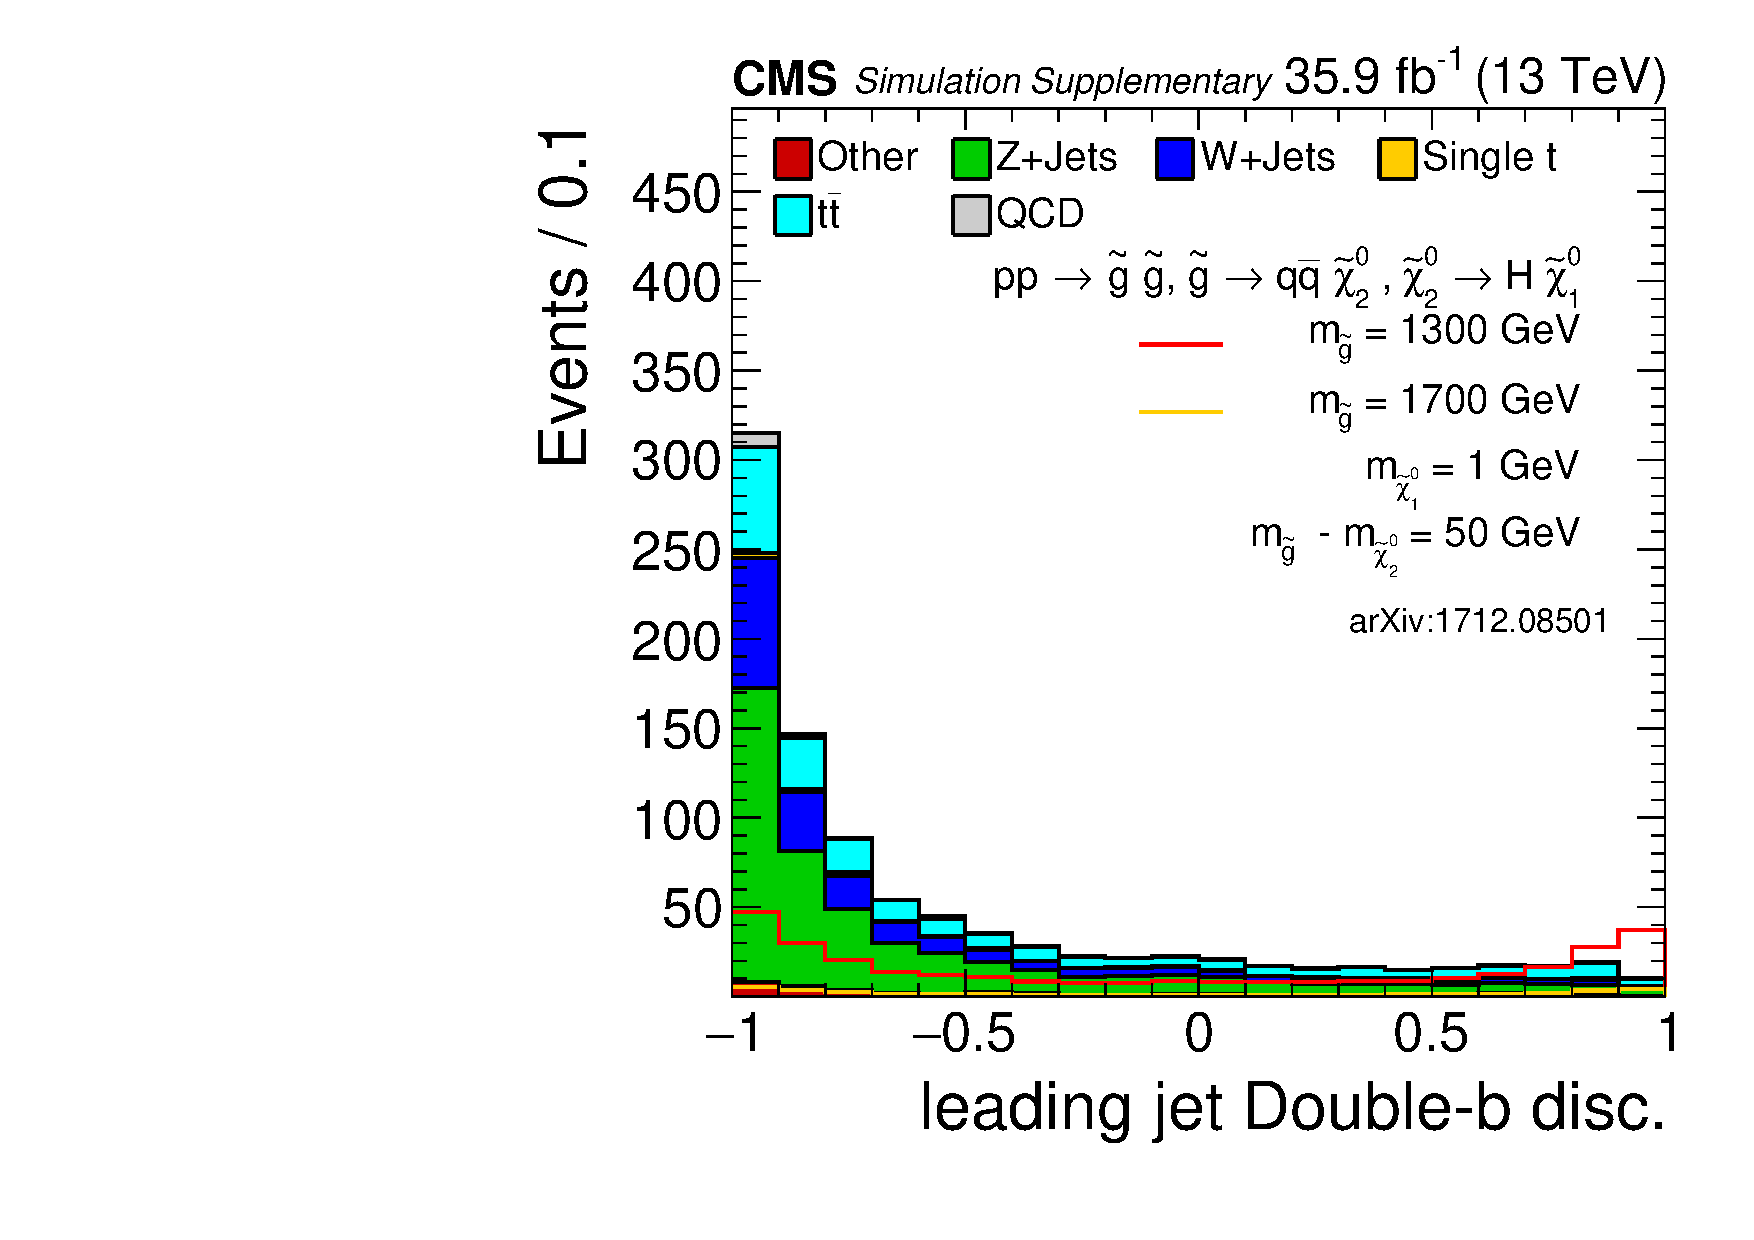
\includegraphics[width=0.425\linewidth]{figs/J1BB_LooseJetMass.pdf}
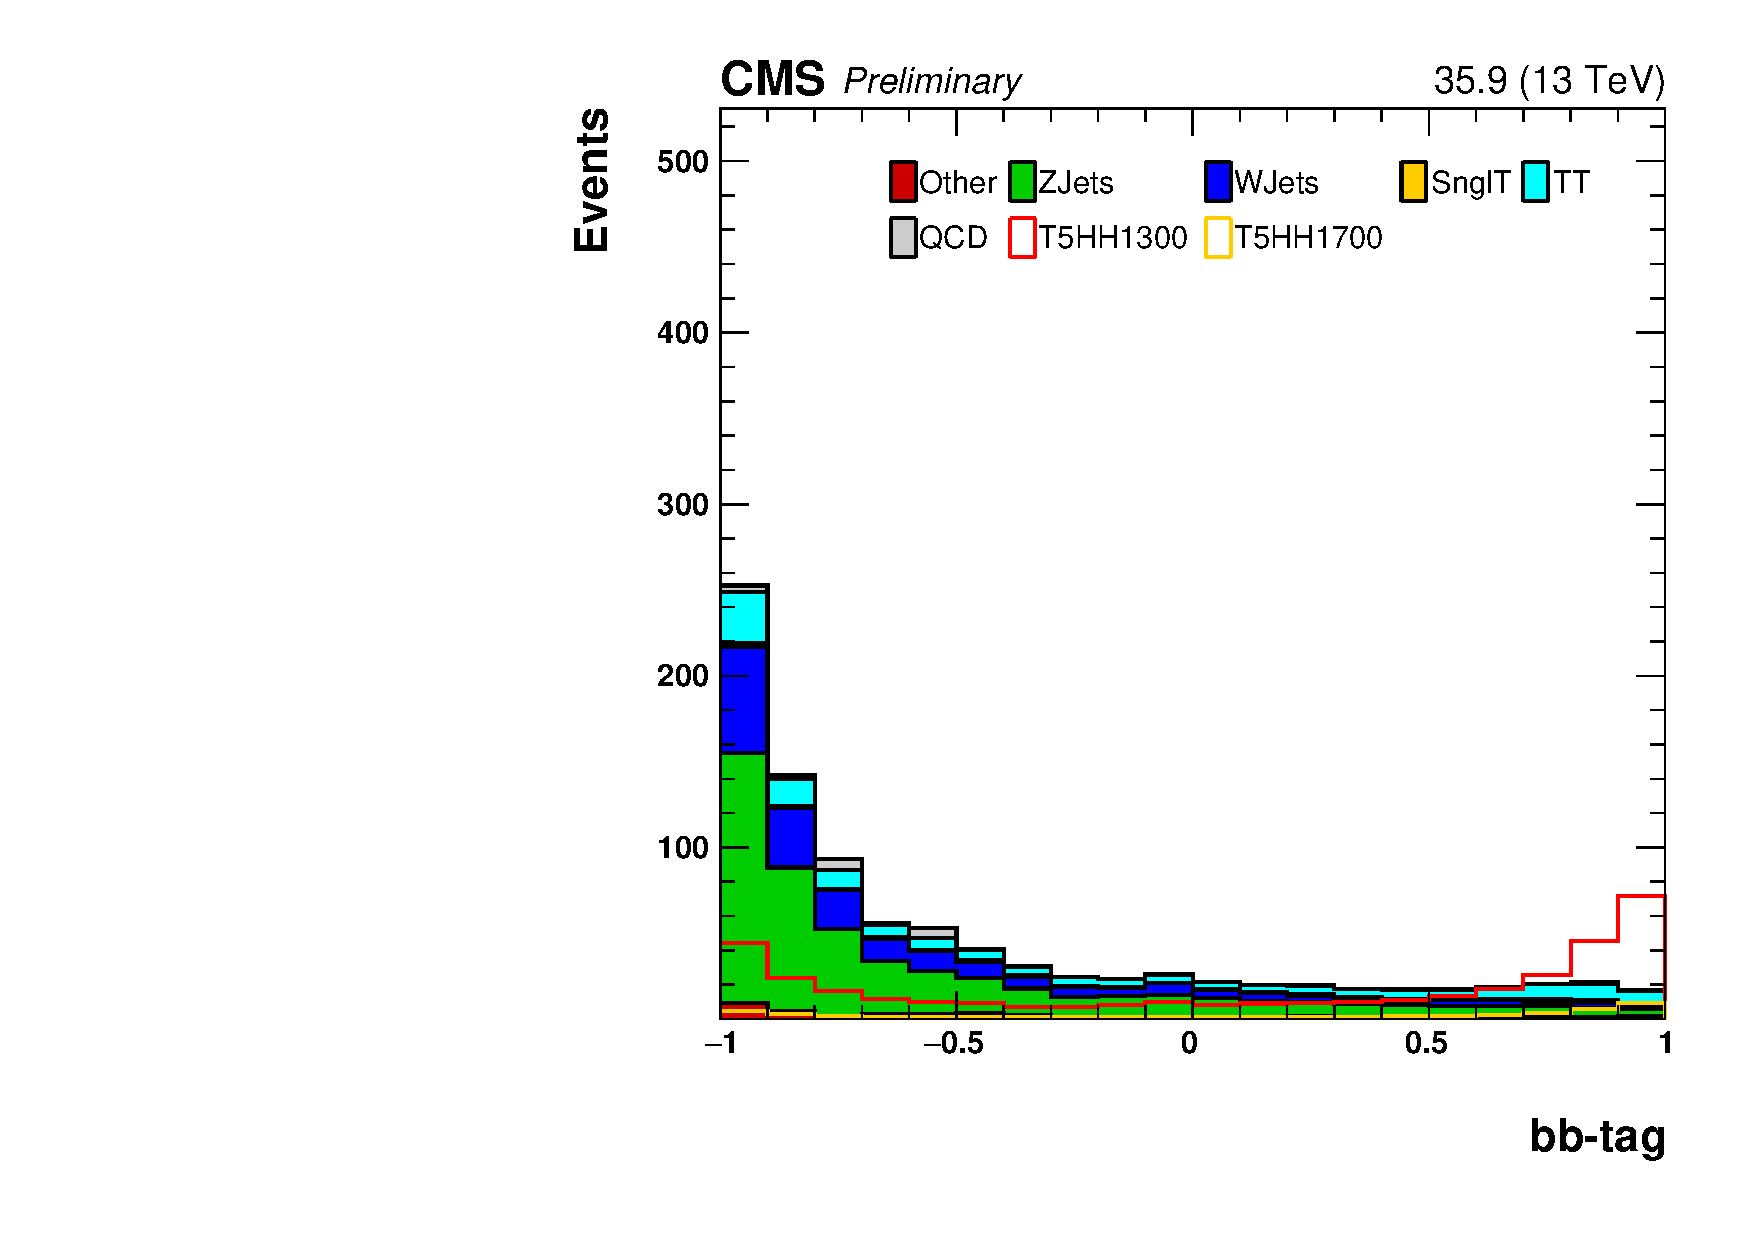
\includegraphics[width=0.425\linewidth]{figs/J2pt_BBtag_baseline.pdf}\\
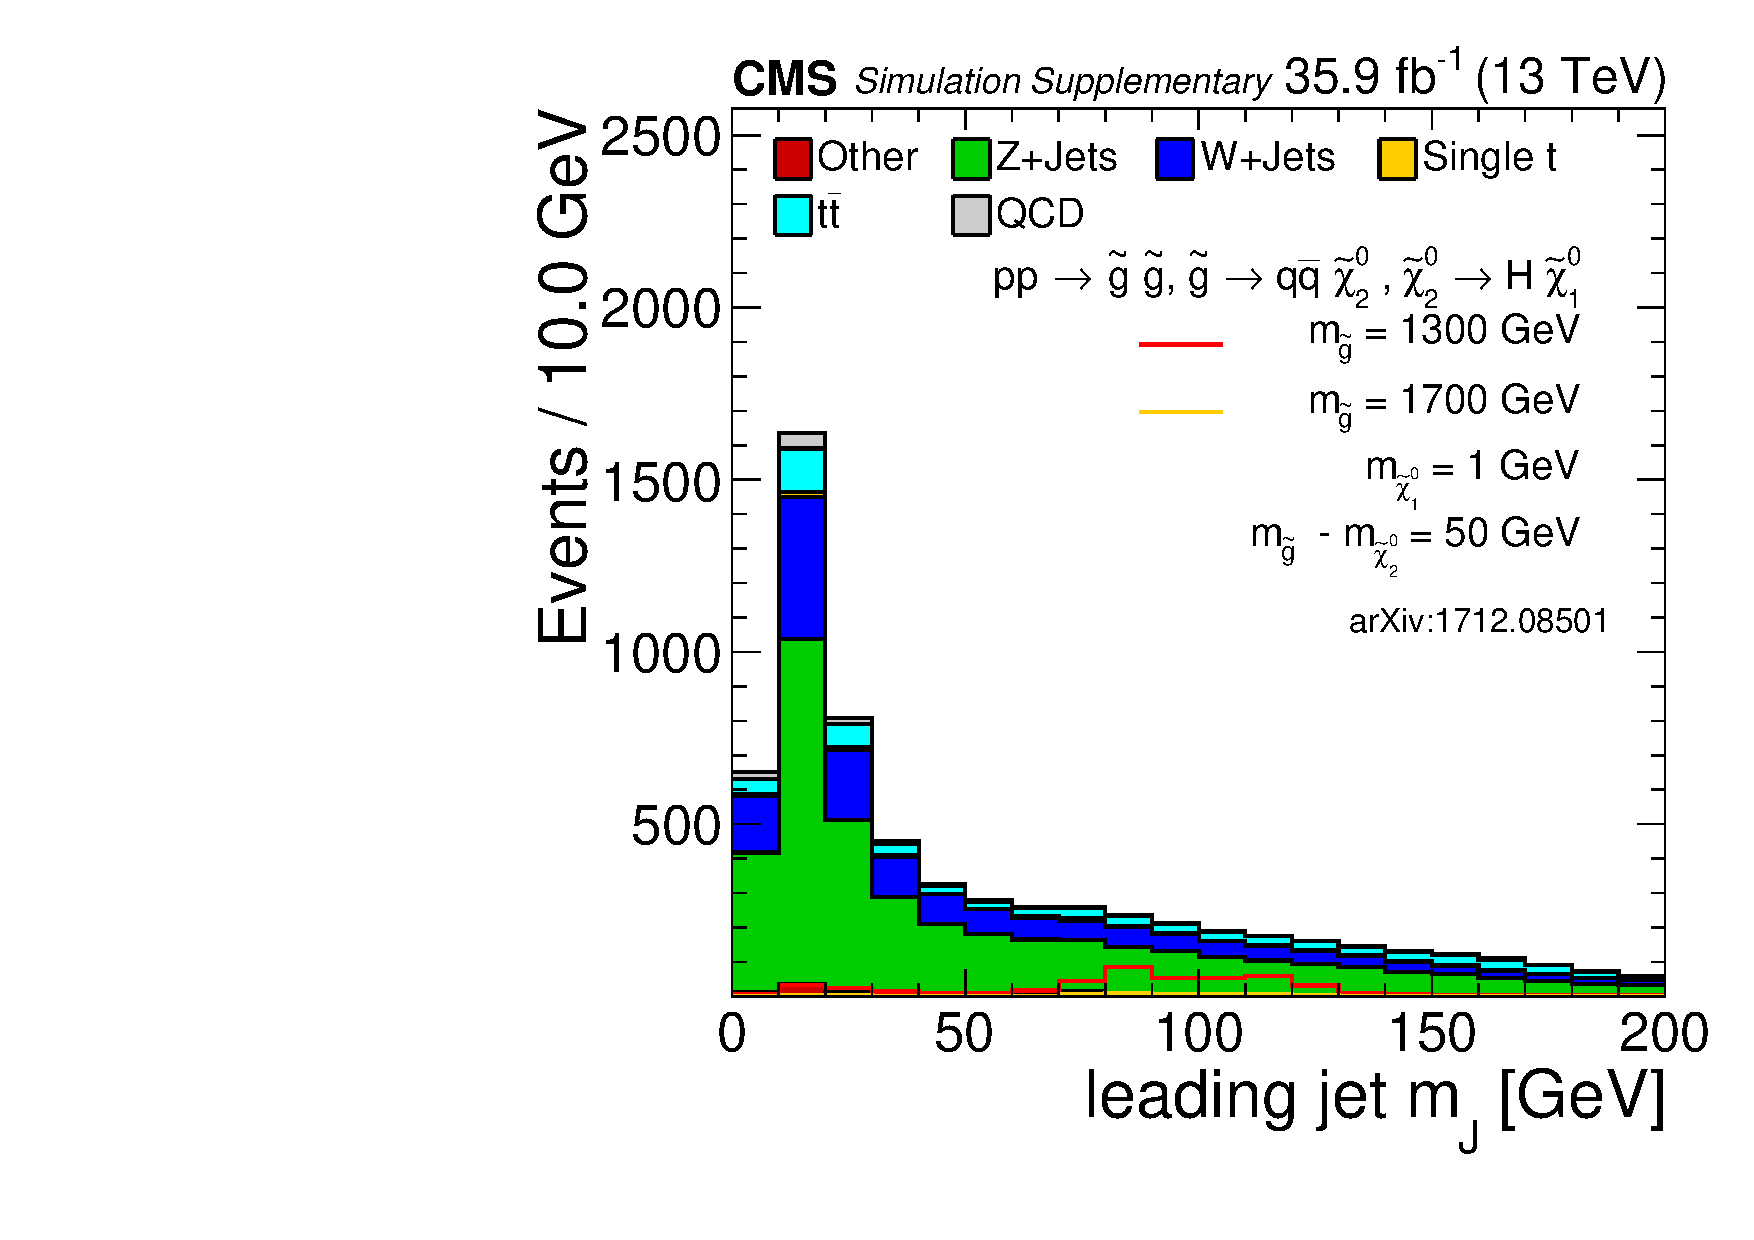
\includegraphics[width=0.425\linewidth]{figs/J1Mwide_JetPt.pdf}
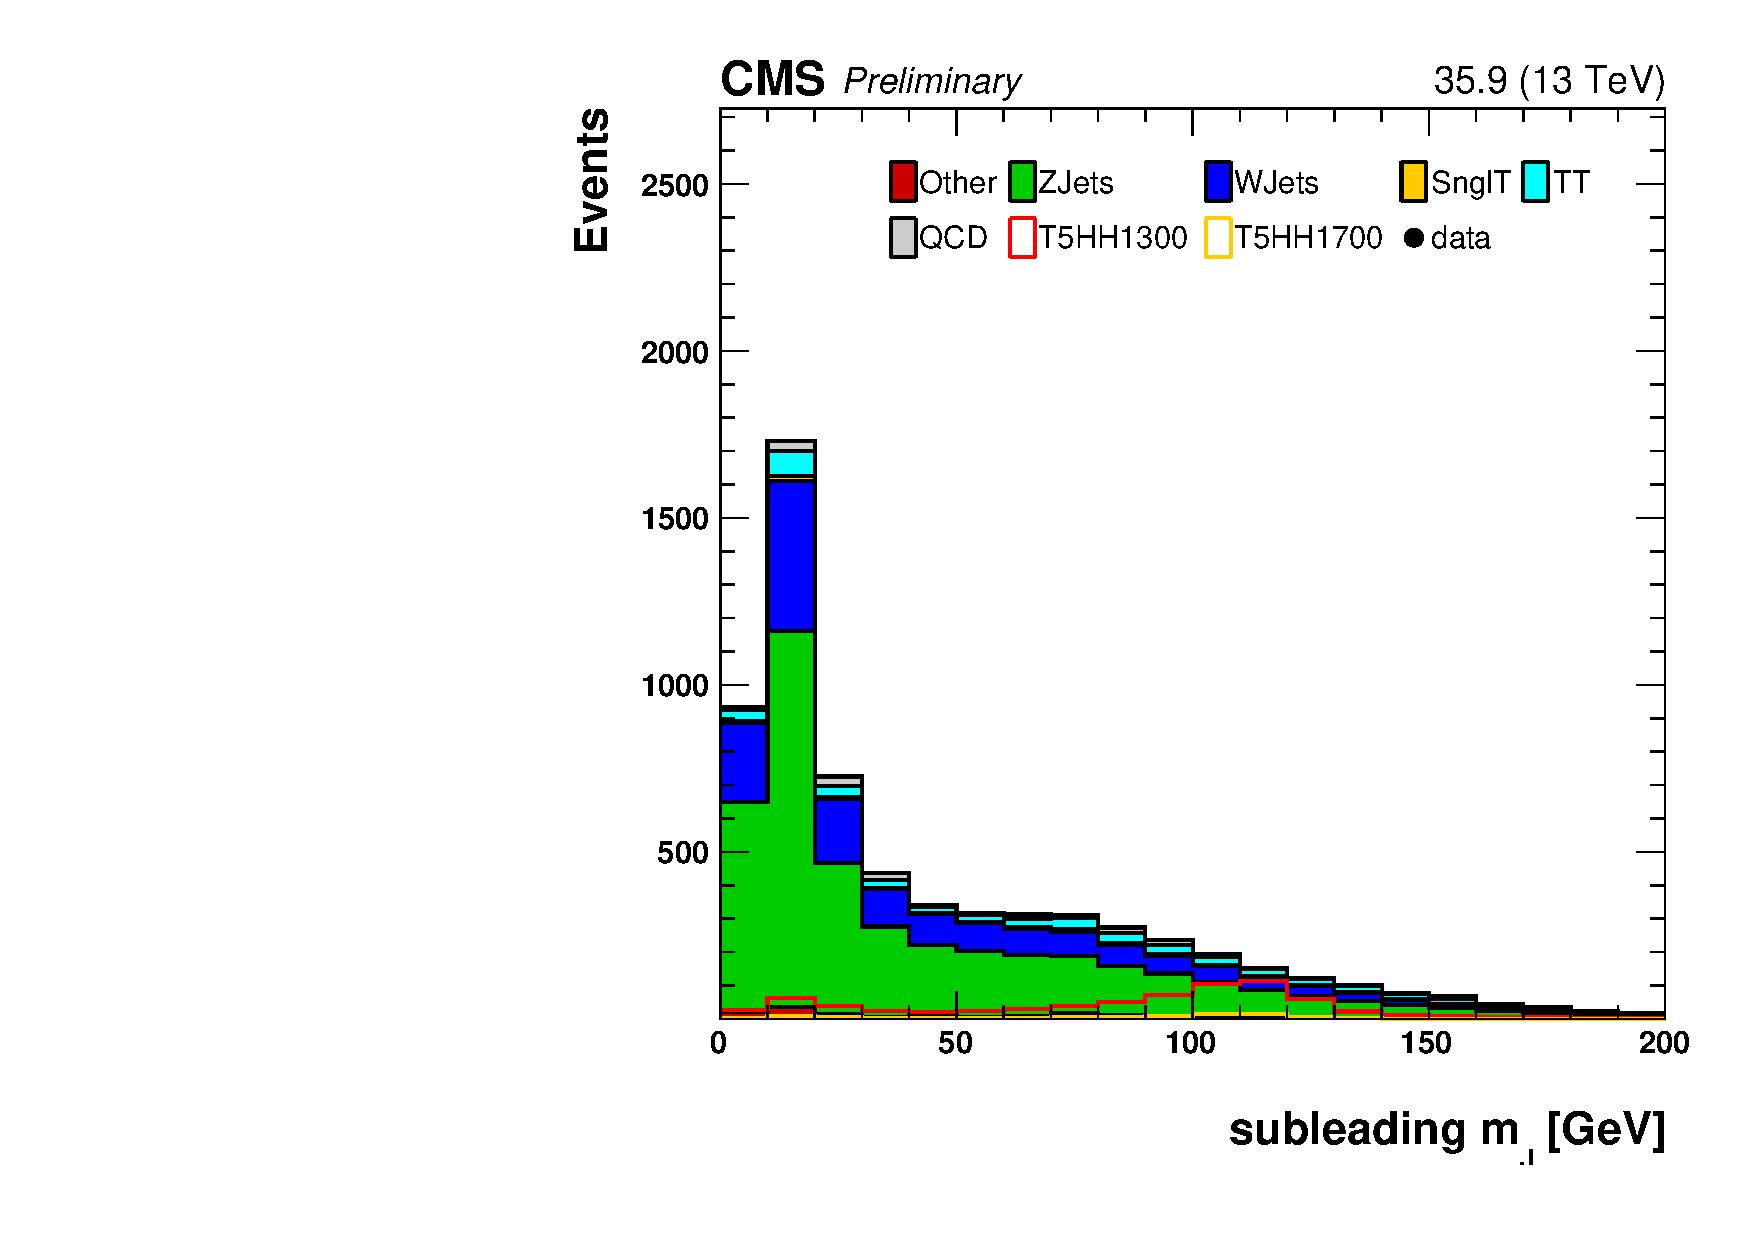
\includegraphics[width=0.425\linewidth]{figs/J2Mwide_JetPt.pdf}\\
\caption[Distributions of the bb-tagging discriminator and jet mass for AK8 jets.]
{Distributions of the bb-tagging discriminator (top row) and the jet mass (bottom row) for the leading (left column) and subleading (right column) AK8 jets. These are used in H/Z tagging of AK8 jets.}
\label{fig:ak8dists}
\end{figure}

\section{Dataset \& Trigger}

We use a total of 35.9 $\mathrm{fb}^{-1}$ of data collected by the CMS experiment in 2016. Events are selected in data using a trigger which requires greater than 100 GeV of \ptmiss calculated at high-level trigger (HLT); additionally the logical OR of two other triggers with thresholds of 110 and 120 GeV are applied. The trigger efficiency is derived in data using a single-electron reference trigger requiring a tight-ID electron of $p_{T}$$>$27 GeV. We further select events with at least three AK4 jets and exactly one reconstructed electron of $p_{T}$$>$25 GeV. The signal region trigger is found to be greater than 98\% for events with \ptmiss$>$250 GeV and HT$>$300 GeV \cite{CMS-SUS-16-033}.

\section{Event Simulation}

Event simulation of the proton-proton collisions proceeds in a step-wise manner.
To simulate the hard physics process MadGraph@NLO2.2.2 \cite{Alwall:2014hca} is used to calculate matrix-element amplitudes. The parton distribution functions (PDFs) used in these calculations are from NNPDF 3.0 \cite{Ball:2014uwa}.
Parton showering and other event dynamics are generated with Pythia \cite{pythiacite}.
The simulation of the interaction of the final state particles with the detector is performed with GEANT \cite{Agostinelli:2002hh}.
This ``raw'' simulation data is then at the same tier as data collected from the physical experiment and is merged into a single pipeline for event reconstruction.

\subsection{Standard Model Processes}
\label{sec:smp}

The SM samples which enter as the primary backgrounds are listed in Table~\ref{tab:mcsamples} (see Section~\ref{sec:smbkg} for a discussion of the SM background). All samples are generated with a pileup distribution with an average of 25 interactions per bunch crossing and a 25ns interval between bunches. For acceptable statistics over a wide range of parameter space, the MC samples are often binned in $\mathrm{HT}\equiv\sum_{AK4\,jets}p_{T}$. As our event selection requires at least two AK8 jets with $p_{T}$$>$300 GeV we roughly operate in regime of HT$>$600 GeV.

\begin{table}[hbp!]
\centering
\caption{SM MC samples used in the analysis.}
\label{tab:mcsamples}
\begin{tabular}{cclll}
\hline \hline
process & final state & HT (GeV) & $\sigma$ (pb) & $\int\mathcal{L}$ (fb$^{-1}$)\\
\hline
\ttbar & $t\rightarrow\ell\nu, \bar{t}\rightarrow2q$ & inclusive & 182.72 & 283.90\\
\ttbar & $\bar{t}\rightarrow\ell\nu, t\rightarrow2q$ & inclusive & 182.72 & 326.48\\
\ttbar & $2\ell$    & inclusive & 88.34 & 346.25\\
\ttbar & inclusive & [600, 800] & 2.734 & 5231.81\\
\ttbar & inclusive & [800, 1200] & 1.121 & 9416.61\\
\ttbar & inclusive & [1200, 2500]  & 0.198 & 14819.34\\
\ttbar & inclusive & [2500, $\infty$] & 0.002 & 221088.29\\
QCD & inclusive & [200, 300] & 1735000 & 0.03\\
QCD & inclusive & [300, 500] & 366800 & 0.16\\
QCD & inclusive & [500, 700] & 29370 & 1.95\\
QCD & inclusive & [700, 1000] & 6524 & 6.68\\
QCD & inclusive & [1000, 1500] & 1064 & 12.62\\
QCD & inclusive & [1500, 2000] & 121.5 & 32.63\\
QCD & inclusive & [2000, $\infty$] & 25.42 & 239.30\\
Z+jets & $\nu\bar{\nu}$ & [100, 200] & 344.8 & 54.13\\
Z+jets & $\nu\bar{\nu}$ & [200, 400] & 95.53 & 208.46\\
Z+jets & $\nu\bar{\nu}$ & [400, 600] & 13.20 & 77.30\\
Z+jets & $\nu\bar{\nu}$ & [600, 800] & 3.148 & 1795.26\\
Z+jets & $\nu\bar{\nu}$ & [800, 1200] & 1.451 & 1486.09\\
Z+jets & $\nu\bar{\nu}$ & [1200, 2500] & 0.355 & 1029.81\\
Z+jets & $\nu\bar{\nu}$ & [2500, $\infty$] & 0.0085 & 47498.87\\
W+jets & $\ell\nu$ & [100, 200] & 1627.45 & 18.16\\
W+jets & $\ell{\nu}$ & [200, 400] & 435.24 & 45.88\\
W+jets & $\ell{\nu}$ & [400, 600] & 59.18 & 123.64\\
W+jets & $\ell{\nu}$ & [600, 800] & 14.58 & 221.32\\
W+jets & $\ell{\nu}$ & [800, 1200] & 6.66 & 1123.13\\
W+jets & $\ell{\nu}$ & [1200, 2500] & 1.608 & 153.44\\
W+jets & $\ell{\nu}$ & [2500, $\infty$] & 0.039 & 6497.28\\
\hline \hline
\end{tabular}
\end{table}

\subsection{Signal Models}
\label{sec:signal-models}

For commissioning of the analysis technique (as well as the limit-setting procedure, see Section~\ref{sec:results}) Monte Carlo samples with our final-state signal topology were generated, as in Figure~\ref{fig:sms}. The signal sample follows the same processing chain as the SM samples. The mass splitting between the gluino $\tilde{g}$ and neutralino $\tilde{\chi}_{2}^{0}$ is fixed to 50 GeV, resulting in low $p_{T}$ SM quarks produced in the gluino $\tilde{g}$ decays. The mass of the neutralino $\chi^{0}_{1}$ (LSP) is fixed to 1 GeV. We have samples with a range of gluino $\tilde{g}$ masses from 750 to 2200 GeV. The $p_{T}$ distribution for the generated H bosons in these samples is seen in Figure~\ref{fig:GenHiggsBoost} for a number of gluino $\tilde{g}$ masses. Additionally the angular separation $\Delta R \equiv \sqrt{\Delta\phi^{2}+\Delta\eta^{2}}$ between the $b\bar{b}$ pair is shown. As the $p_{T}$ of a parent boson increases the $b\bar{b}$ pair from its decay tend to align, allowing complete reconstruction with a single AK8 jet.

\begin{figure}[hbp!]
\centering
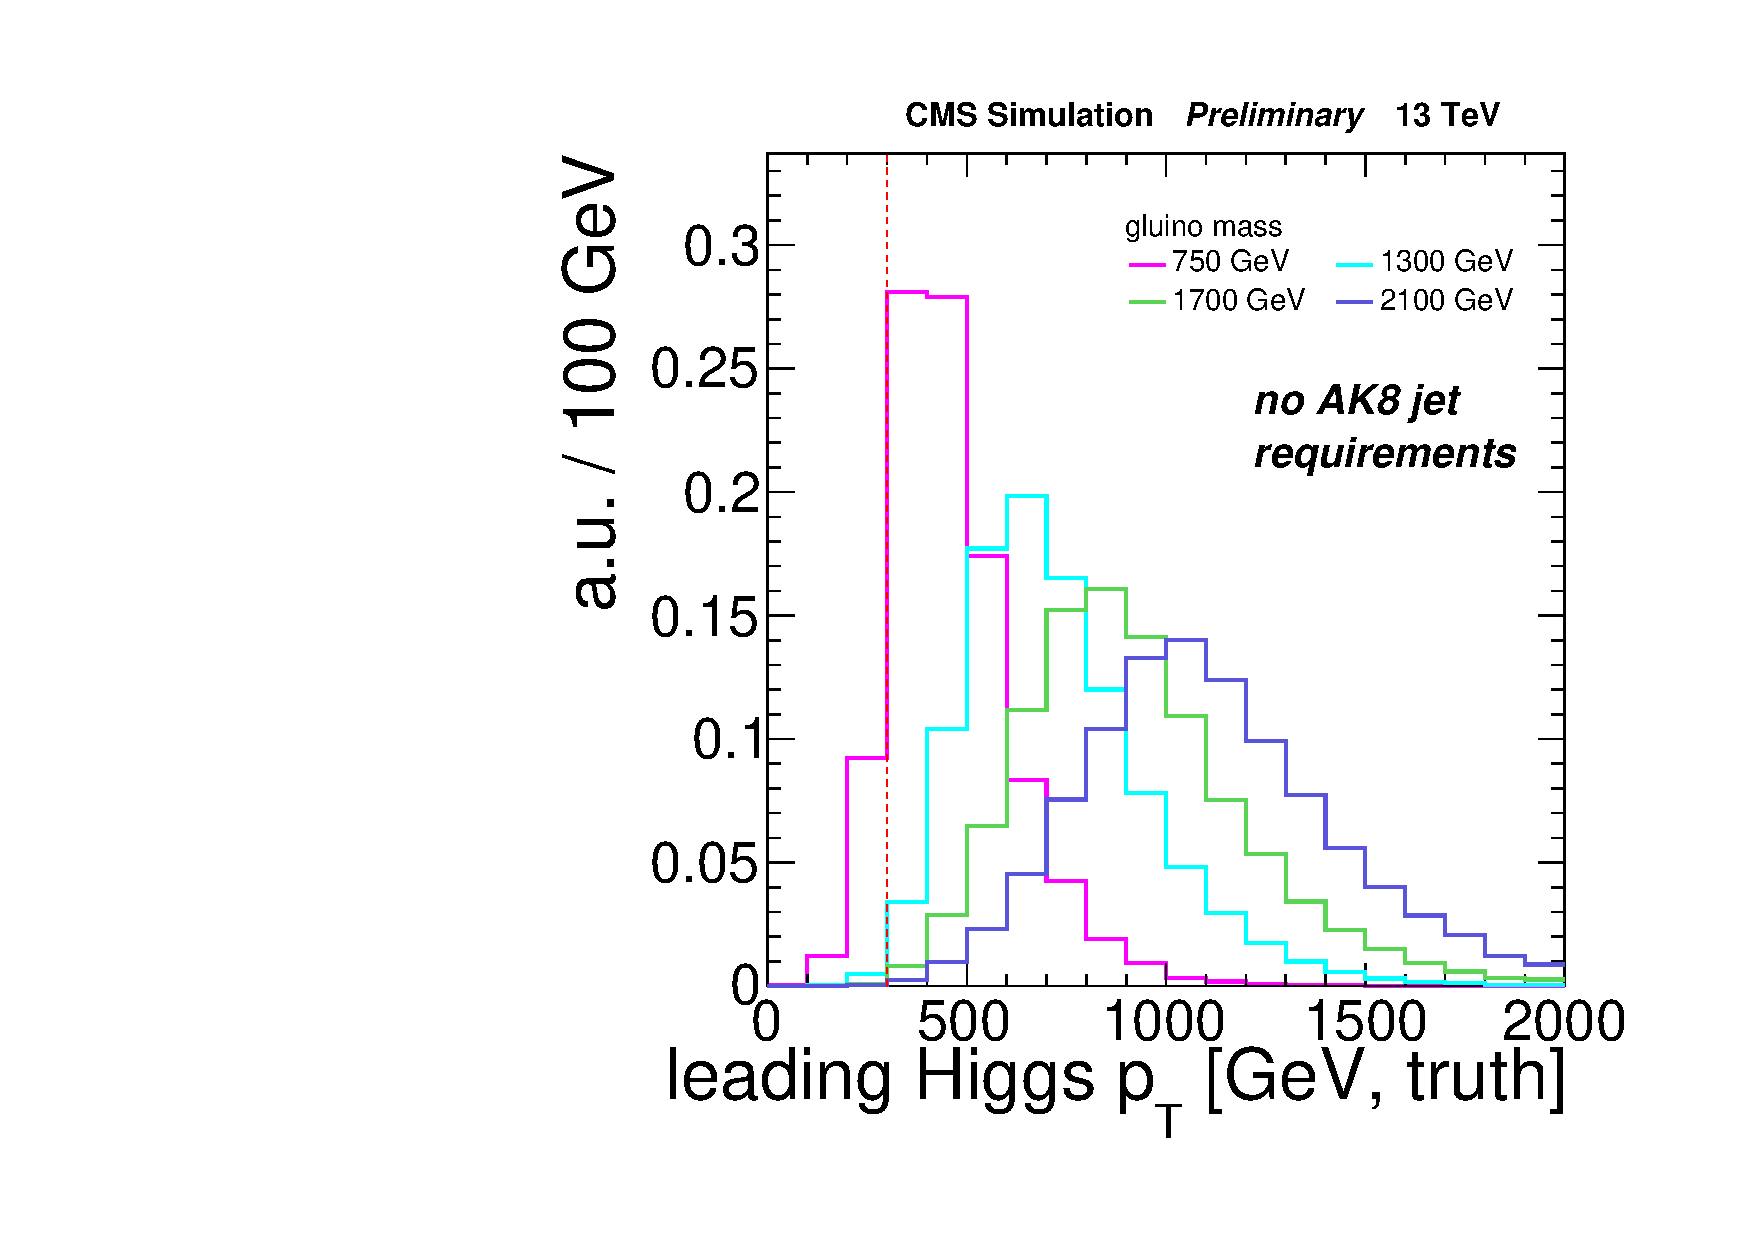
\includegraphics[width=0.45\linewidth]{figs/leadHiggsPt.pdf}
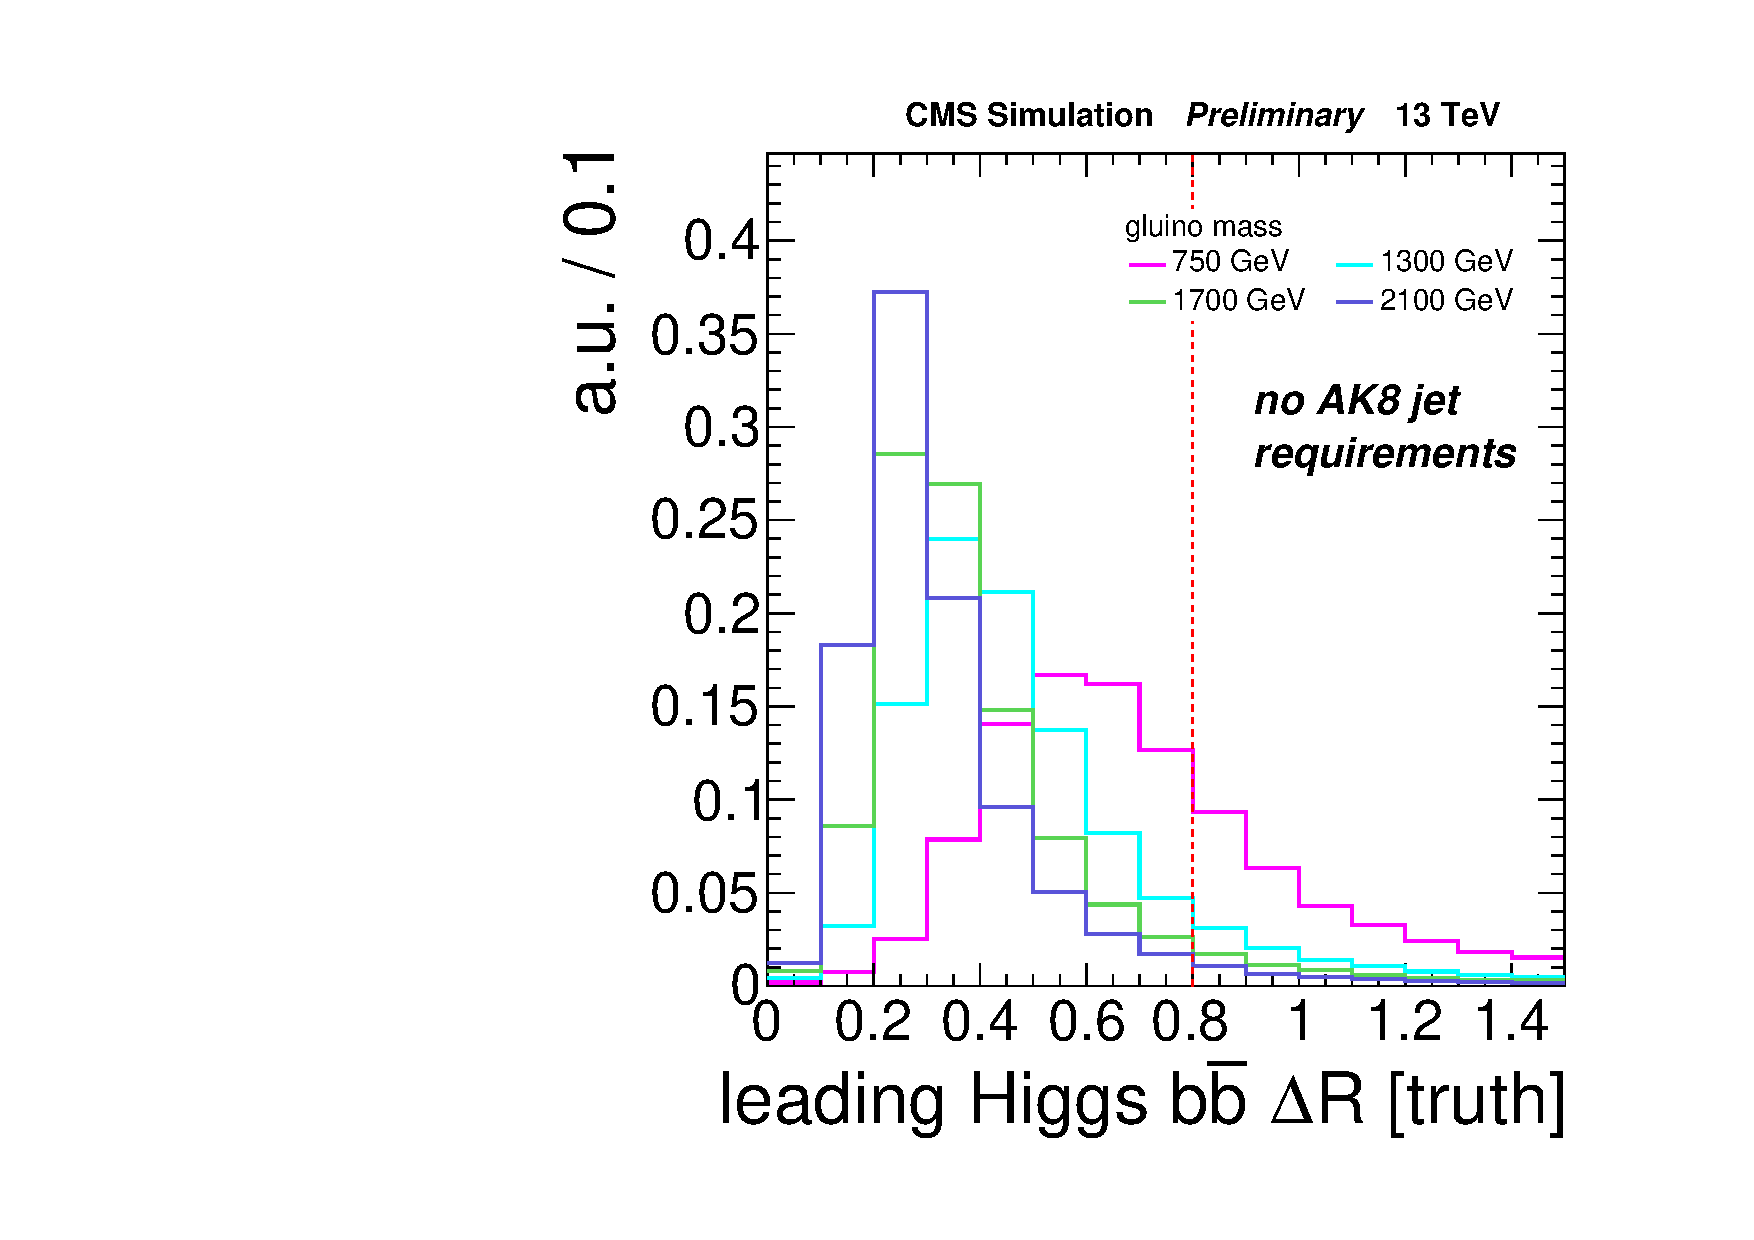
\includegraphics[width=0.45\linewidth]{figs/leadHiggsDr.pdf}\\
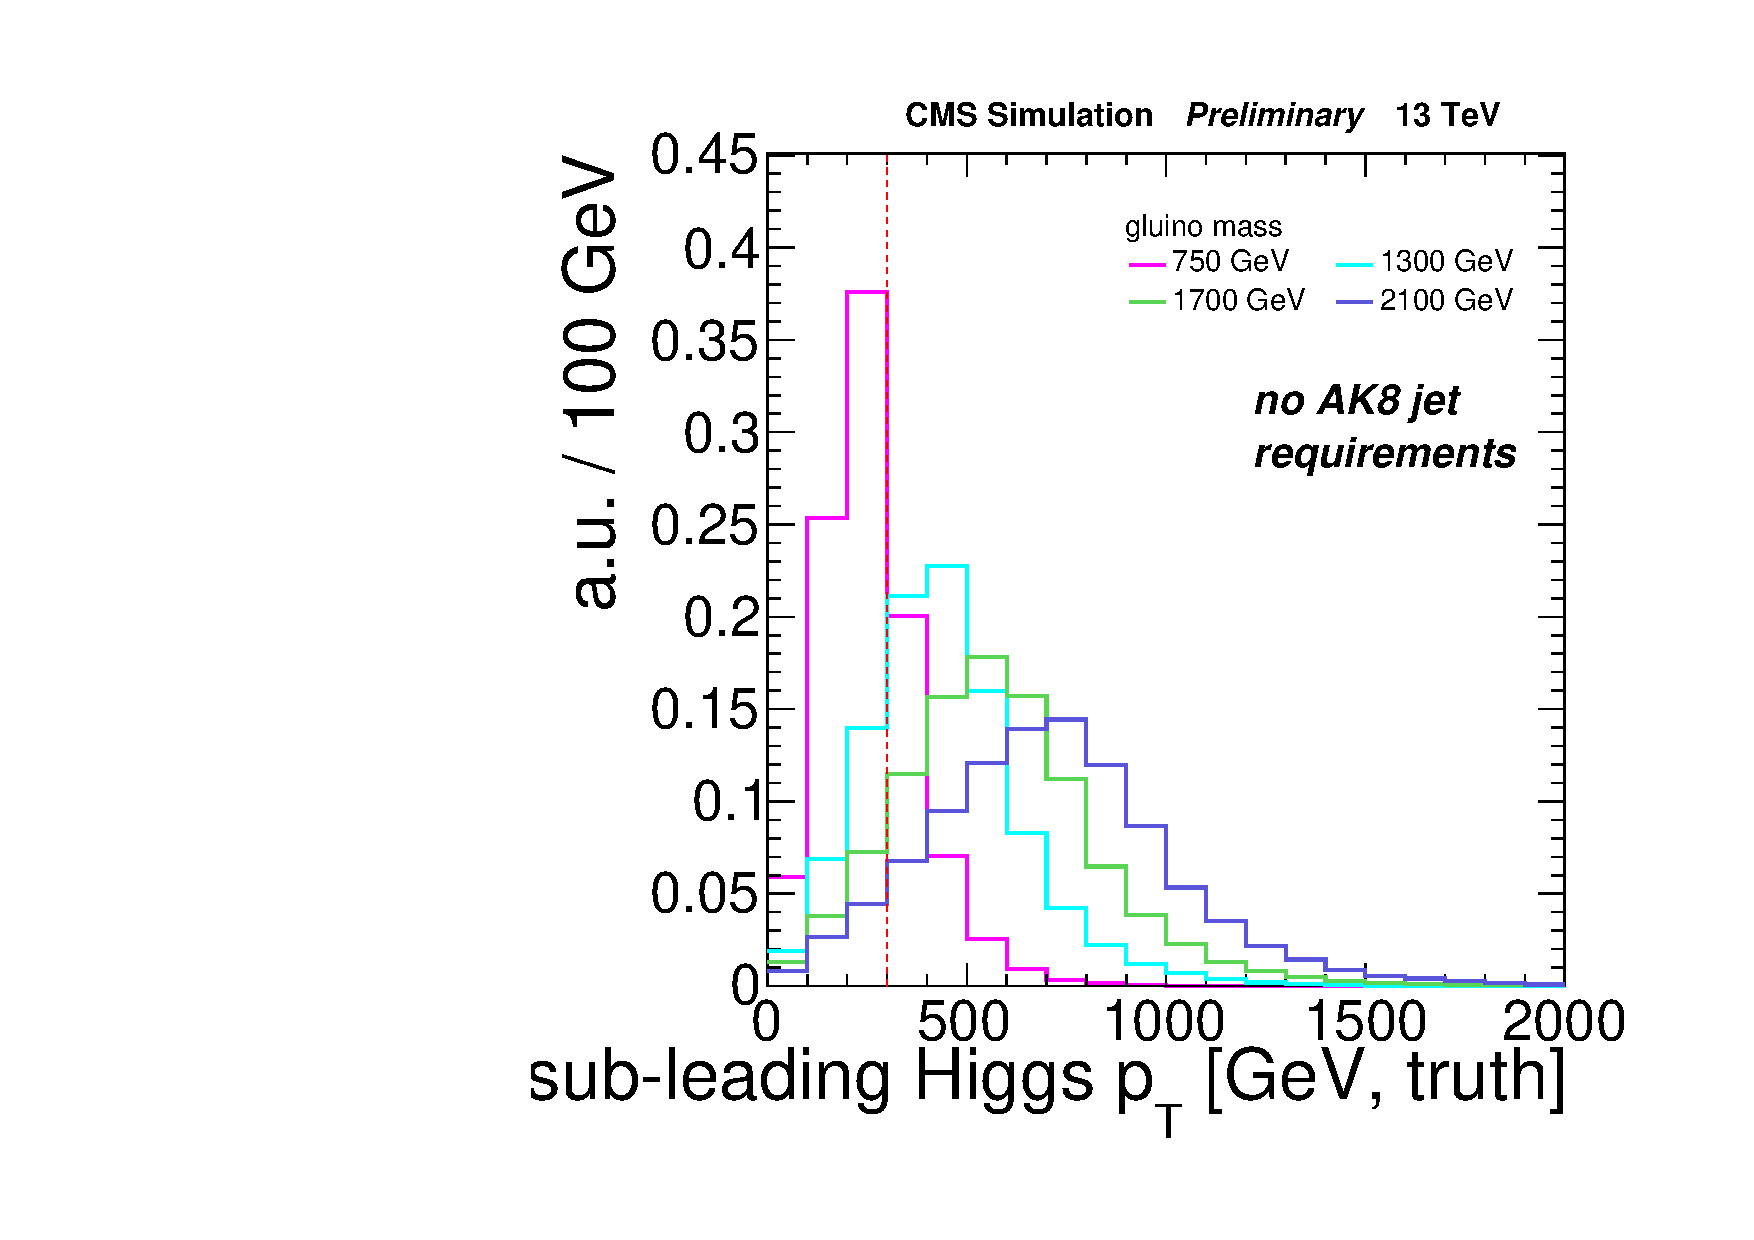
\includegraphics[width=0.45\linewidth]{figs/subleadHiggsPt.pdf}
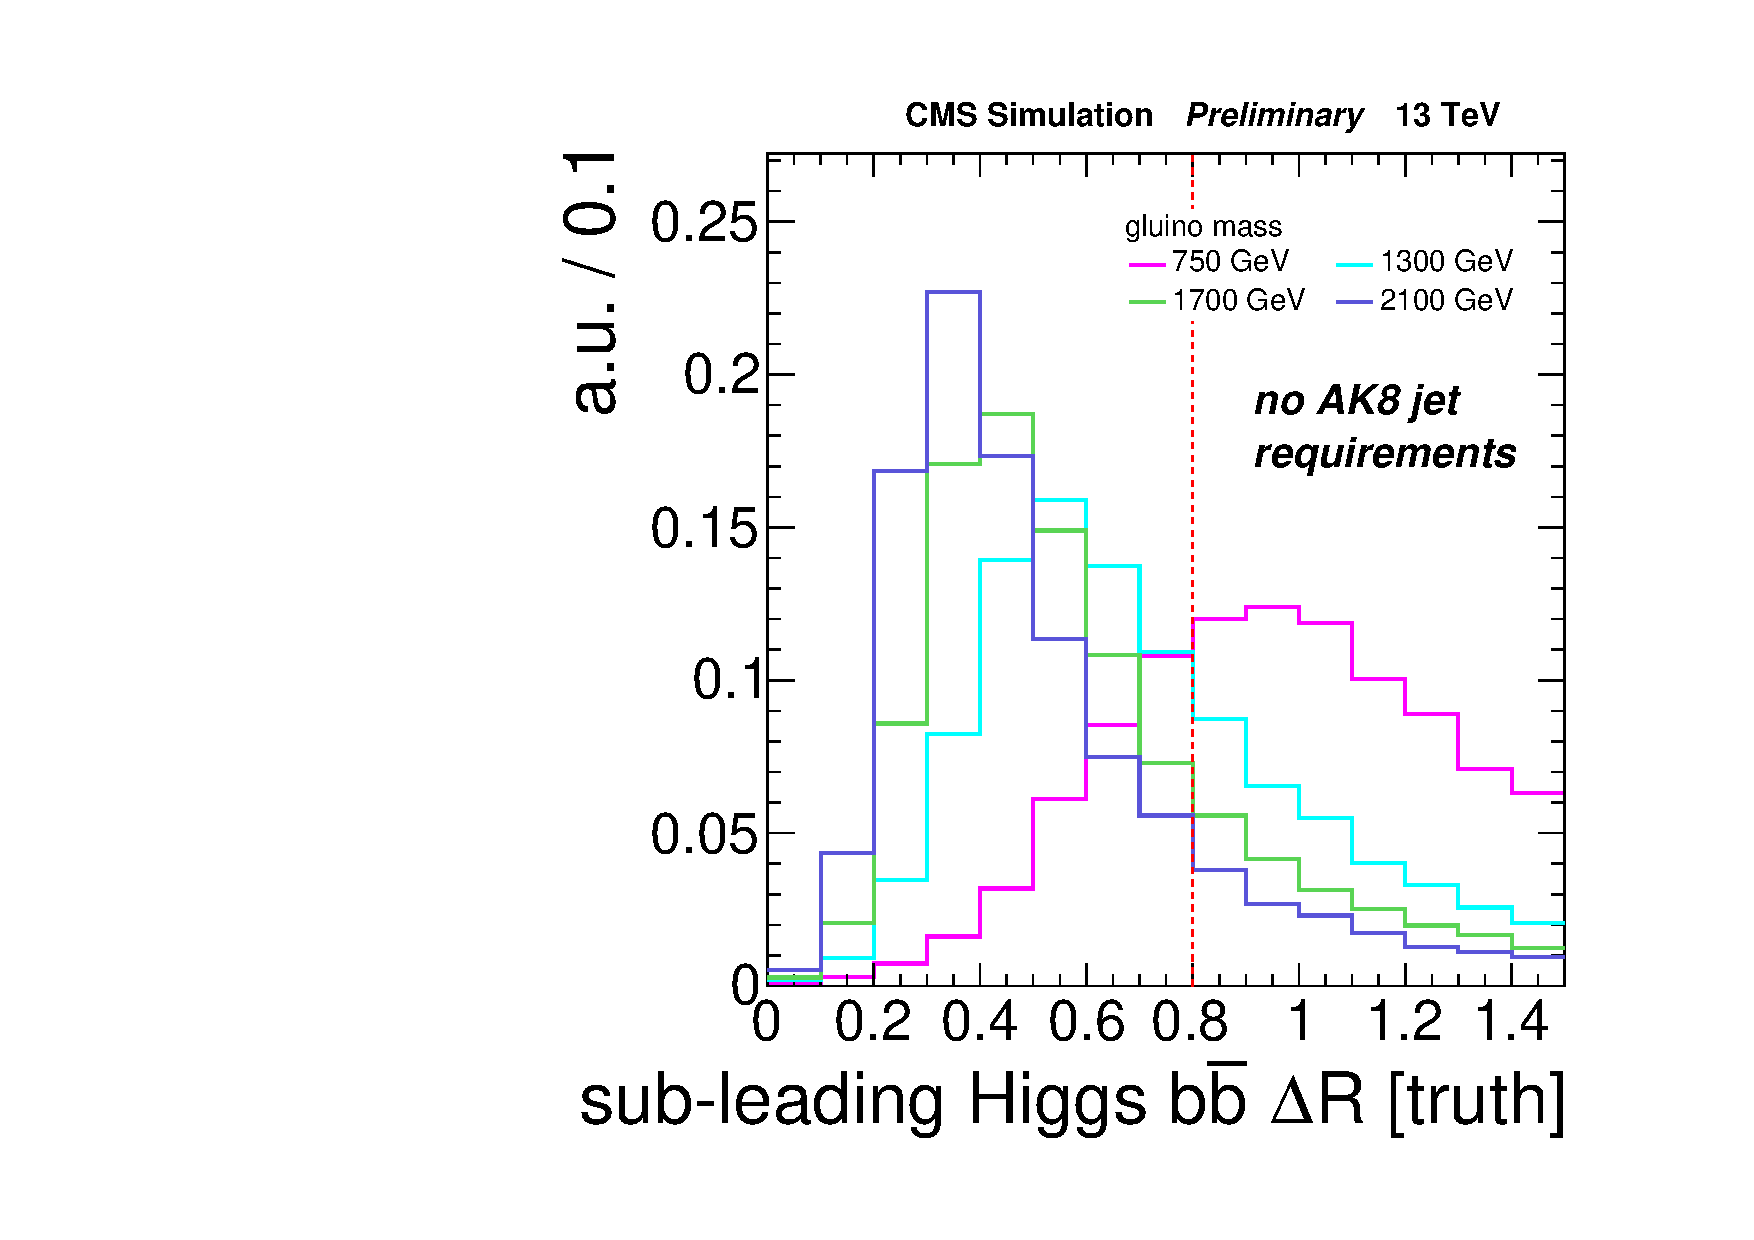
\includegraphics[width=0.45\linewidth]{figs/subleadHiggsDr.pdf}\\
\caption
[Generator level distributions for the H bosons in the T5HH model.]
{Generator level distributions for the leading (top row) and subleading (bottom row) H boson in the T5HH model. The plot on the left shows the $p_{T}$ of the H boson. The plot on right shows $\Delta R$ between the b-quark daughters - for large H $p_{T}$ the daughters become collimated.}
\label{fig:GenHiggsBoost}
\end{figure}

\section{Event Binning \& Background Estimation}

The background estimation procedure makes use of what is known as an ``ABCD'' prediction in which the analysis phase space is divided into signal and sideband regions; scaling relations are applied to sideband yields to make predictions for the SM background (inclusive in all processes) in the signal regions. The events are categorized according to whether the two leading AK8 jets are a) in the signal or sideband mass region and b) have or have not been $\mathrm{b}\bar{\mathrm{b}}$ tagged.  A diagram of this partitioning is seen in Figure~\ref{fig:abcd}. An additional dimension is added by binning in \ptmiss: [300, 500 GeV], [500, 700 GeV], [700, $\infty$ GeV]. This gives a total of 2x3=6 signal and 4x3=12 sideband bins. The two signal regions $\mathrm{A}_{1, 2}$ contain events with one (and only one) or two jets being consistent with H/Z boson decay, respectively.

\begin{figure}[hbp!]
\centering
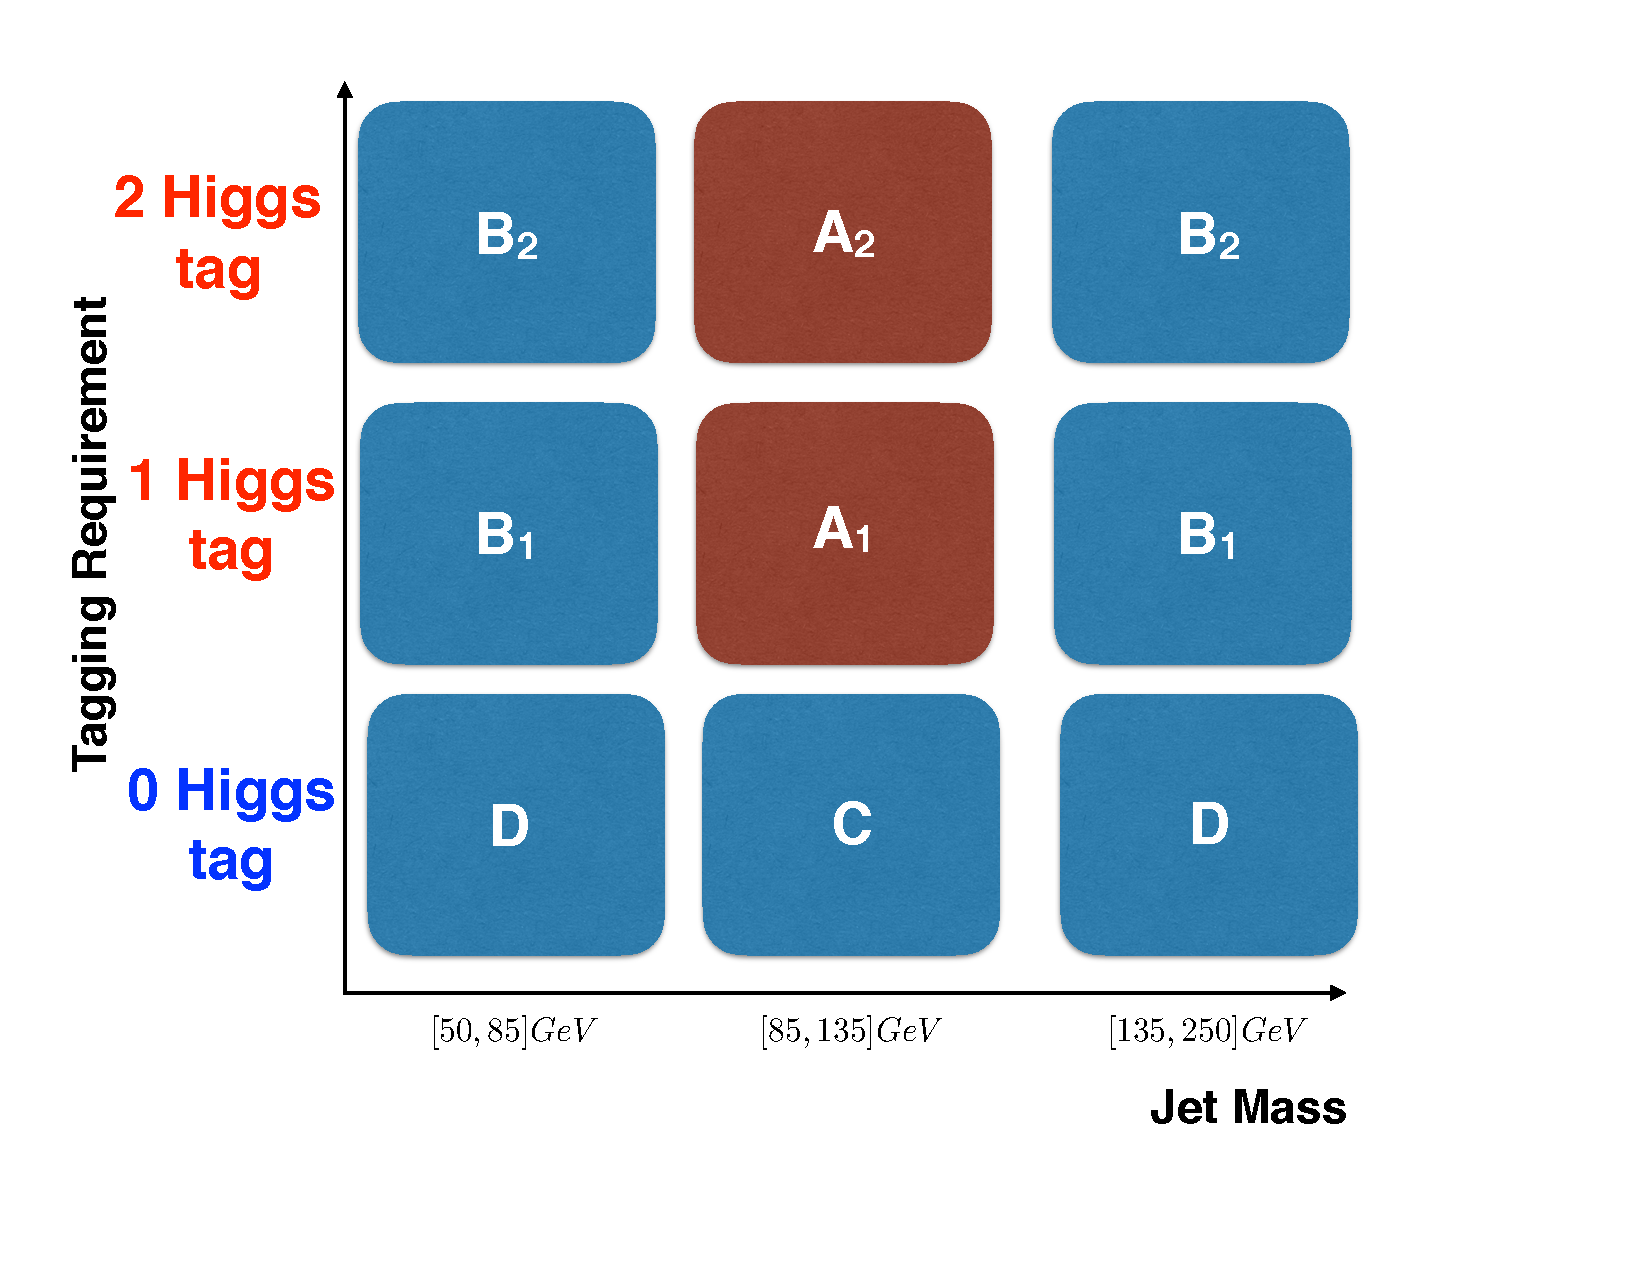
\includegraphics[width=0.6\textwidth]{figs/CMS-SUS-17-006_Figure-aux_002.pdf}
\caption[Partitioning of the signal and sideband regions for event binning.]{Partitioning of the signal and sideband regions for event binning. Additional binning in \ptmiss brings the total to 6x3=18.}
\label{fig:abcd}
\end{figure}

Assuming that there is no correlation between the jet mass and the $b\bar{b}$ tagging one would expect that

\begin{equation}
\frac{\mathrm{A}_{1, 2}}{\mathrm{B}_{1, 2}} = \frac{\mathrm{C}}{\mathrm{D}}
\end{equation}

Rearranging this gives a prediction for the events in the signal regions

\begin{equation}
\mathrm{A}_{1, 2}^{\mathrm{predicted}} = (\mathrm{B}_{1, 2} \cdot \frac{\mathrm{C}}{\mathrm{D}})^{\mathrm{observed}}
\end{equation}

The expected \ptmiss distribution from simulation is seen in the stacked histograms of Figure~\ref{fig:mcclosure}. The prediction using the ABCD method is seen in the red hash. The performance of the method within simulation can be determined by dividing the true content in the signal region with the prediction. This ratio, denoted $\kappa$, is seen in the bottom panel of Figure~\ref{fig:mcclosure}. $\kappa=1$ represents perfect modeling. As will be discussed in Section~\ref{sec:kappa}, $\kappa$ is used as a correction in the background estimation procedure.

\begin{figure}[hbp!]
\centering
\begin{subfigure}[b]{0.49\textwidth}
\centering
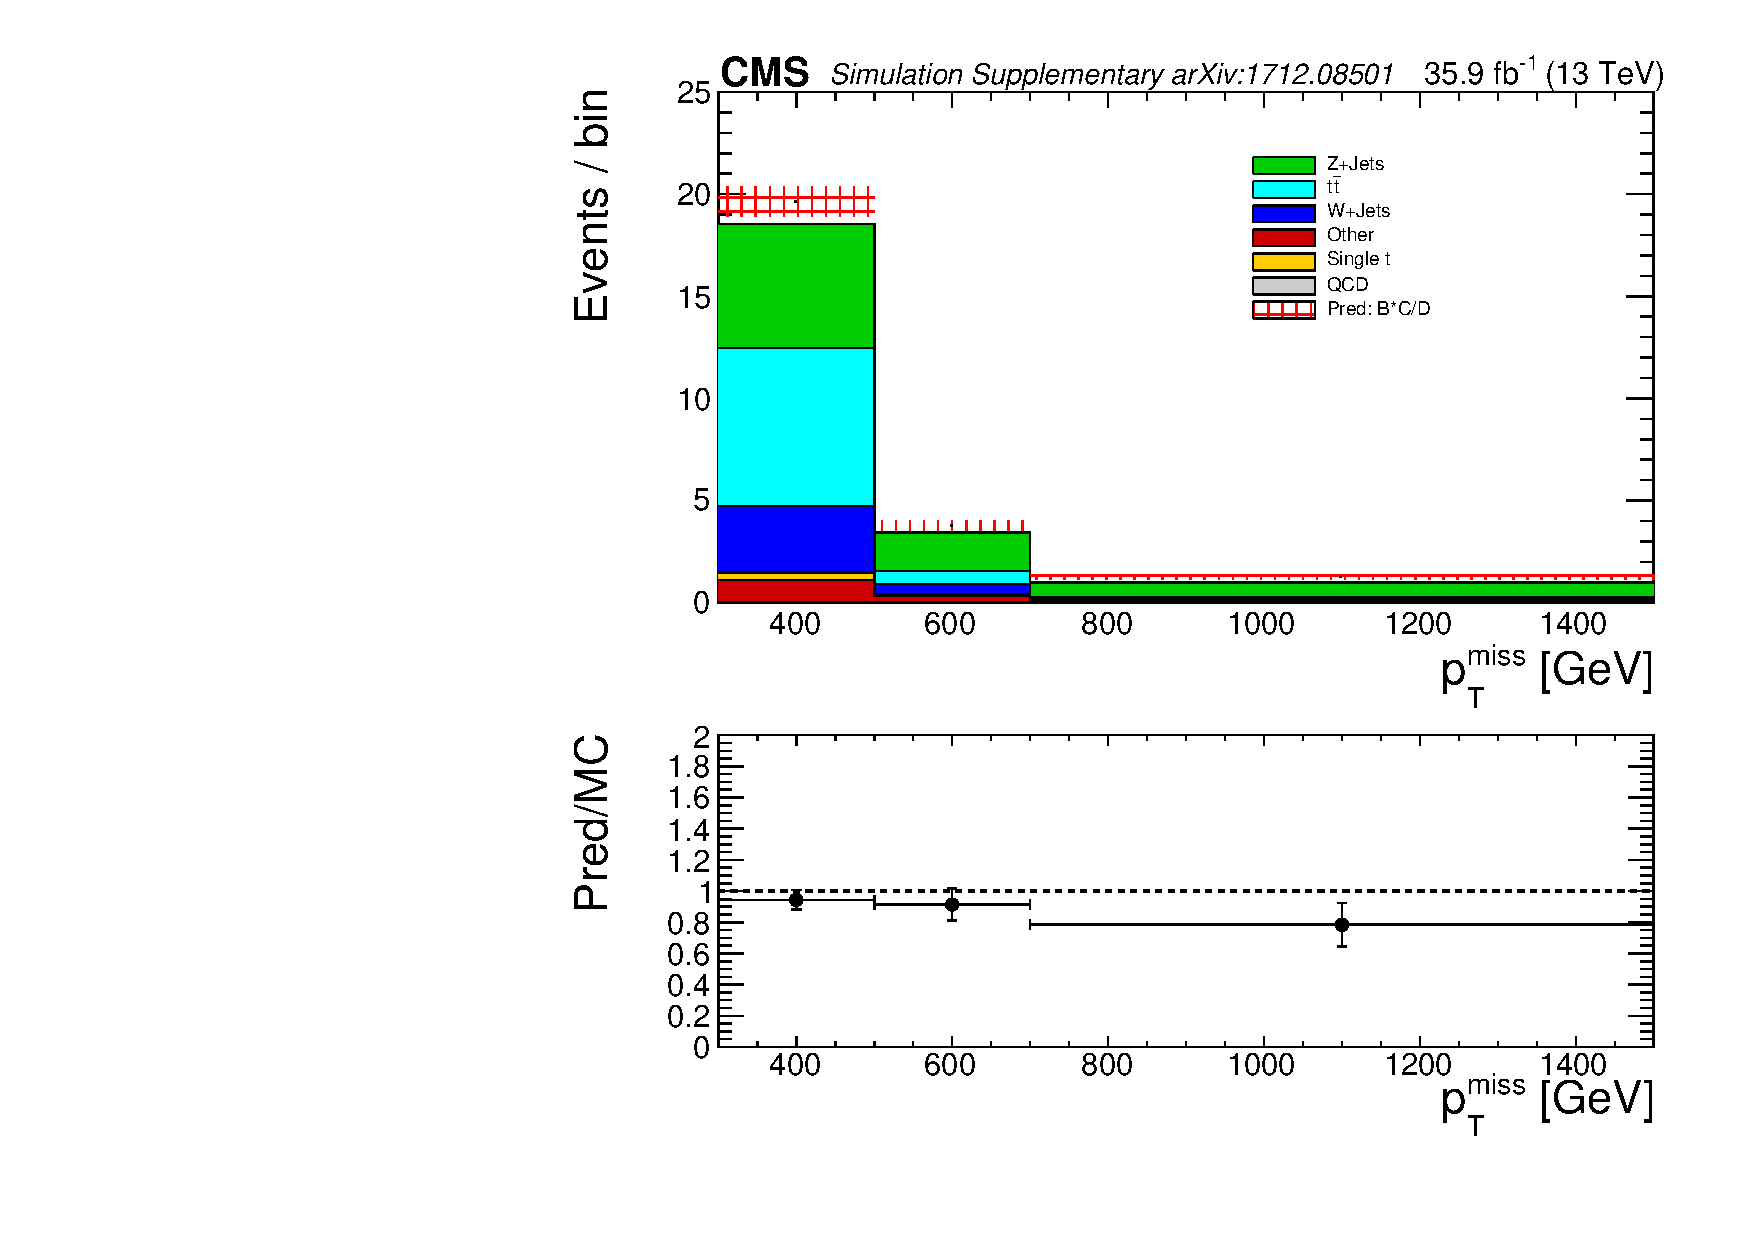
\includegraphics[trim={5px 5px 5px 5px},clip,width=0.95\textwidth]{figs/MCclosure_singleHiggsRegionTotal.pdf}
\caption{The single Higgs tag region (A$_{1}$).}
\end{subfigure}
\begin{subfigure}[b]{0.49\textwidth}
\centering
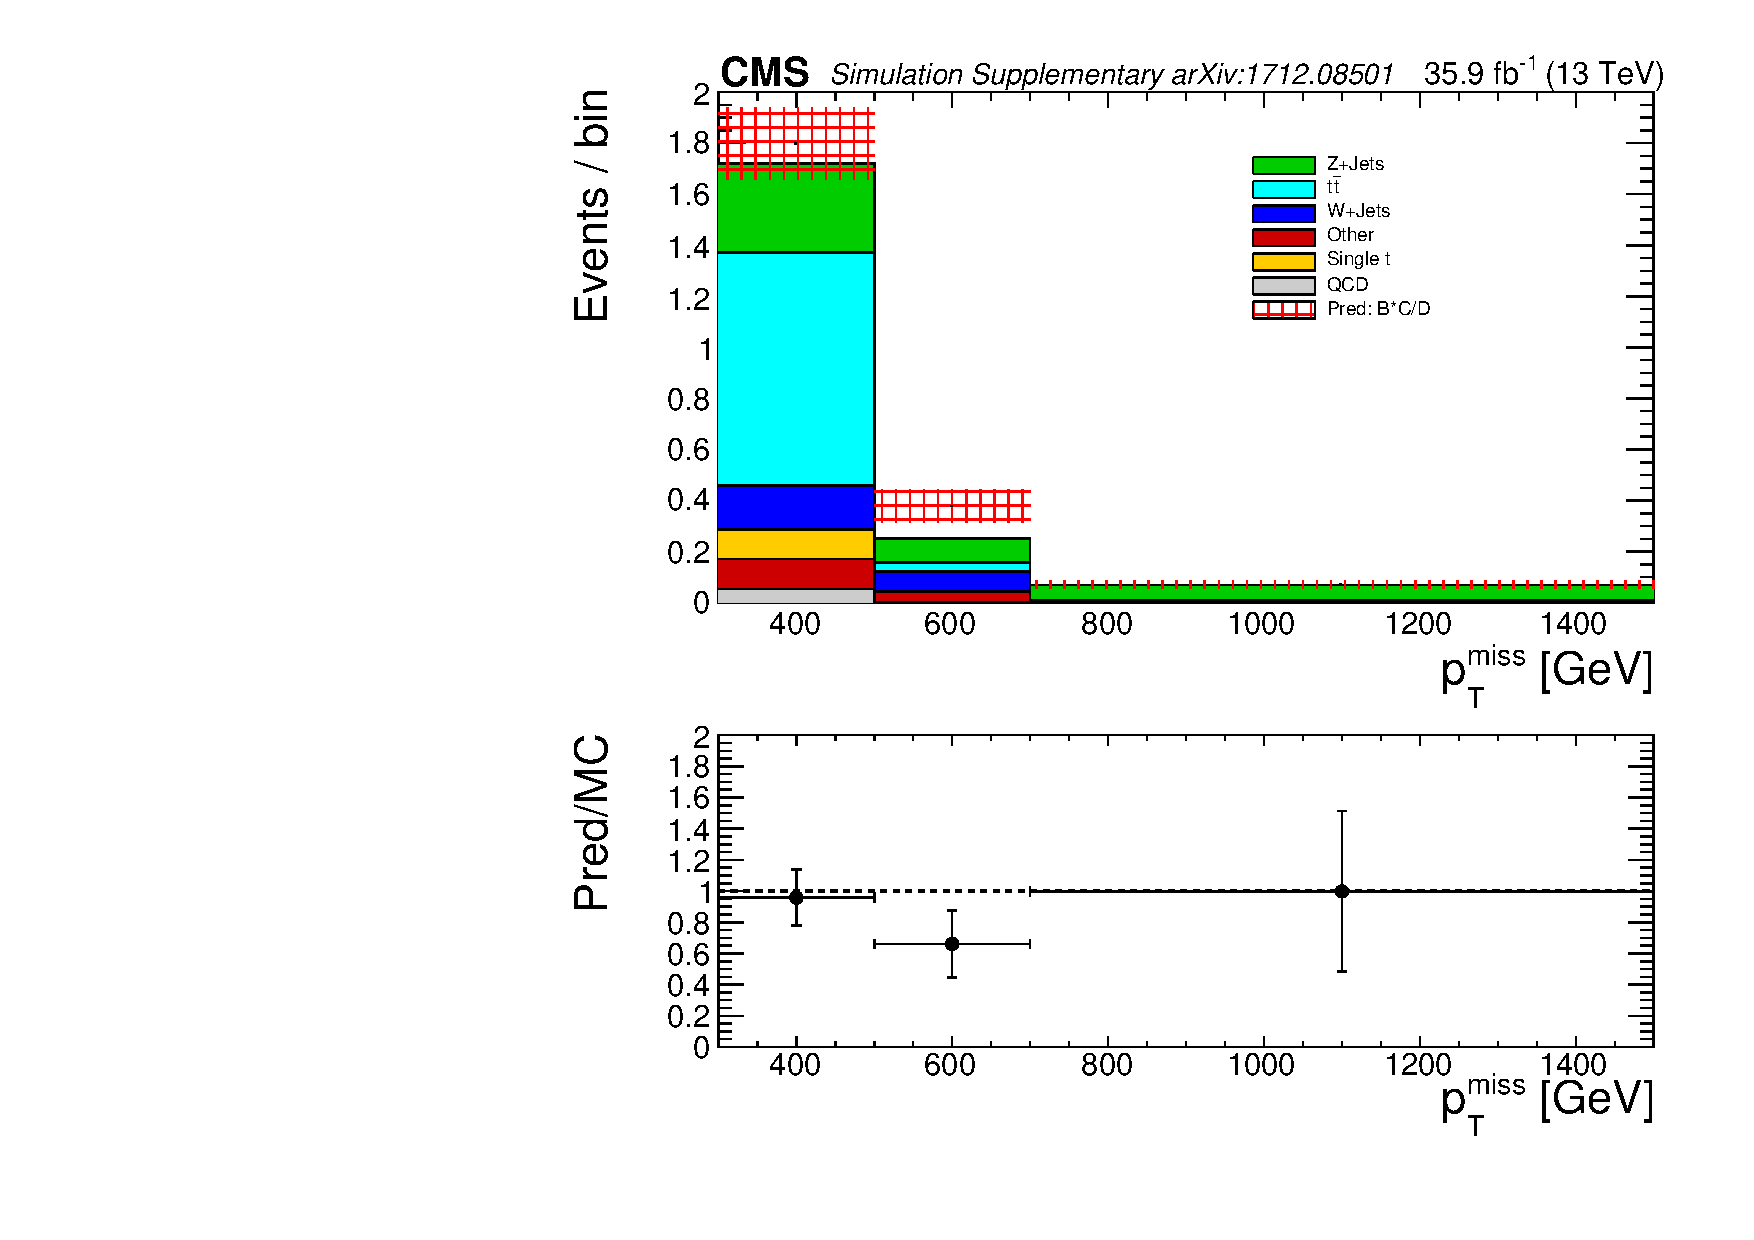
\includegraphics[trim={5px 5px 5px 5px},clip,width=0.95\textwidth]{figs/MCclosure_doubleHiggsRegionTotal.pdf} 
\caption{The double Higgs tag region (A$_{2}$).}
\end{subfigure}
\caption{\ptmiss distributions and predictions in the signal regions using simulation only.}
\label{fig:mcclosure}
\end{figure}

\subsection{Control Regions within Data}
\label{sec:smbkg}

We treat the SM backgrounds in the analysis as consisting of three main components (hinted at the list of MC samples seen in Table~\ref{tab:mcsamples}):

\begin{itemize}
\item $Z\rightarrow\nu\bar{\nu}$ in which the invisible Z gives true \ptmiss (`Z-invisible').
\item Semi-leptonic W or t production in which the lepton is not identified, the associated neutrino from the leptonic decay creates true \ptmiss (`lost-lepton').
\item Jet production via QCD in which the $p_{T}$ of a jet is substantially under-measured, this creates a fake source of \ptmiss.
\end{itemize}

Three control regions are defined to serve as a proxy for each source. They are defined with the same event selection as the signal and control regions, with the exception of the inversion of a single cut.

\begin{itemize}
\item A control region with a single-photon, after artificially removing the photon from event reconstruction, closely mimics the Z-invisible background. For high-$p_{T}$, both photons and Z bosons become massless, neutral, gauge bosons whose kinematics are expected to be similar.
\item A control region with a single-lepton, mimics the lost-lepton background.
\item A control region defined by the logical inversion of the low-$\Delta\phi$ cuts, most closely mimics the QCD background. This enriches our events with those likely in which \ptmiss is aligned with an under-measured AK4 jet.
\end{itemize}

As they are orthogonal to the analysis region, we are able to test the validuty of the background estimation technique independently within each of the three control regions. By comparing the prediction of the SM yields (using the ABCD method) with those observed, the validity of the technique can be verified for that particular background category. The comparisons for the single-photon, single-lepton and low-$\Delta\phi$ control regions can be seen in Figure~\ref{fig:closure}. $\kappa$ in the bottom panel is defined as the ratio of the true event yield to the prediction. $\kappa=1$ represents the case in which the prediction perfectly matches the observation. These comparisons are used for commissioning of the background estimation technique only.

\begin{figure}[hbp!]
\centering
\begin{subfigure}[b]{0.425\textwidth}
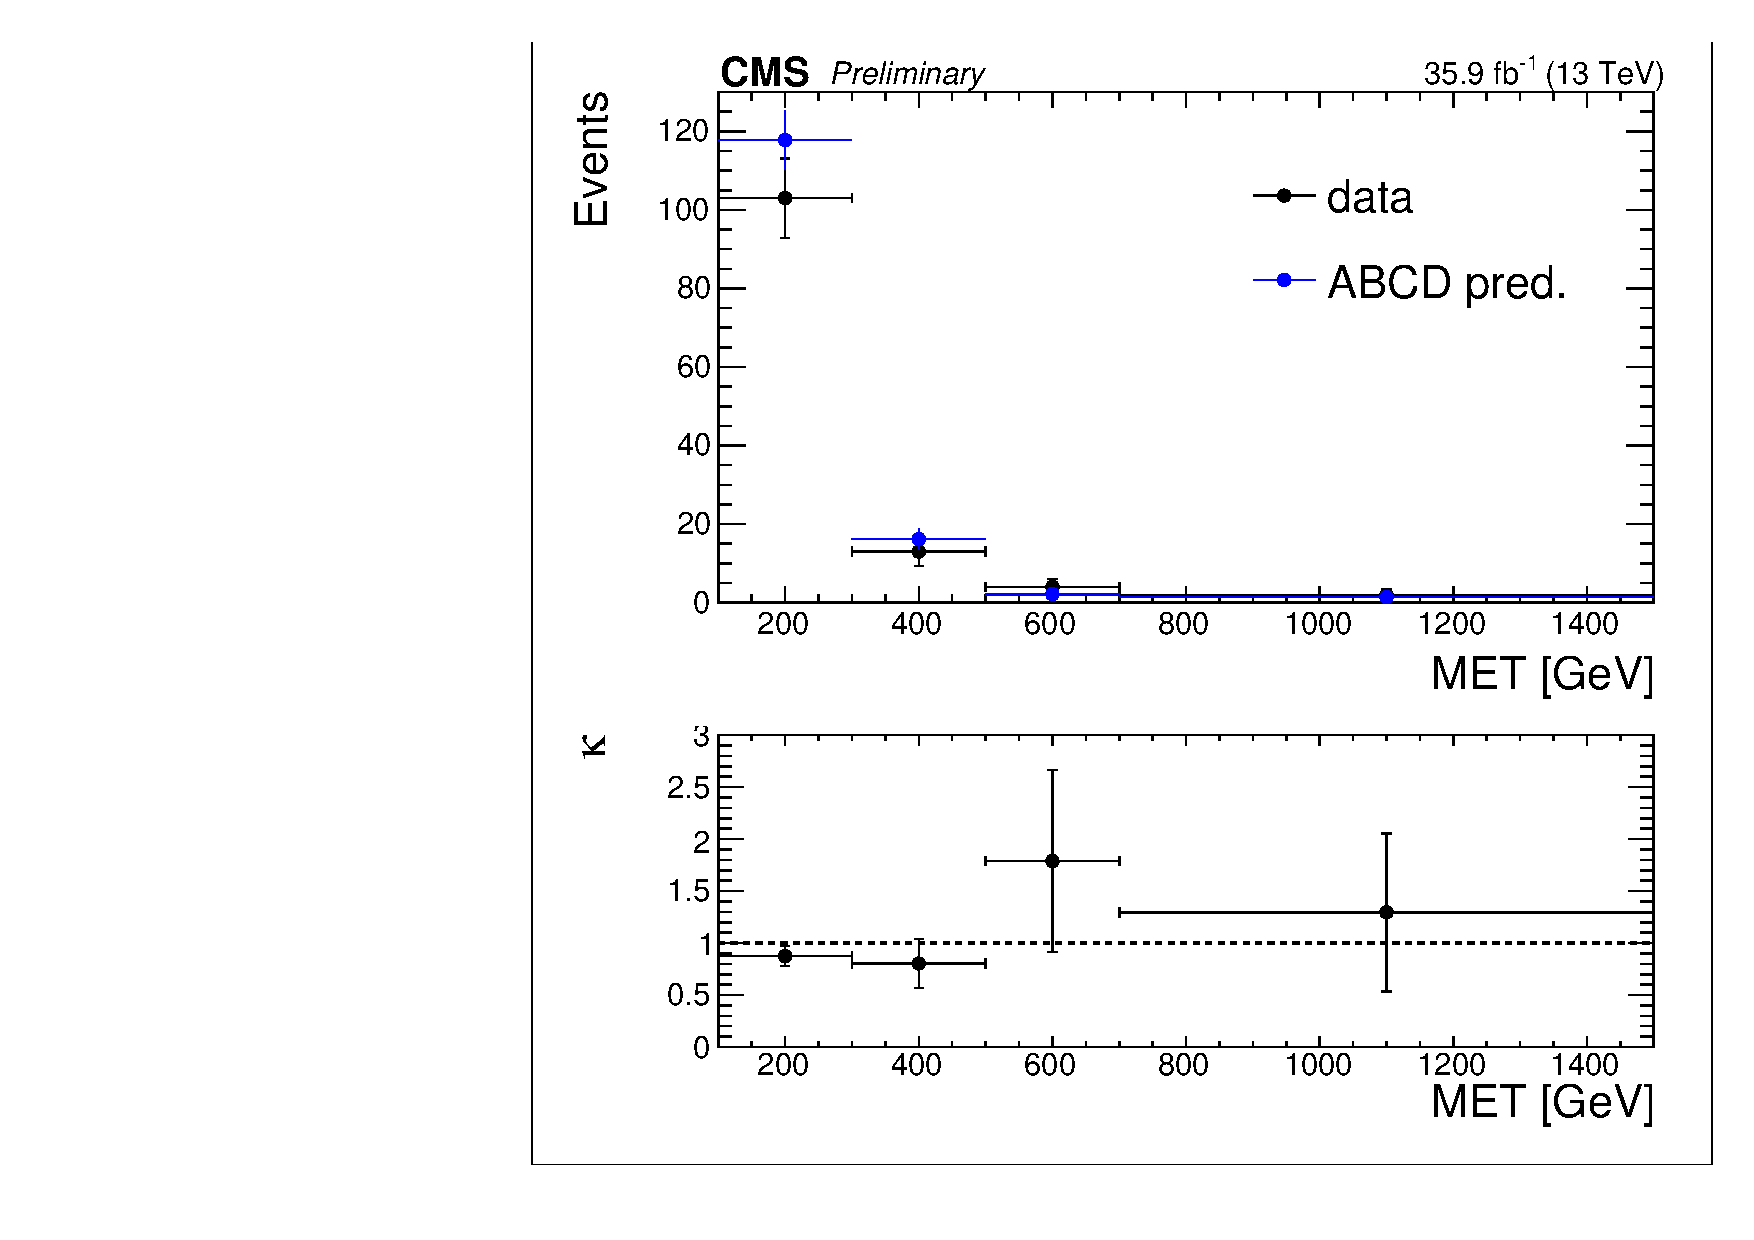
\includegraphics[trim={5px 5px 5px 5px},clip,width=0.95\textwidth]{figs/dataClosure_single-tagSR_photon.pdf}
\caption{single photon A$_{1}$}
\end{subfigure}
\begin{subfigure}[b]{0.425\textwidth}
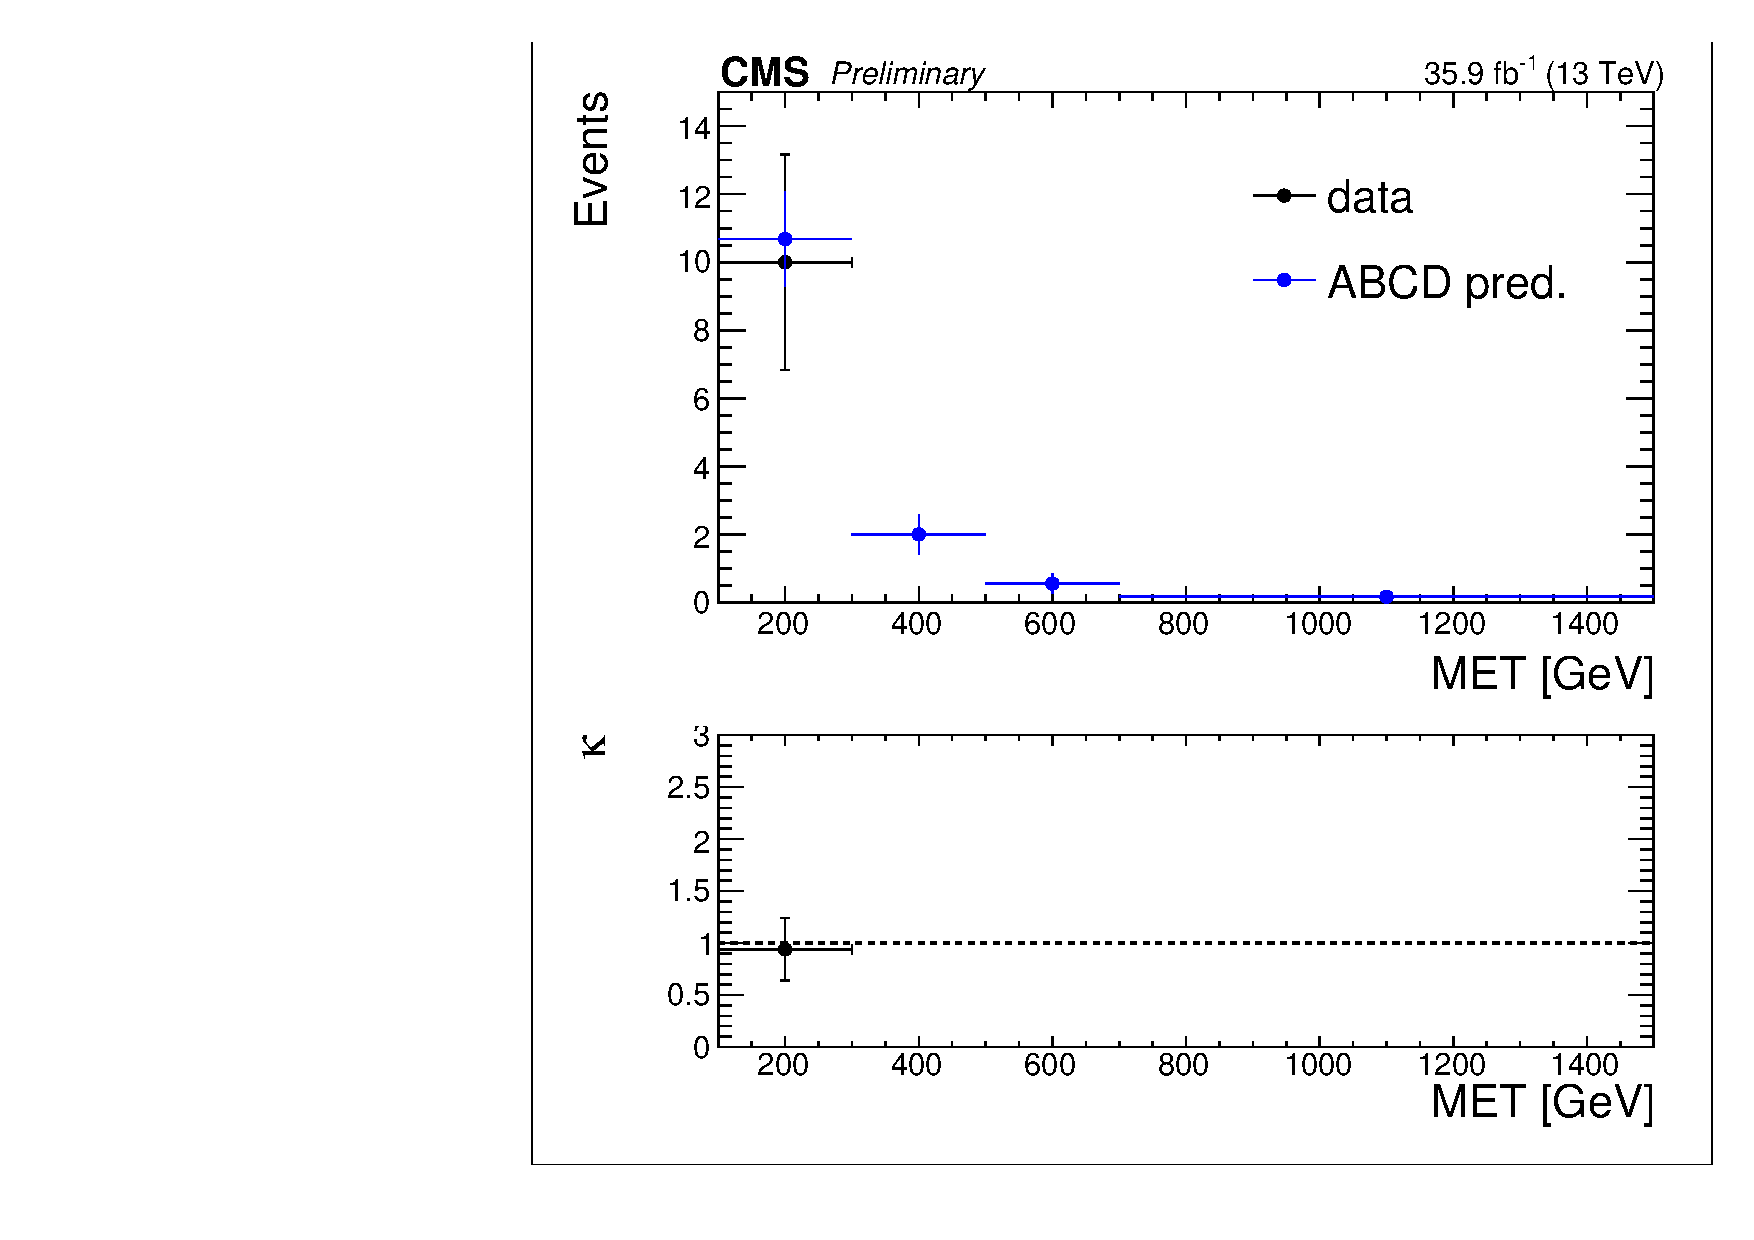
\includegraphics[trim={5px 5px 5px 5px},clip,width=0.95\textwidth]{figs/dataClosure_double-tagSR_photon.pdf} 
\caption{single photon A$_{2}$}
\end{subfigure}
\vspace{5mm}
\\
\begin{subfigure}[b]{0.425\textwidth}
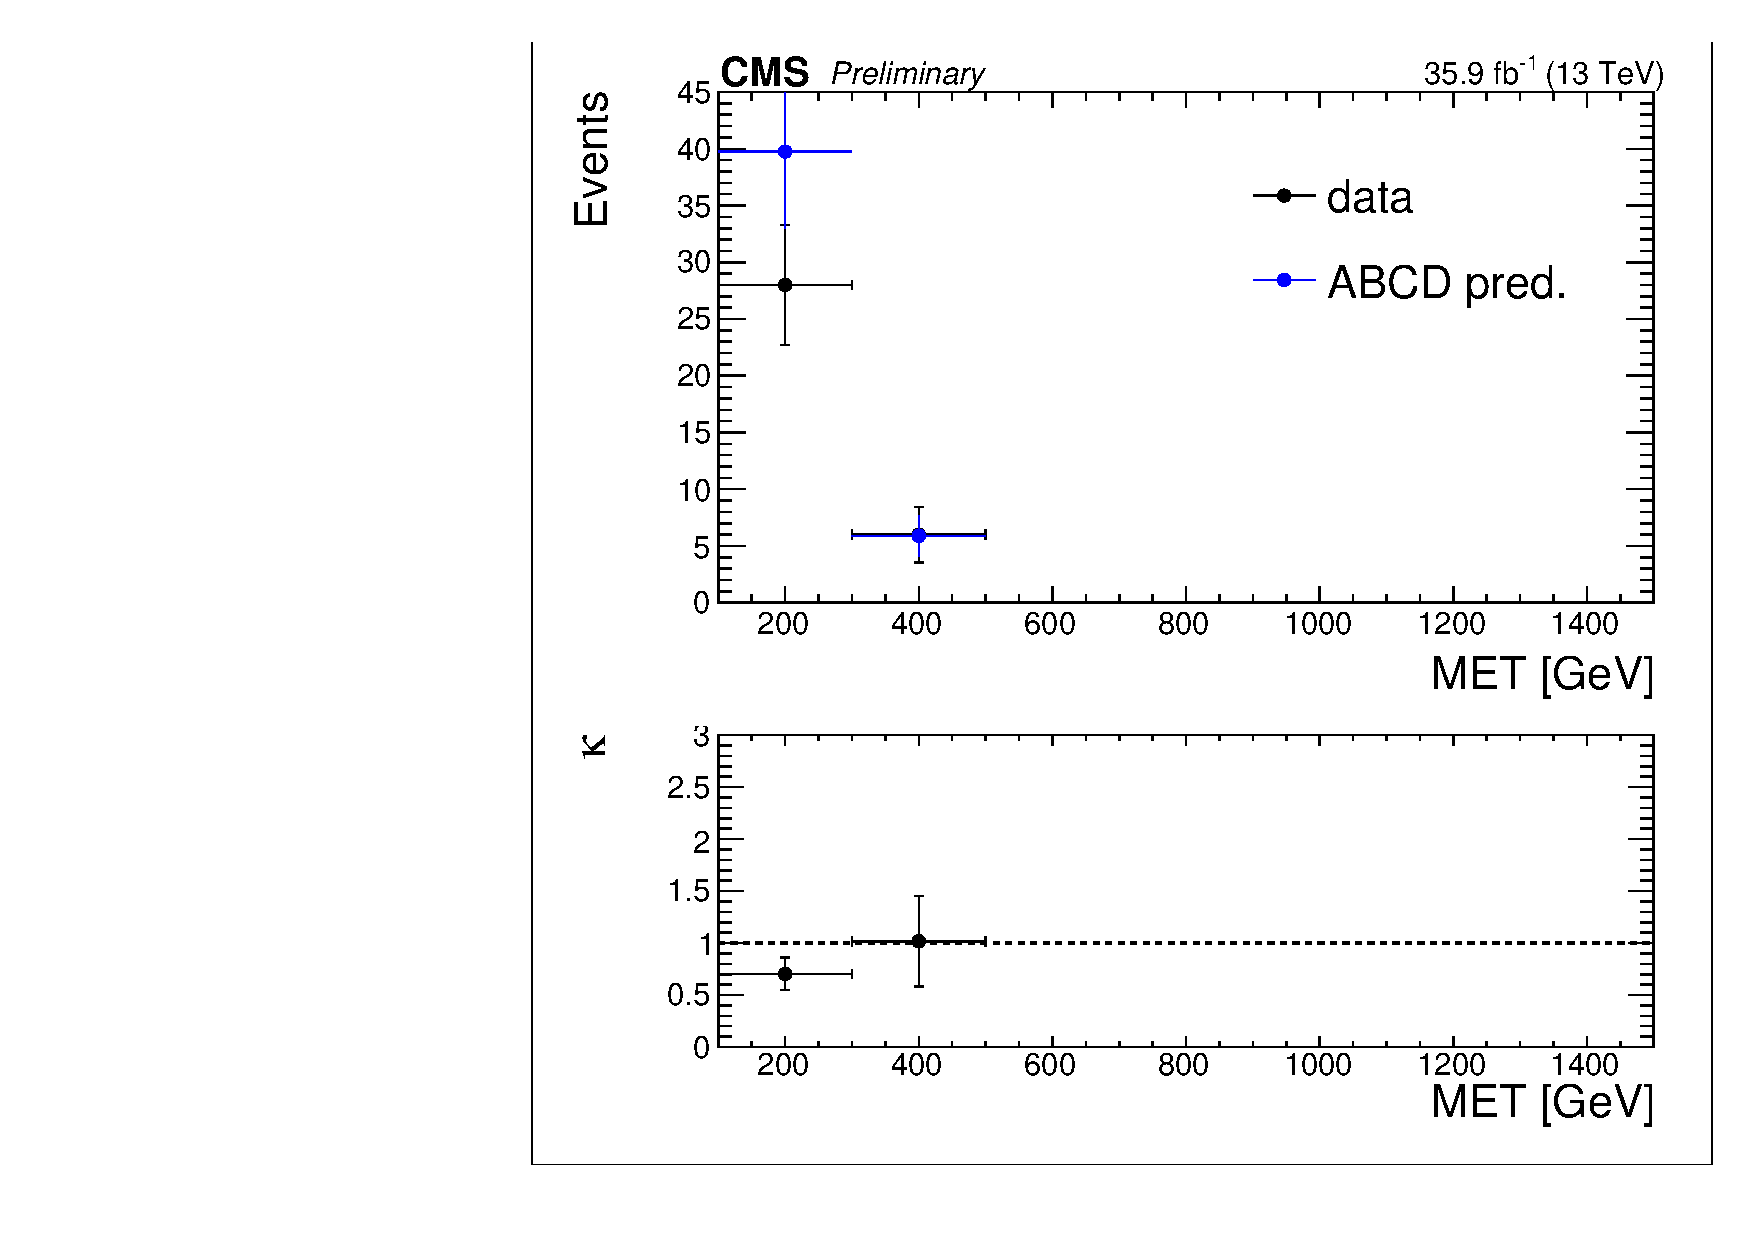
\includegraphics[trim={5px 5px 5px 5px},clip,width=0.95\textwidth]{figs/dataClosure_single-tagSR_singleLep.pdf} 
\caption{single lepton A$_{1}$}
\end{subfigure}
\begin{subfigure}[b]{0.425\textwidth}
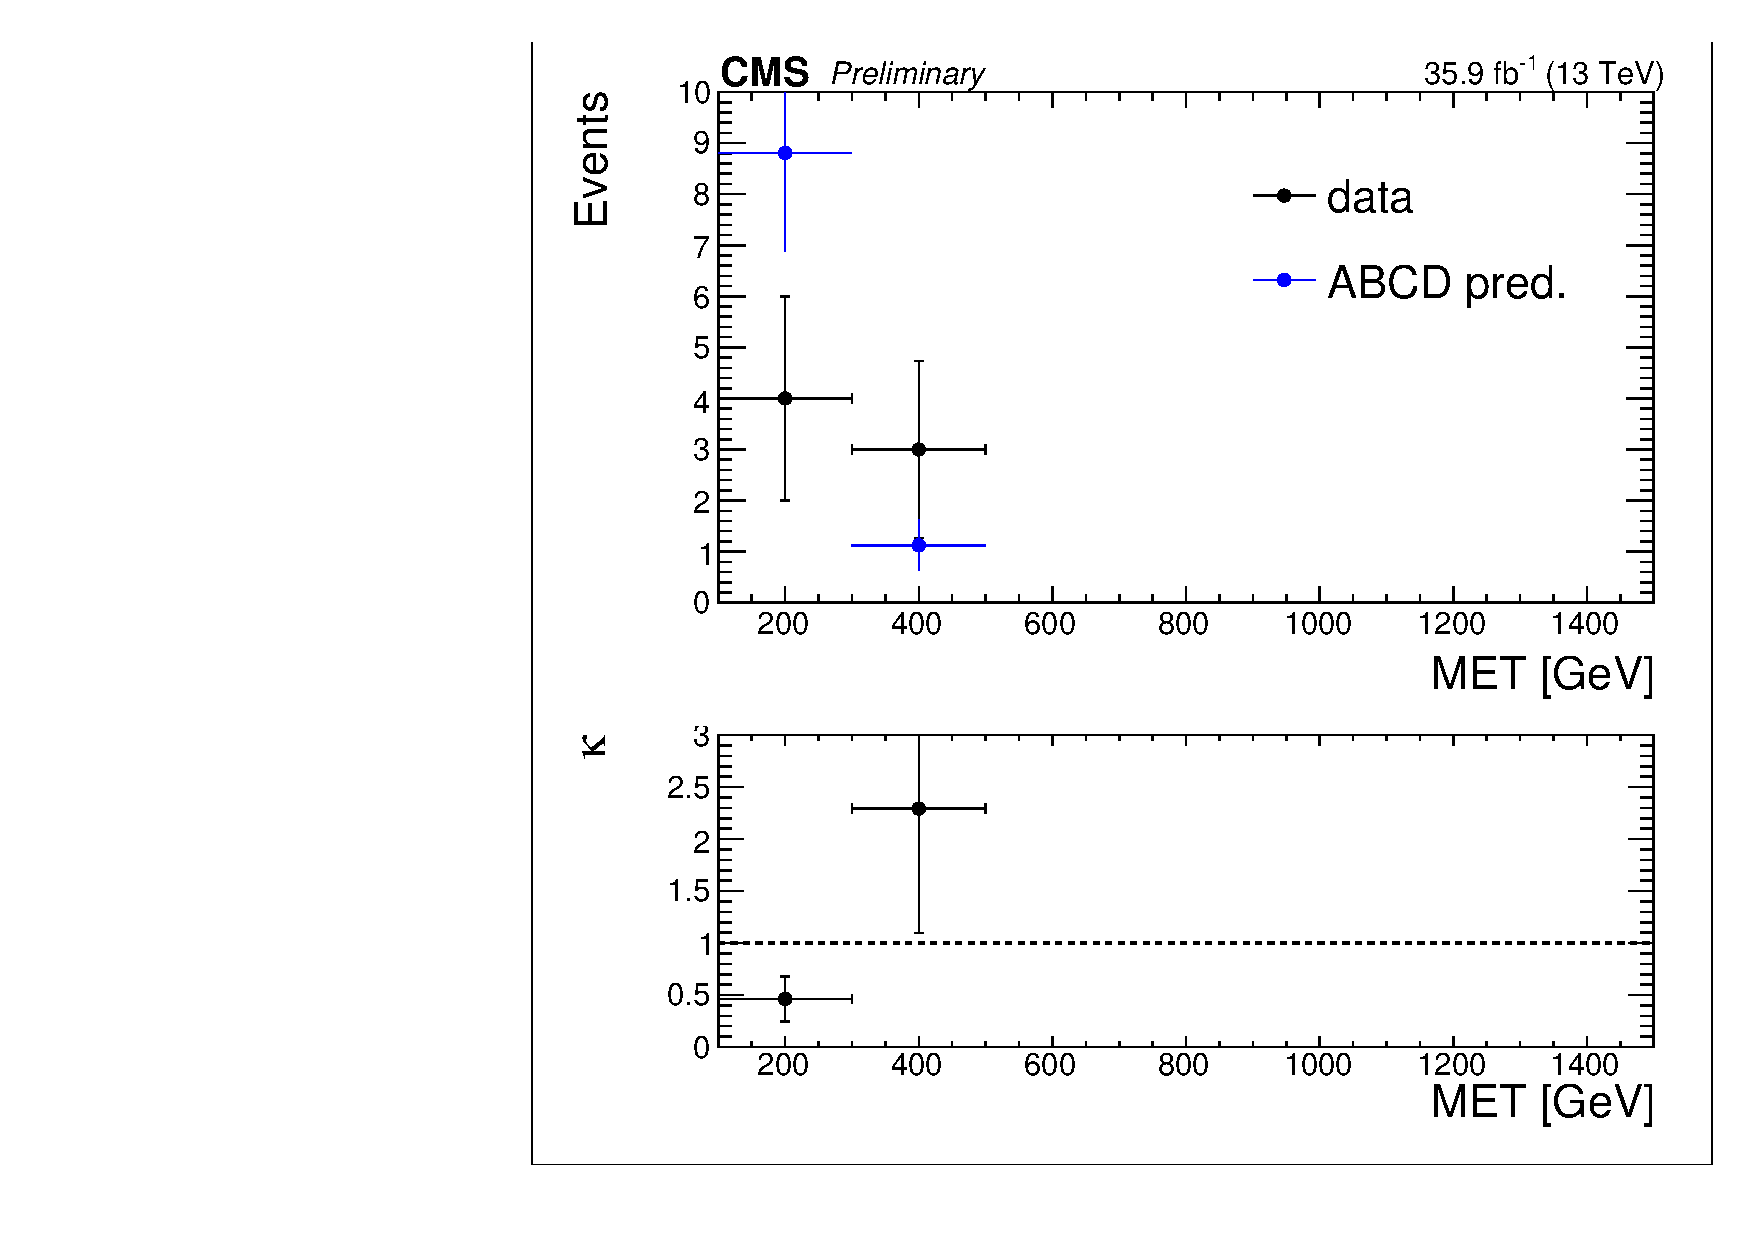
\includegraphics[trim={5px 5px 5px 5px},clip,width=0.95\textwidth]{figs/dataClosure_double-tagSR_singleLep.pdf} 
\caption{single lepton A$_{2}$}
\end{subfigure}
\vspace{5mm}
\\
\begin{subfigure}[b]{0.42\textwidth}
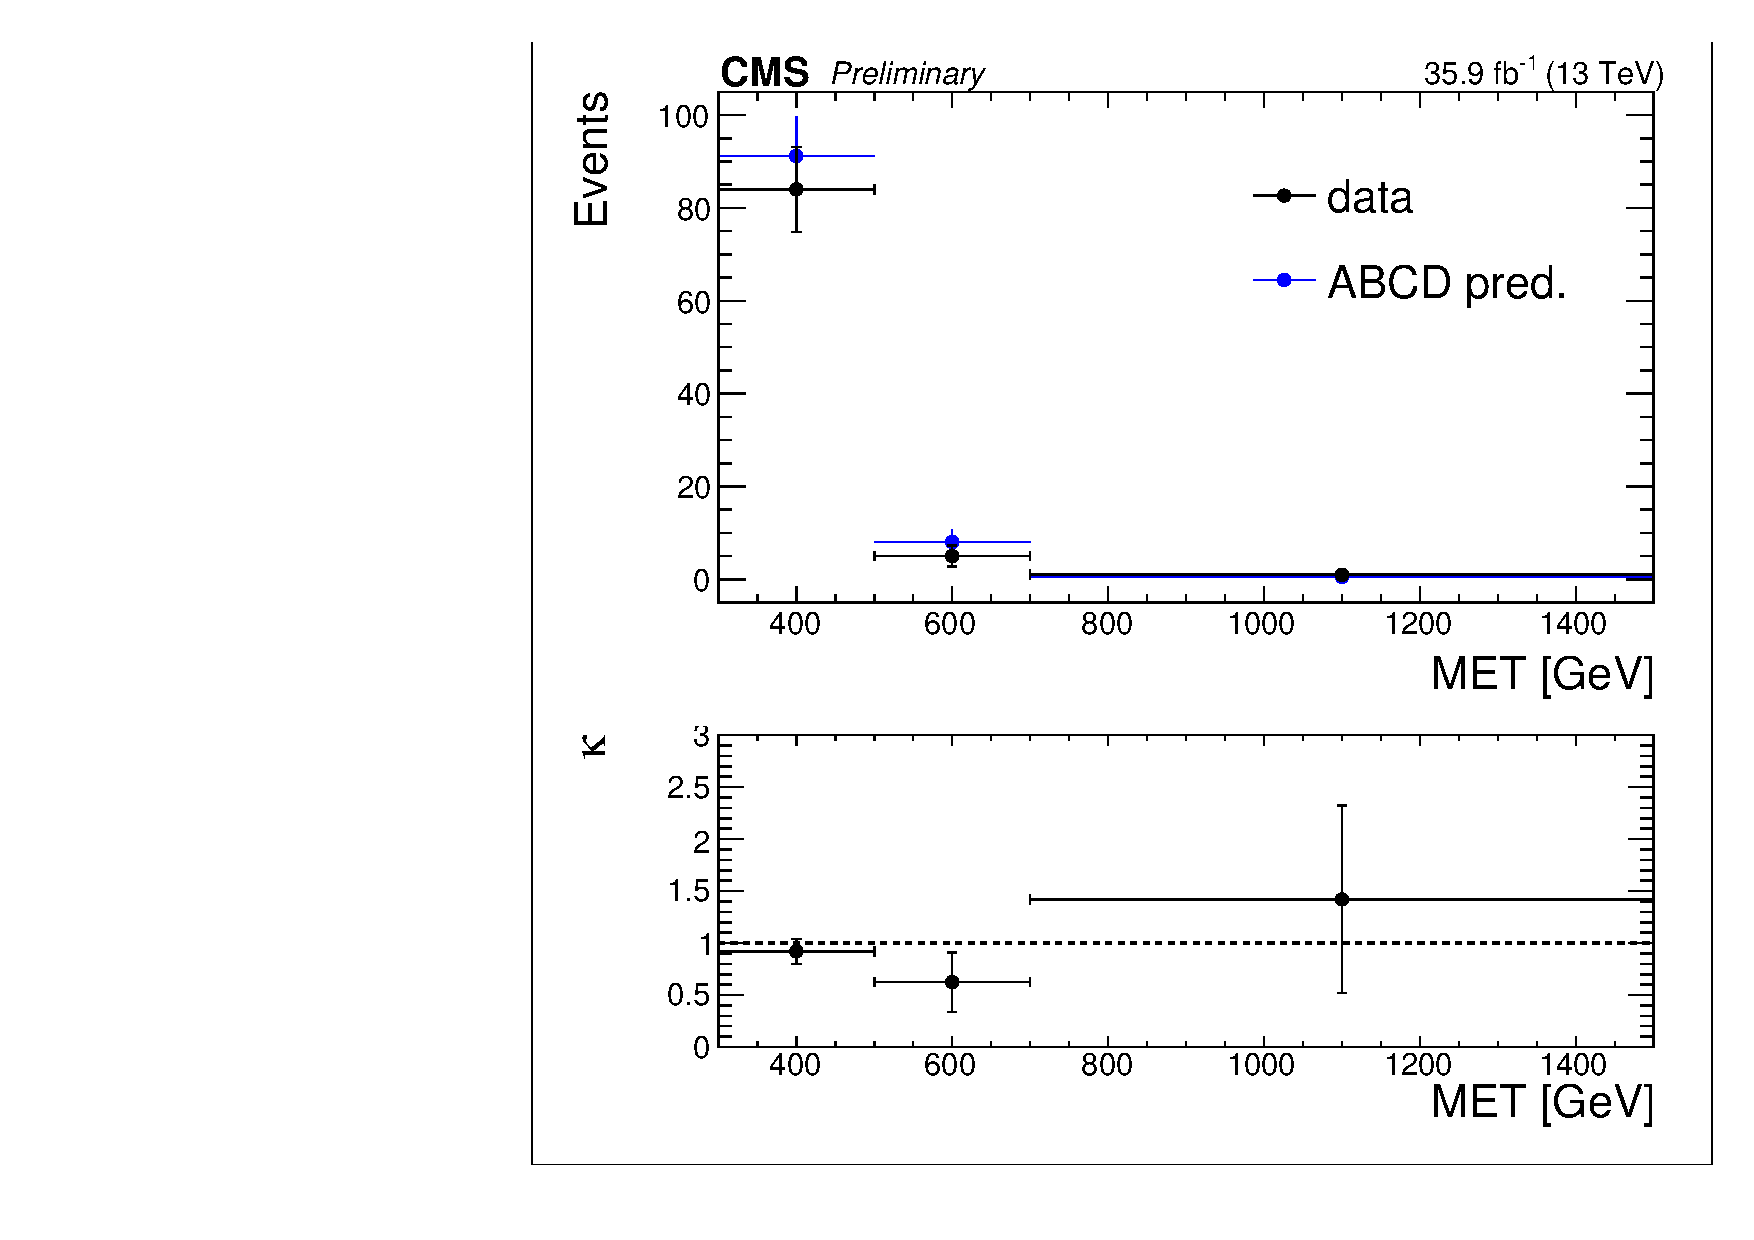
\includegraphics[trim={5px 5px 5px 5px},clip,width=0.95\textwidth]{figs/dataClosure_single-tagSR_lowDphi.pdf} 
\caption{low-$\Delta\phi$ A$_{1}$}
\end{subfigure}
\begin{subfigure}[b]{0.42\textwidth}
\centering
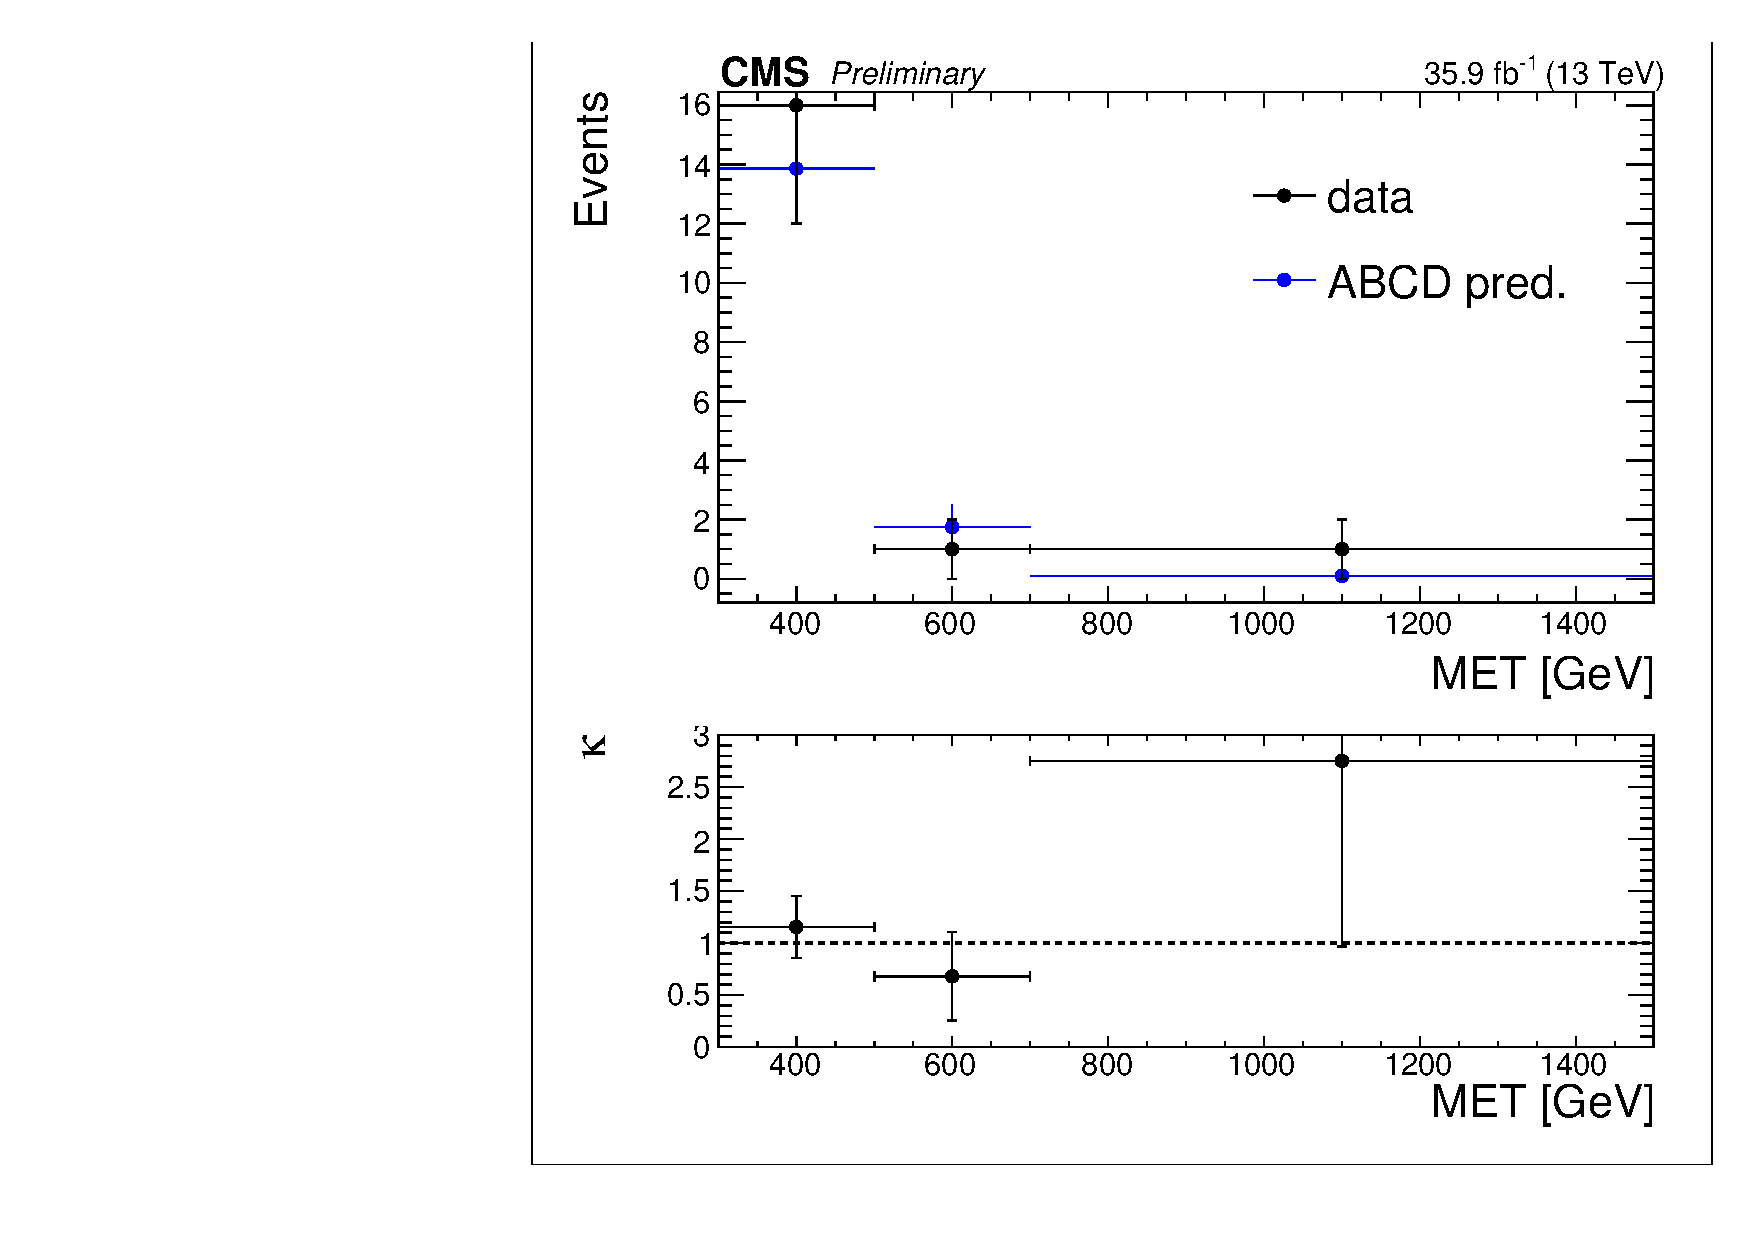
\includegraphics[trim={5px 5px 5px 5px},clip,width=0.95\textwidth]{figs/dataClosure_double-tagSR_lowDphi.pdf} 
\caption{low-$\Delta\phi$ A$_{2}$}
\end{subfigure}
\caption{Comparisons of the predicted and observed yields within the data control regions.}
\label{fig:closure}
\end{figure}

\subsection{$\kappa$ as a Correction to the Estimation}
\label{sec:kappa}

A correction factor $\kappa$ is applied to the prediction to account for the under-prediction of the background estimation procedure as observed in Figure~\ref{fig:mcclosure}. $\kappa$ is obtained by dividing the MC yields for the signal region by that predicted:

\begin{equation}
\kappa  \equiv A^{mc} \,/  \ \left(B \cdot \frac{C} {D} \ \right)^{mc}
\label{eq:kappa}
\end{equation}

There are 2x3=6 values of $\kappa$, one for each signal bin. $\kappa=1$ represents the case of a perfect prediction. The corrections are then applied as follows:

\begin{equation}
A_{1, 2}^{\mathrm{predicted}} = \kappa \cdot \left(B_{1, 2} \cdot \ \frac{C}{D}\right)^{\textrm{observed}}
\end{equation}

These values of $\kappa$ are those which we have already seen in Figure~\ref{fig:mcclosure}.

The value of $\kappa$ is dependent on the yields of each analysis bin and is therefore sensitive to the accuracy of the modeling of MC in each of the 18 analysis bins. To improve the determination of $\kappa$, scale factors are derived using the data control regions to correct the normalization of MC in each of these bins. Different scale factors are assigned separately to the Z-invisible, lost-lepton, and QCD background MC samples. Rare processes (e.g. diboson) are taken directly from MC.

First consider how the yield N predicted by MC in an arbitrary bin (of 18) is the sum of the yields in the different MC datasets ($t\bar{t}$ and $W\rightarrow\ell\nu$ are grouped as they together represent the lost-lepton background):

\begin{equation}
N^{mc} = N_{Z\rightarrow\nu\bar{\nu}}^{mc} + N_{t\bar{t},\,W\rightarrow\ell\nu}^{mc} + N_{QCD}^{mc} + N_{rare}
\end{equation}

Scale factors are defined for this bin using the corresponding control regions in data and forming the ratio of events in simulation to that observed. They are then applied as follows:

\begin{equation}
N_{corrected}^{mc} = \left(\frac{N_{single-\gamma}^{data}}{N_{single-\gamma}^{mc}}\right) \cdot N_{Z\rightarrow\nu\bar{\nu}}^{mc} + \left(\frac{N^{data}_{single-\ell}}{N^{mc}_{single-\ell}}\right) \cdot N^{mc}_{t\bar{t},\,W\rightarrow\ell\nu} + \left(\frac{N^{data}_{low-\Delta\phi}}{N^{mc}_{low-\Delta\phi}}\right) \cdot N_{QCD}^{mc} + N_{rare}
\end{equation}

The \ptmiss distribution within the control regions is shown for both data and MC in Figures~\ref{fig:closurephoton},~\ref{fig:closuresinglelep},~\ref{fig:closurelowdphi} for the single photon, single lepton, and low-$\Delta\phi$ control regions, respectively. The ratio in the bottom panel of each plot represents the scale factor for that \ptmiss bin. The dotted horizontal line shows the average scale factor inclusive in \ptmiss. The scale factors for the single-photon and low-$\Delta\phi$ control regions show no \ptmiss dependence and are determined integrated over \ptmiss$>300\,\textrm{GeV}$. The values of the scale factors are summarized in Table~\ref{tab:ScaleFactorVR}. The Single-lepton region, shown in Figure~\ref{fig:closuresinglelep}, does show \ptmiss dependence and are summarized in Tables~\ref{tab:ScaleFactorVR}~and~\ref{tab:ScaleFactorMET}.  In order to improve statistics for the single-lepton region, the low-$\Delta\phi$ requirement has been removed.

\begin{figure}[hbp!]
 \centering
 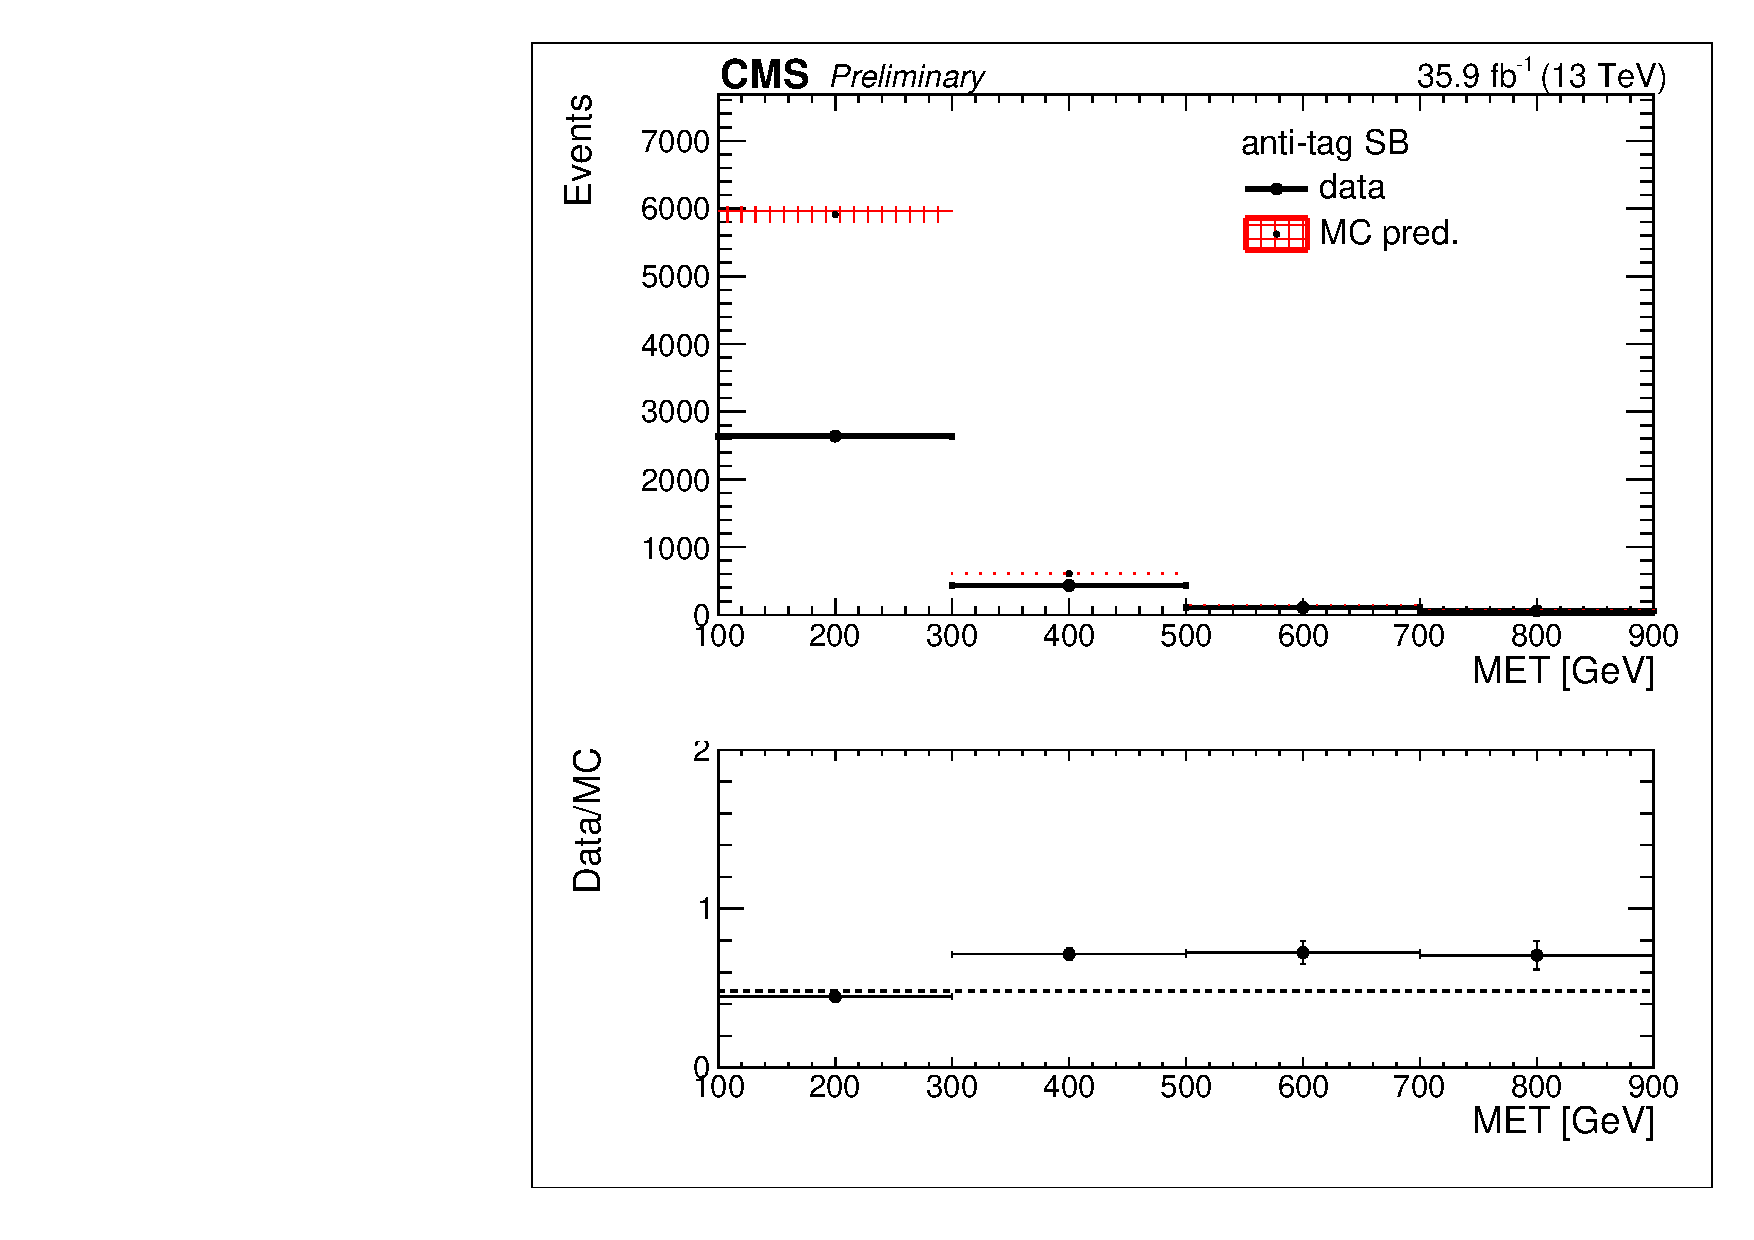
\includegraphics[trim={5px 5px 5px 5px},clip,width=0.425\linewidth]{figs/ABCDscaleFactors_MET_antitagSB_photon.pdf}
 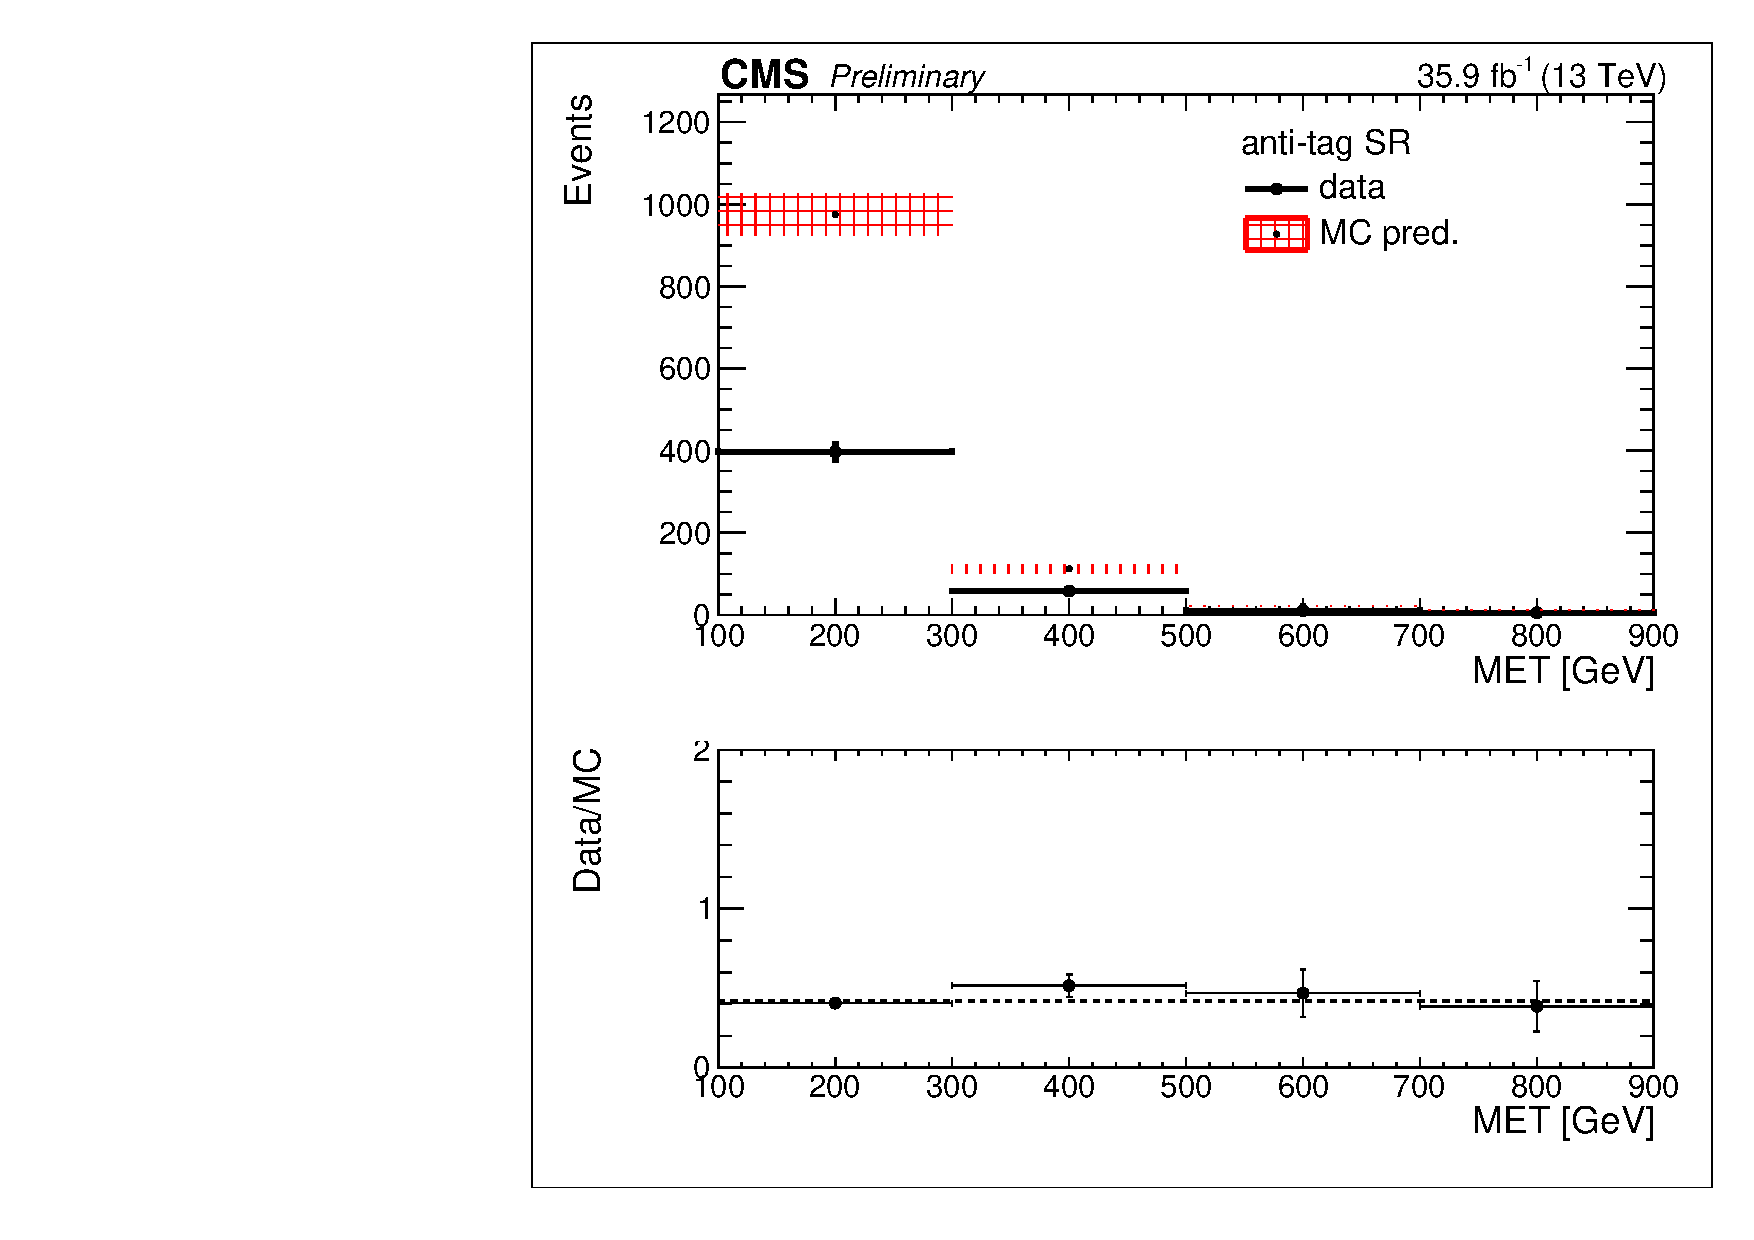
\includegraphics[trim={5px 5px 5px 5px},clip,width=0.425\linewidth]{figs/ABCDscaleFactors_MET_antitagSR_photon.pdf}\\
 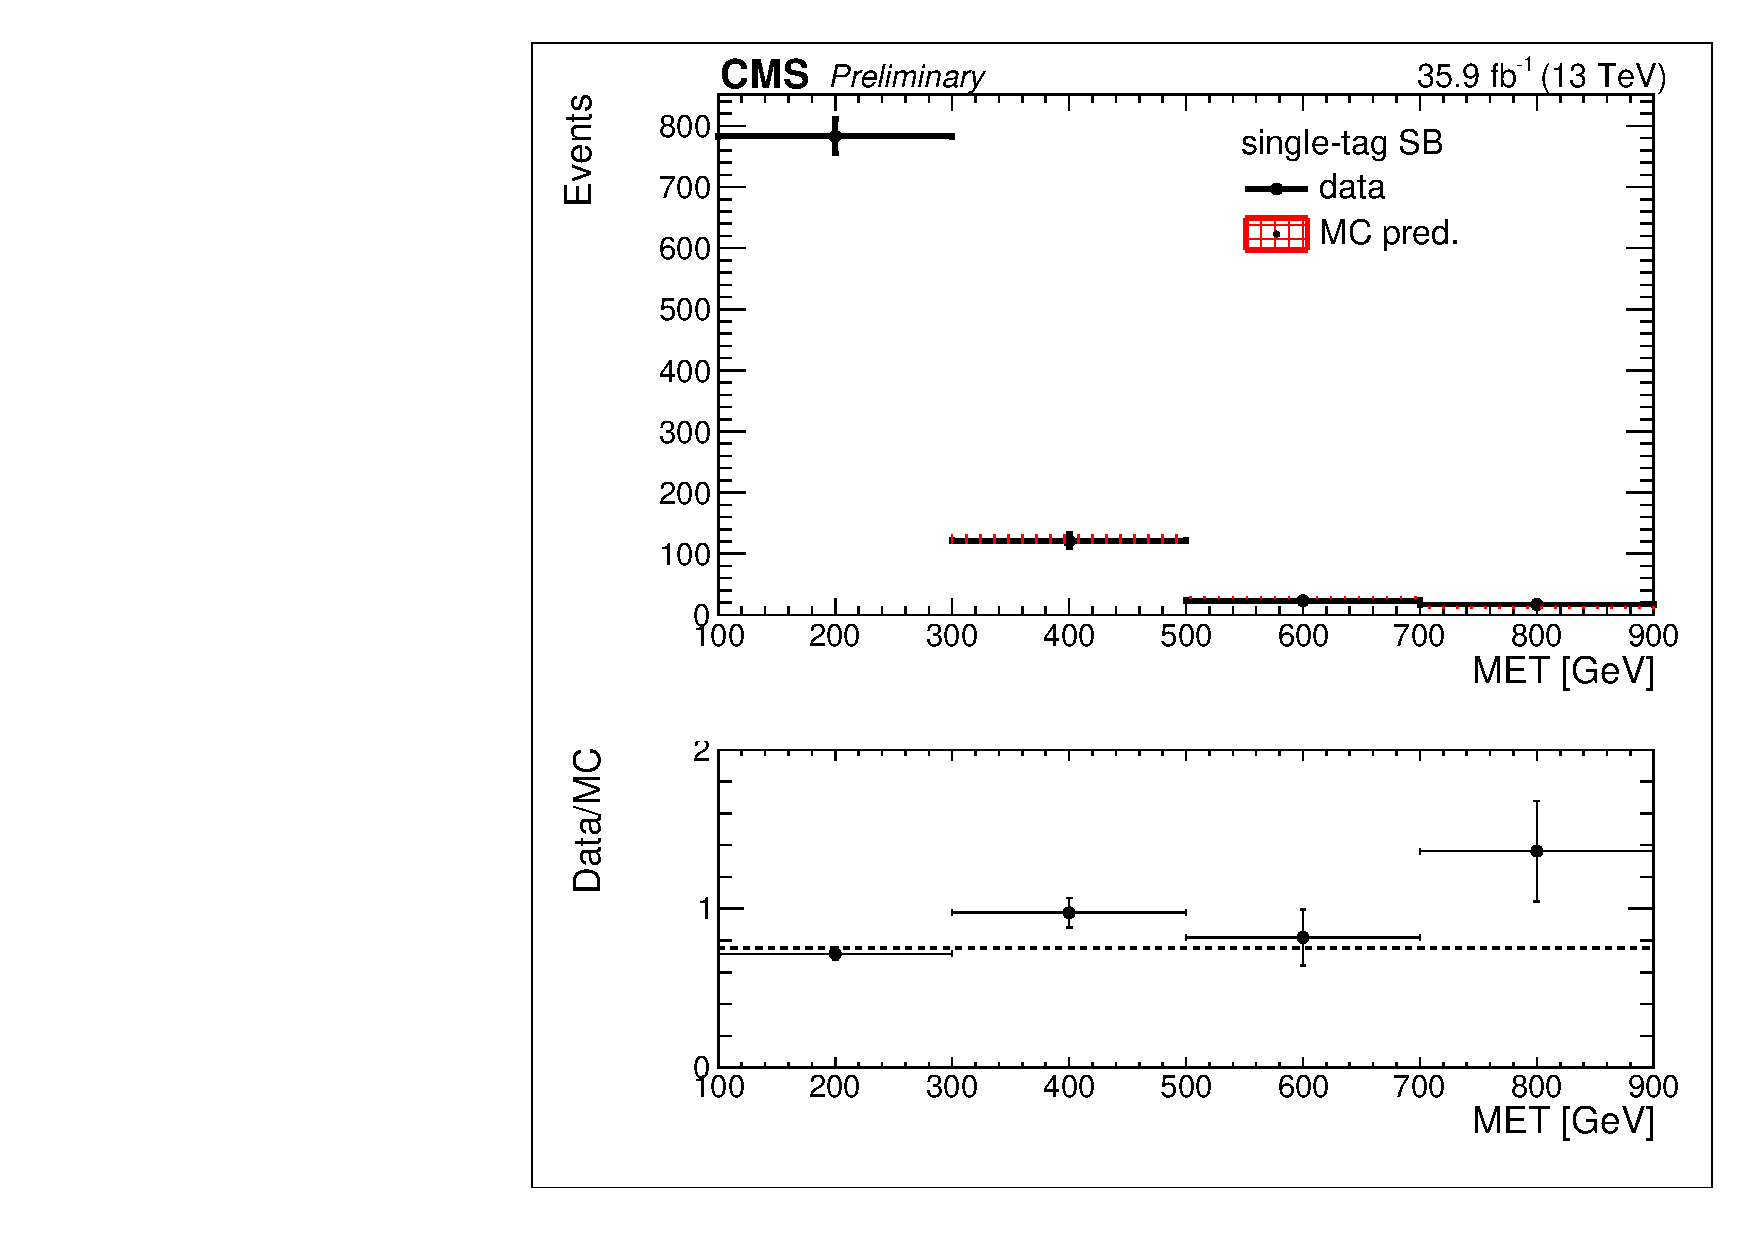
\includegraphics[trim={5px 5px 5px 5px},clip,width=0.425\linewidth]{figs/ABCDscaleFactors_MET_single-tagSB_photon.pdf}
 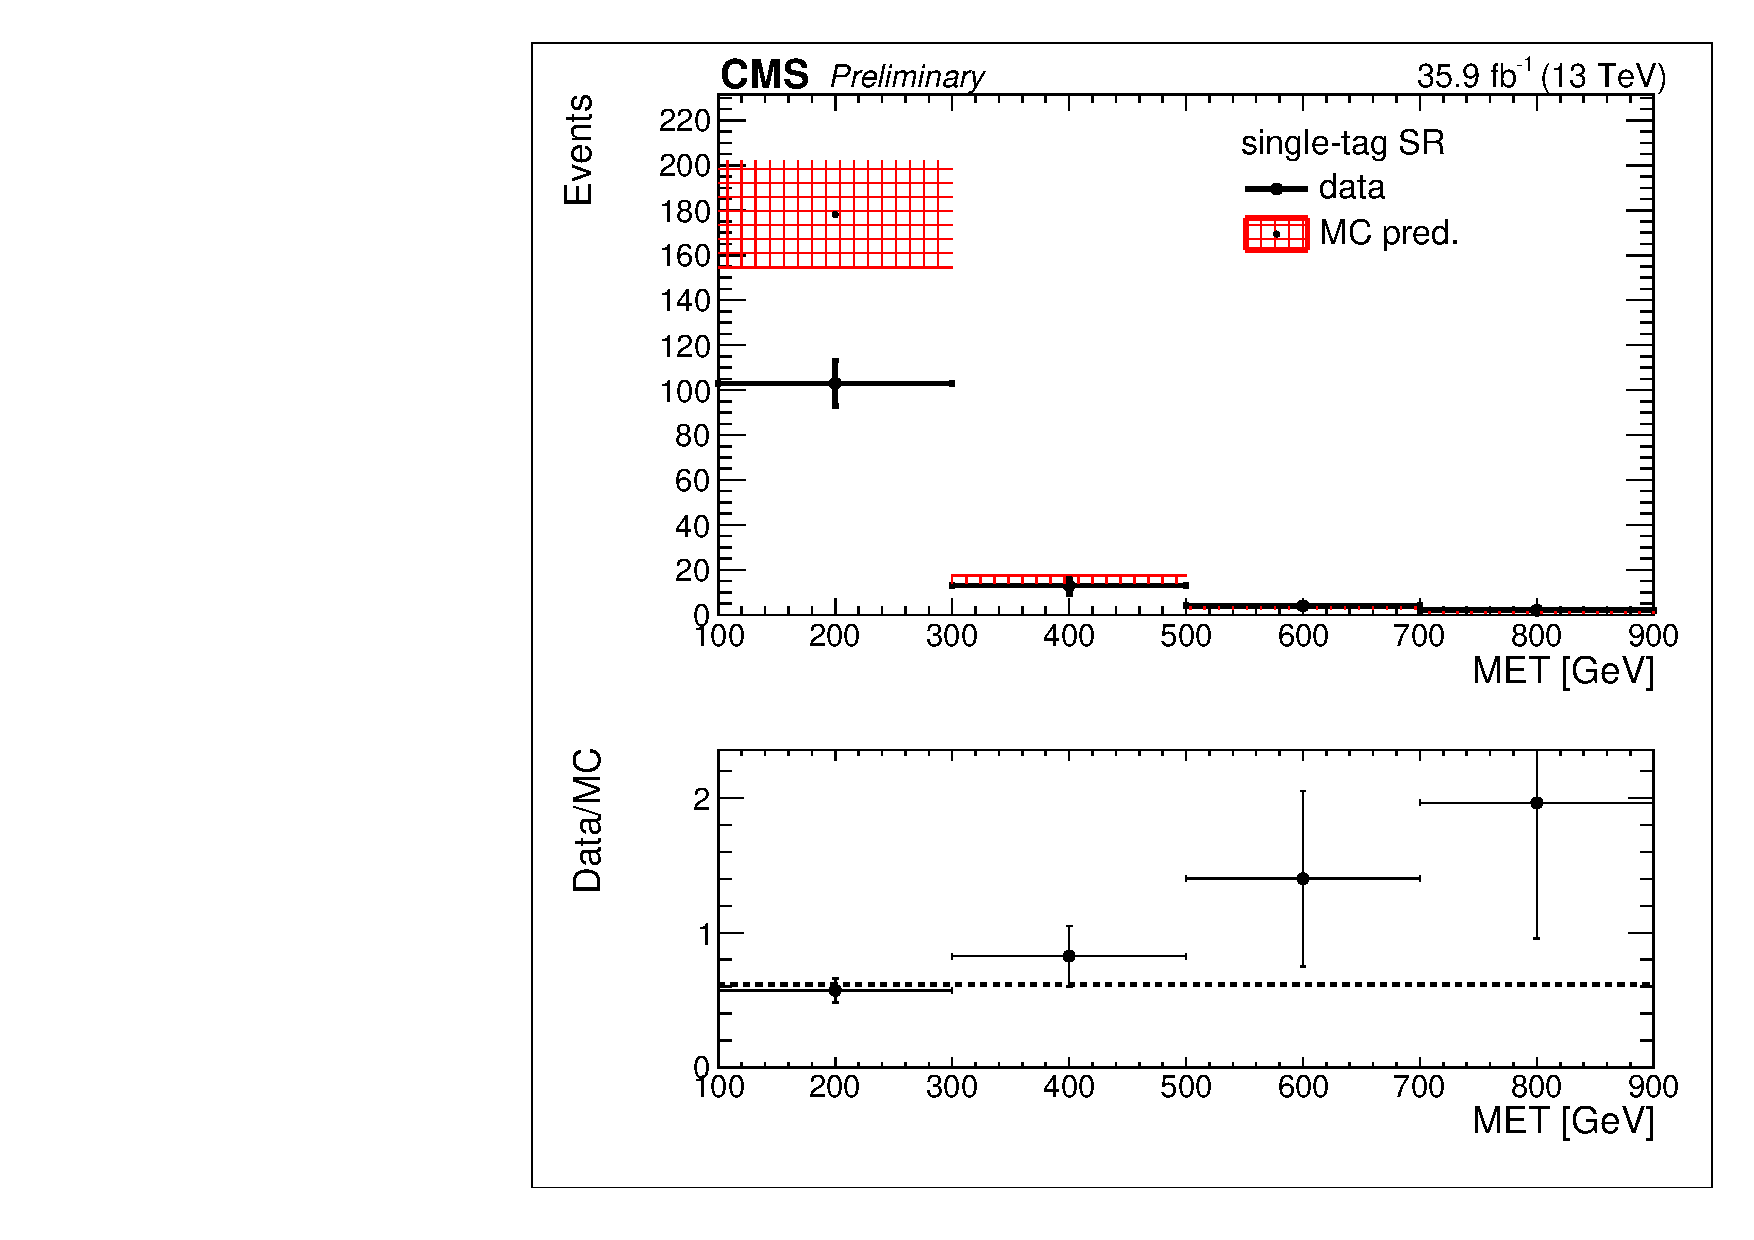
\includegraphics[trim={5px 5px 5px 5px},clip,width=0.425\linewidth]{figs/ABCDscaleFactors_MET_single-tagSR_photon.pdf}\\
 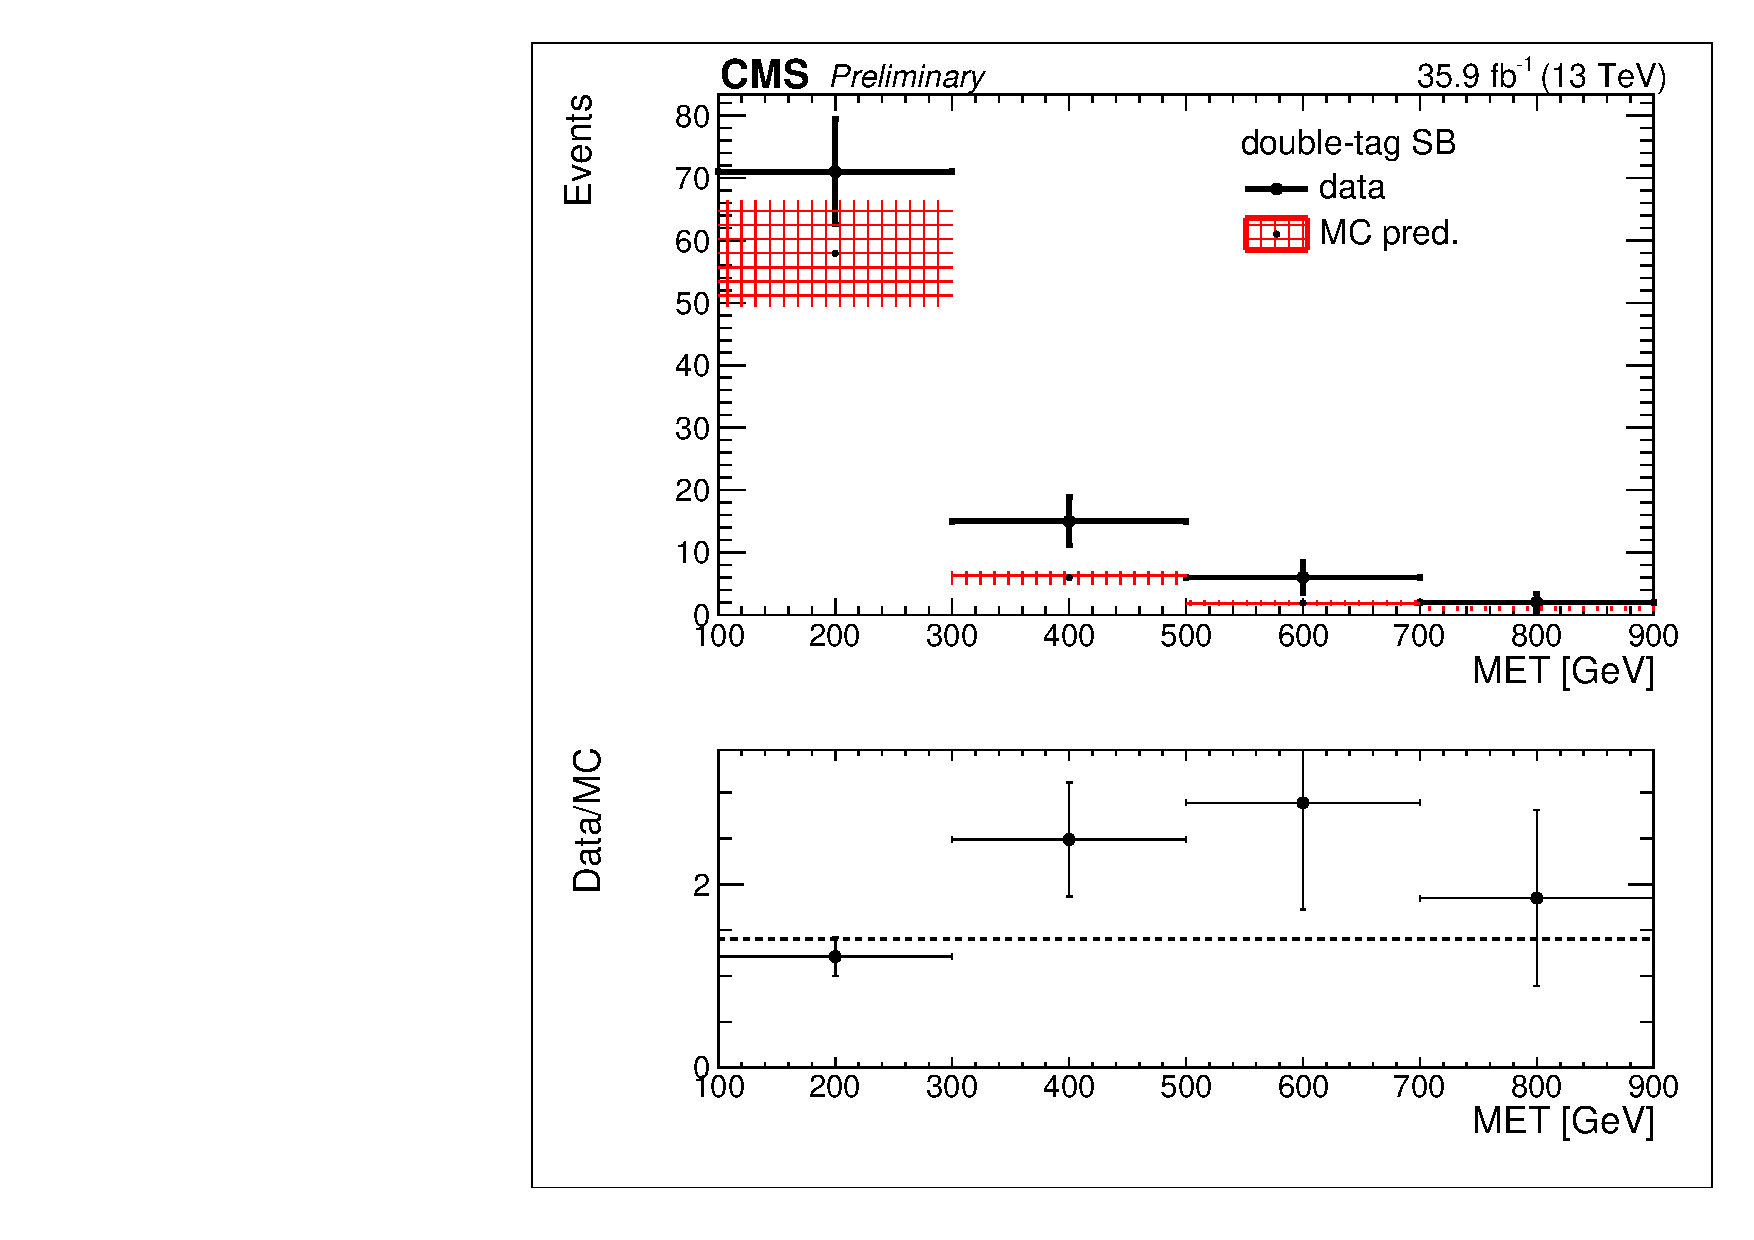
\includegraphics[trim={5px 5px 5px 5px},clip,width=0.425\linewidth]{figs/ABCDscaleFactors_MET_double-tagSB_photon.pdf}
 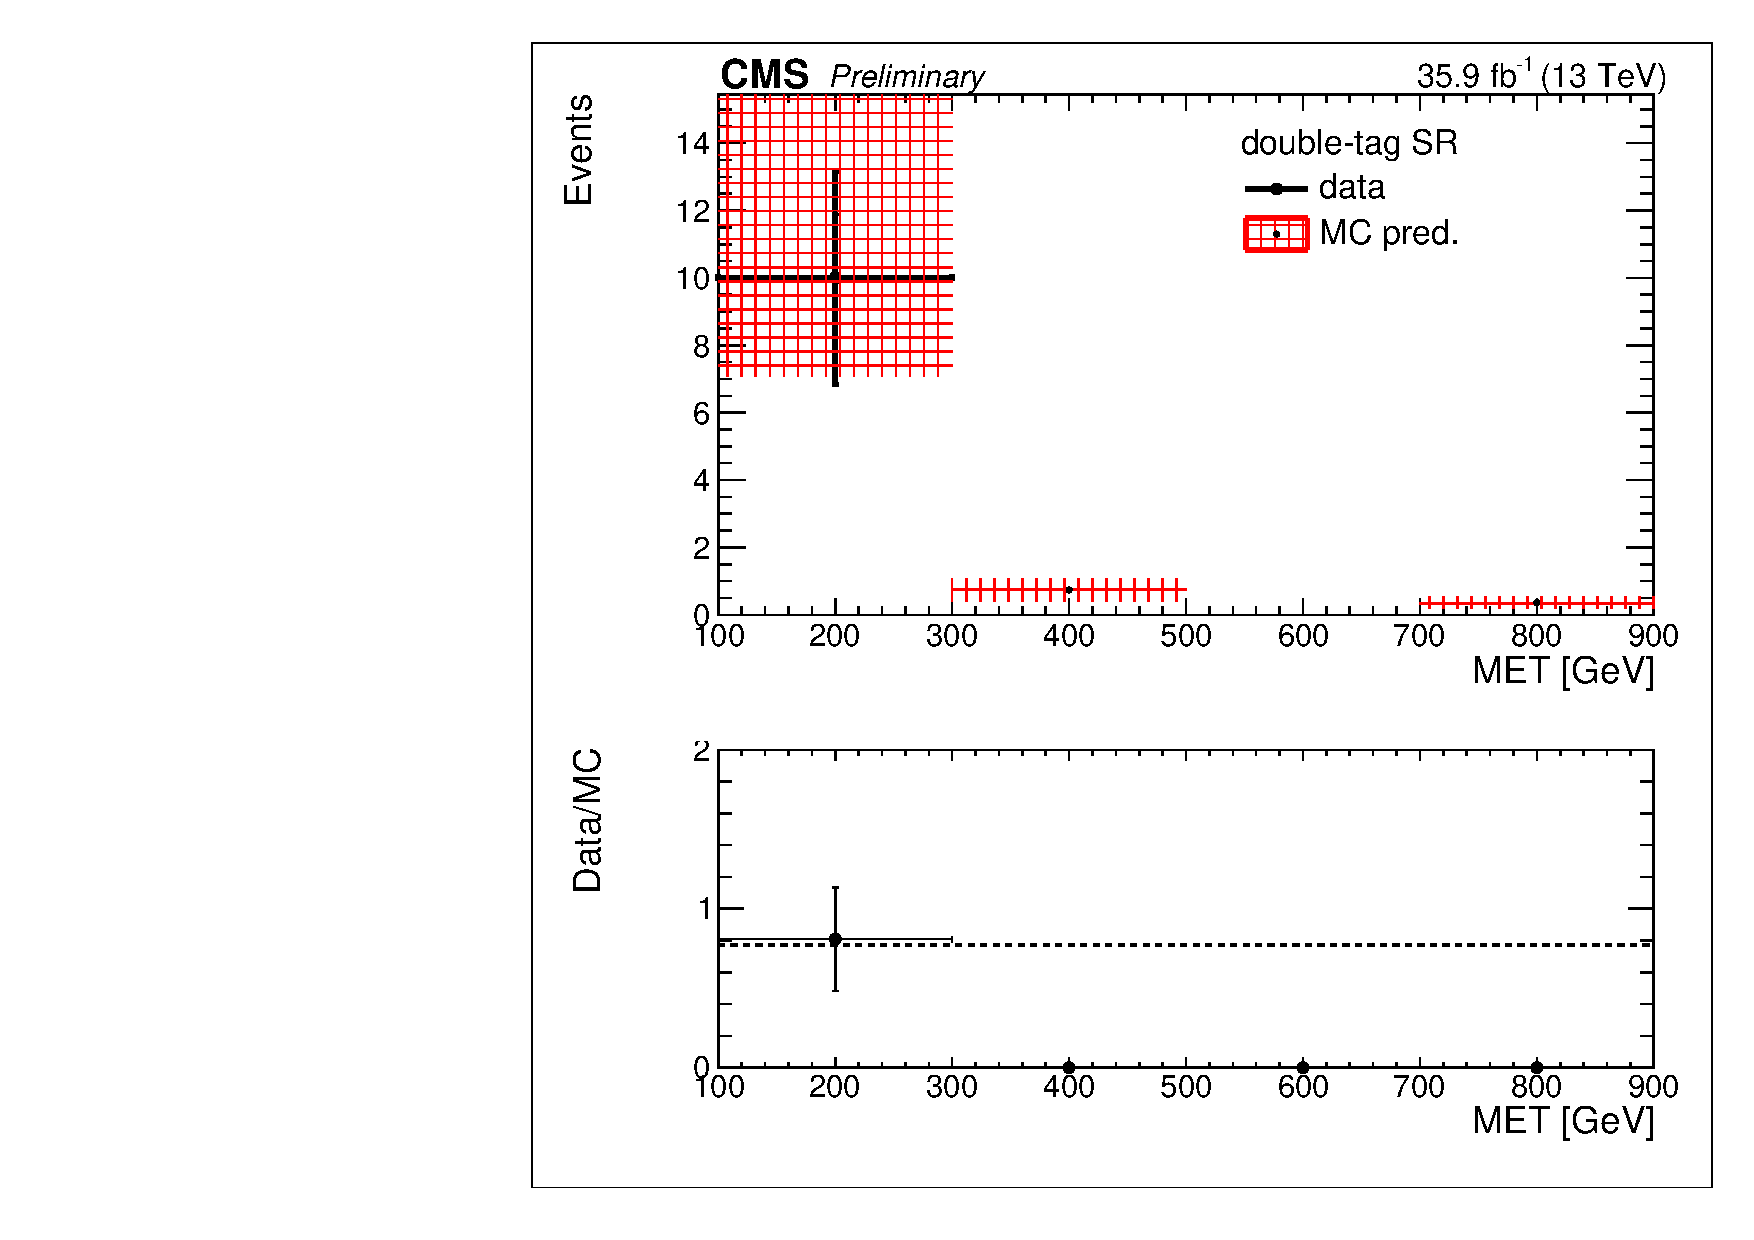
\includegraphics[trim={5px 5px 5px 5px},clip,width=0.425\linewidth]{figs/ABCDscaleFactors_MET_double-tagSR_photon.pdf}\\
 \caption
 [Signal and sideband yields in the single photon control region.]
 {Signal and sideband yields in the single photon control region. The hashed red band denotes the prediction from simulation; the solid black points denote the observed yields in data. The Data/MC ratio in the lower panel of each plot represents the scale factor for that bin. }
\label{fig:closurephoton}
\end{figure}

\begin{figure}[hbp!]
\centering
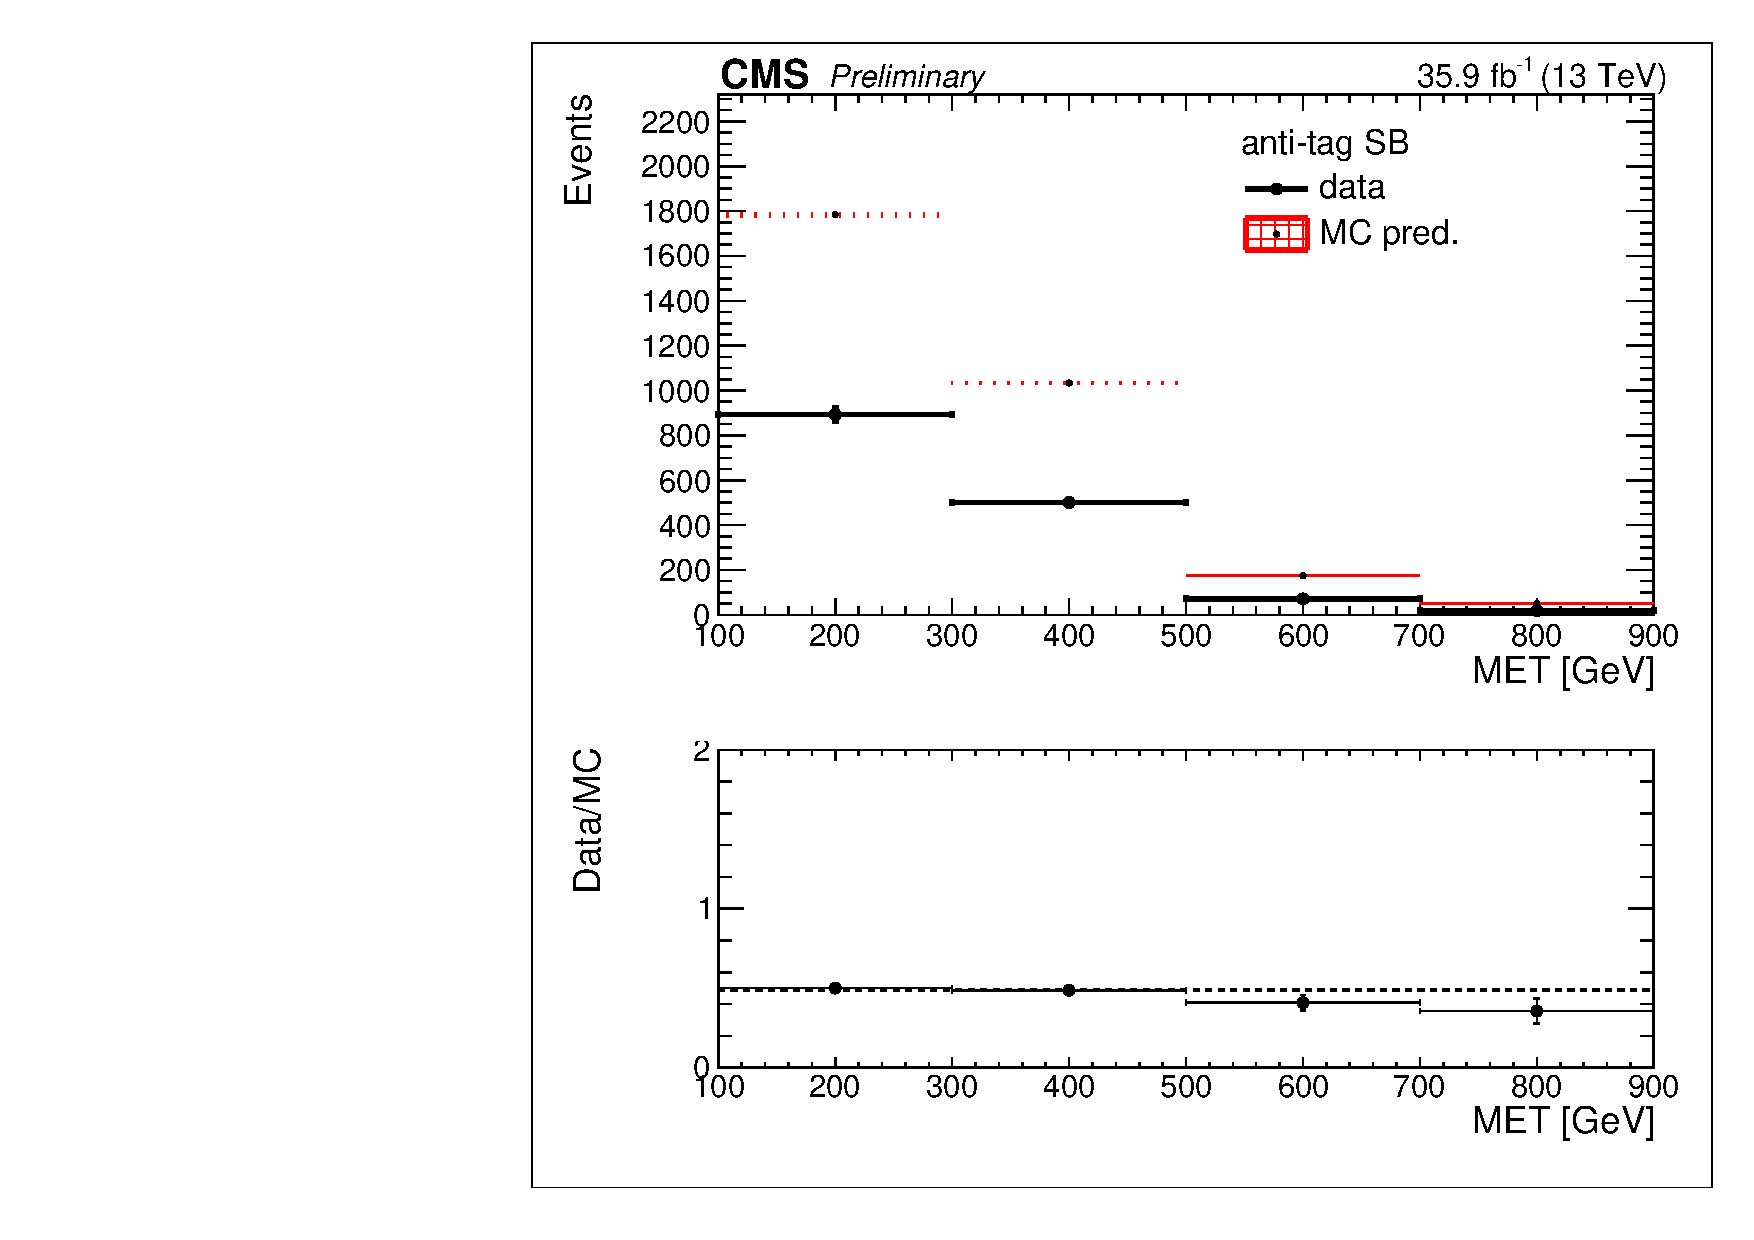
\includegraphics[trim={5px 5px 5px 5px},clip,width=0.425\linewidth]{figs/ABCDscaleFactors_MET_antitagSB_lowDeltaPhi_singleLep.pdf}
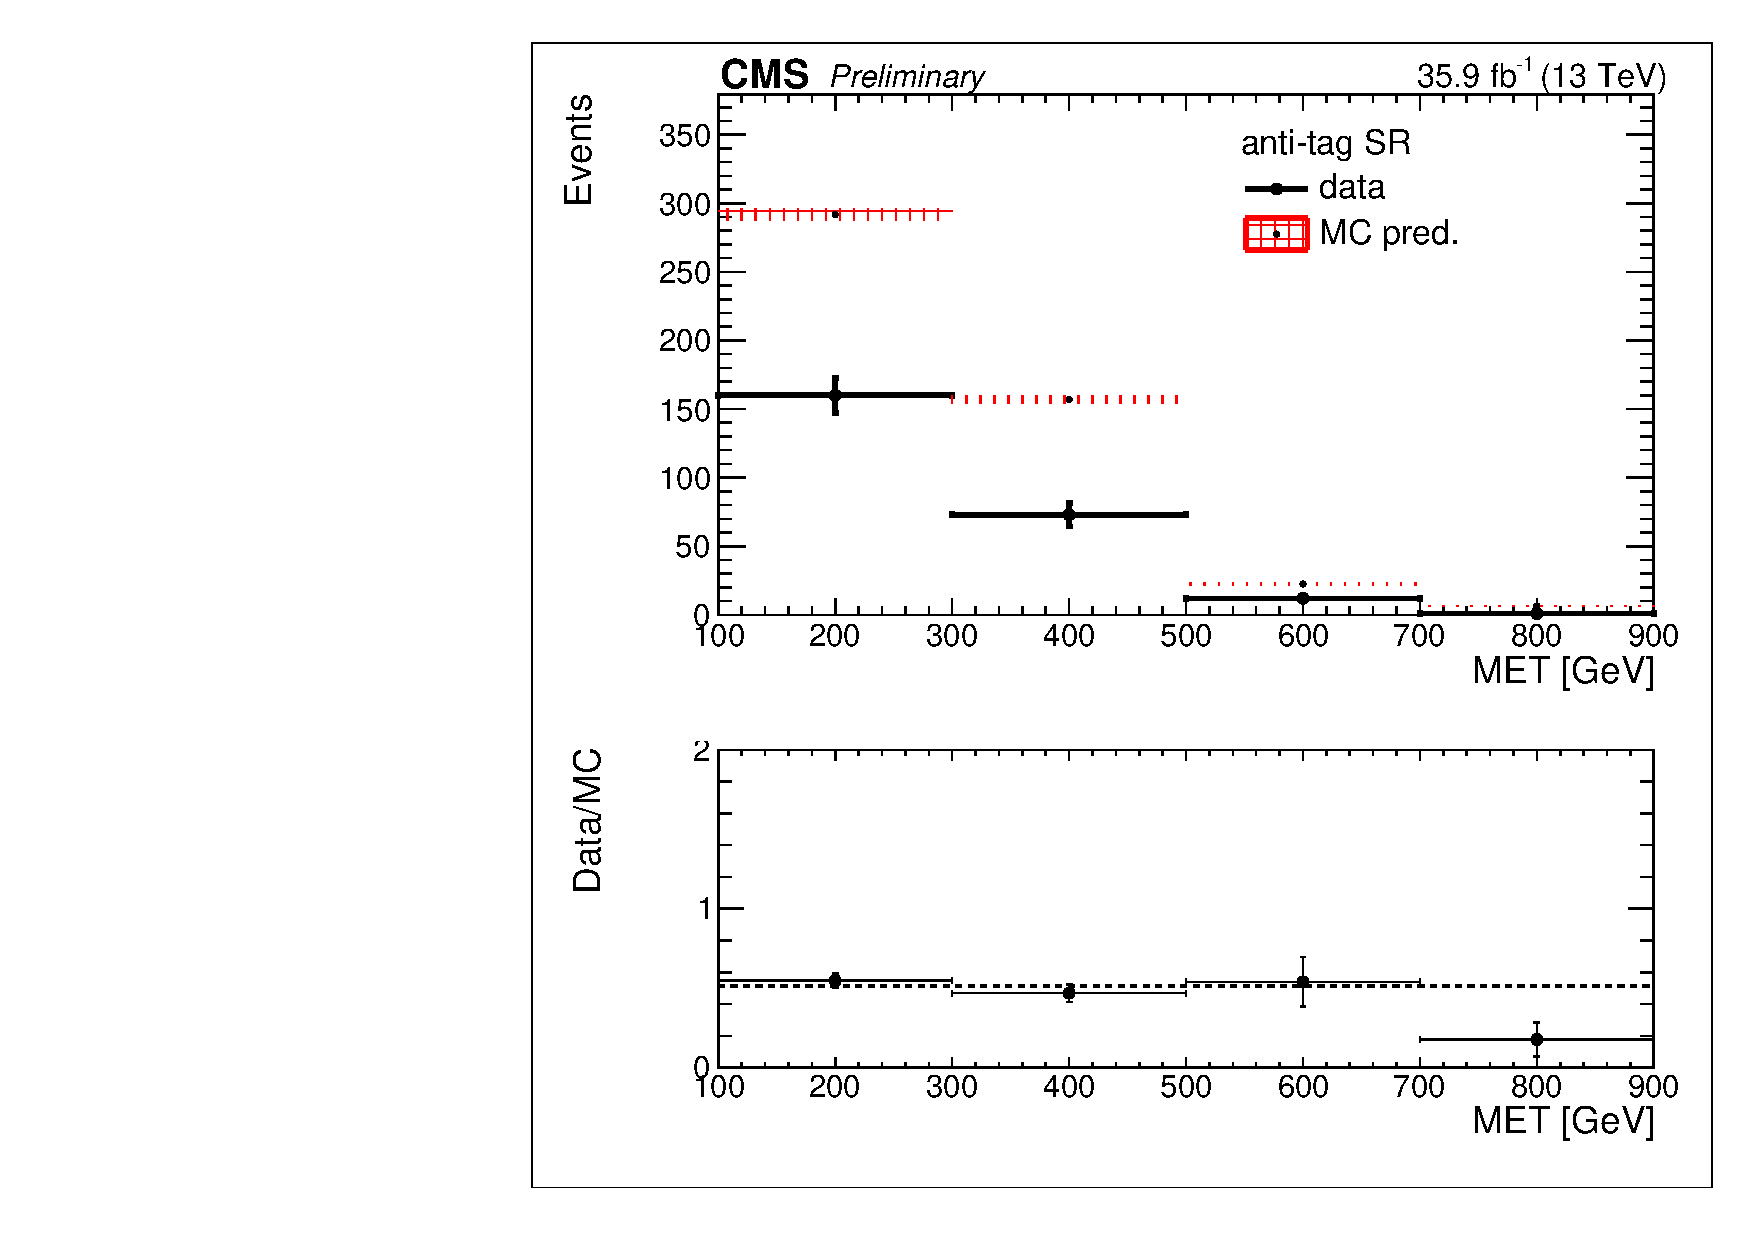
\includegraphics[trim={5px 5px 5px 5px},clip,width=0.425\linewidth]{figs/ABCDscaleFactors_MET_antitagSR_lowDeltaPhi_singleLep.pdf}\\
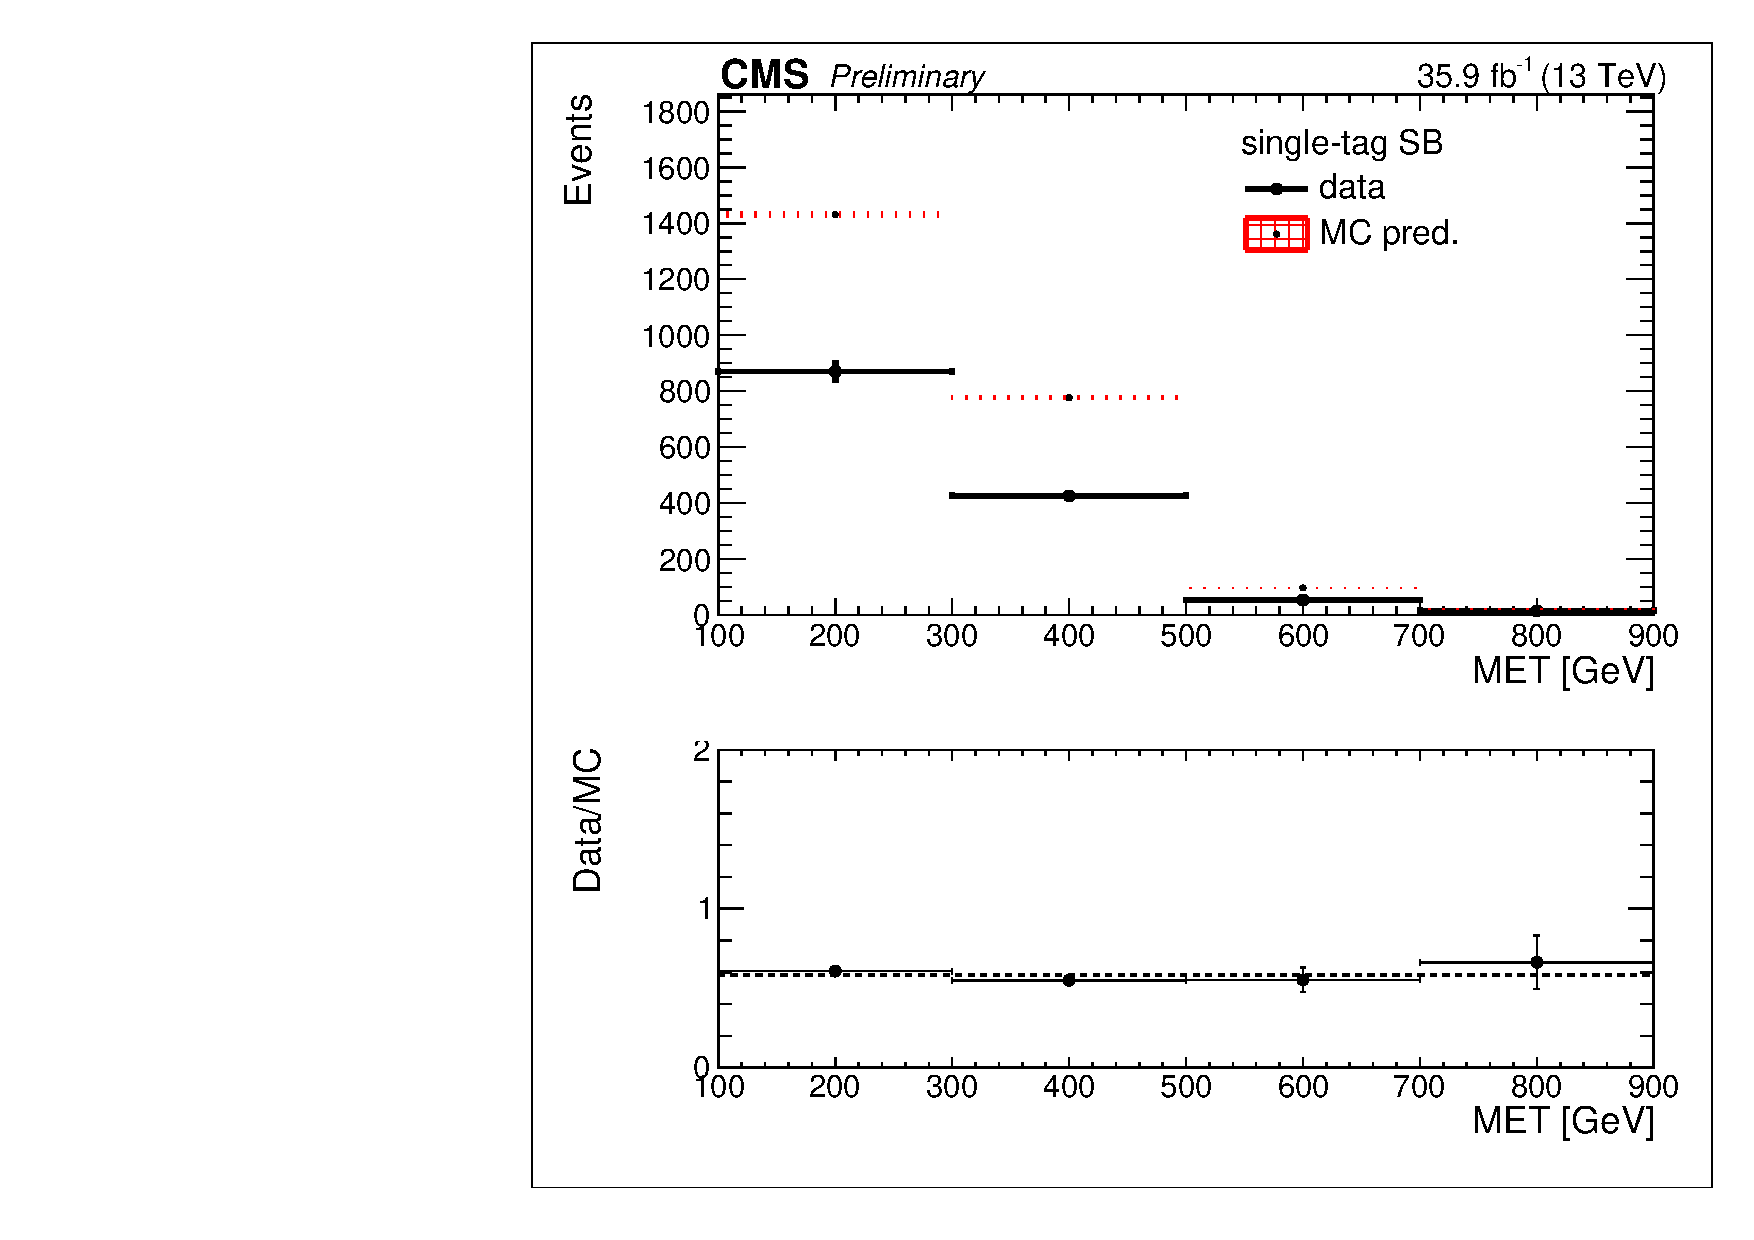
\includegraphics[trim={5px 5px 5px 5px},clip,width=0.425\linewidth]{figs/ABCDscaleFactors_MET_tagSB_lowDeltaPhi_singleLep.pdf}
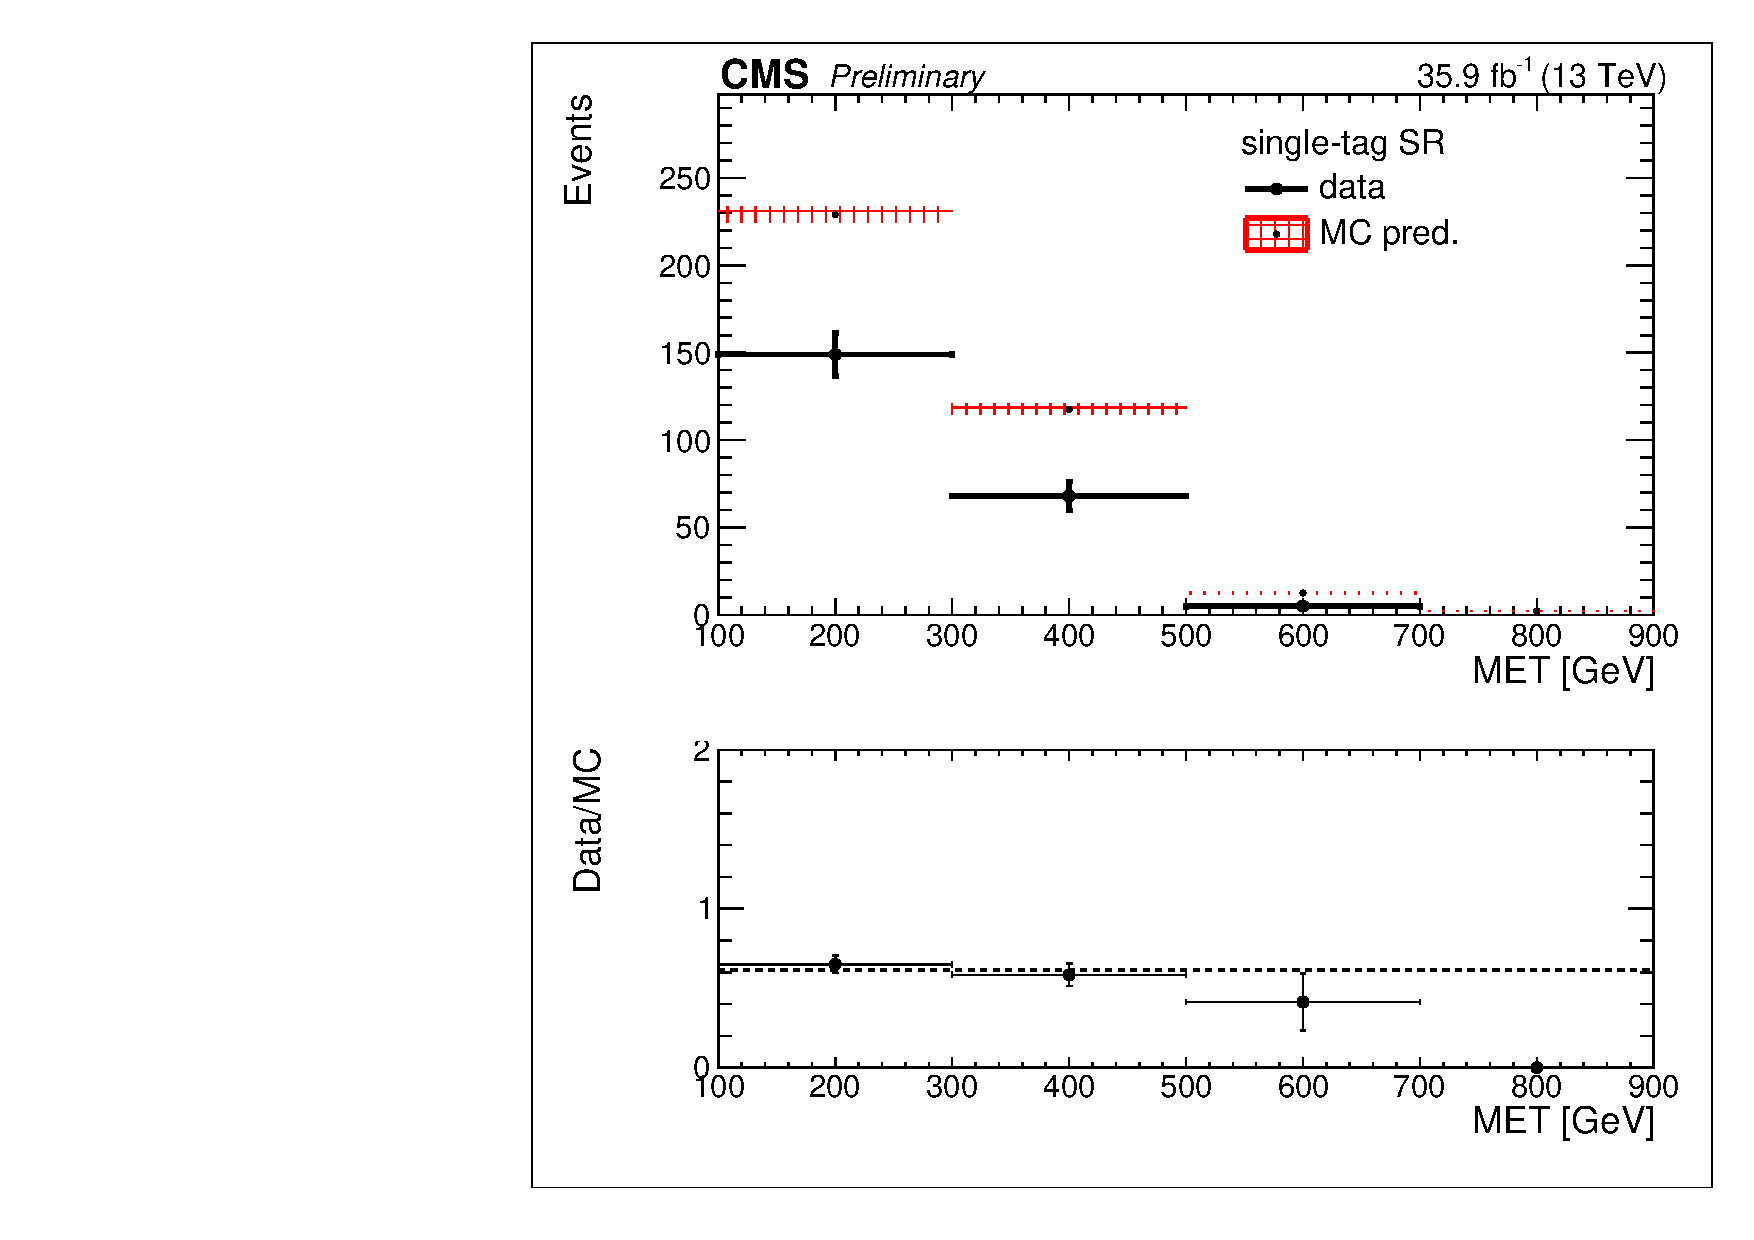
\includegraphics[trim={5px 5px 5px 5px},clip,width=0.425\linewidth]{figs/ABCDscaleFactors_MET_tagSR_lowDeltaPhi_singleLep.pdf}\\
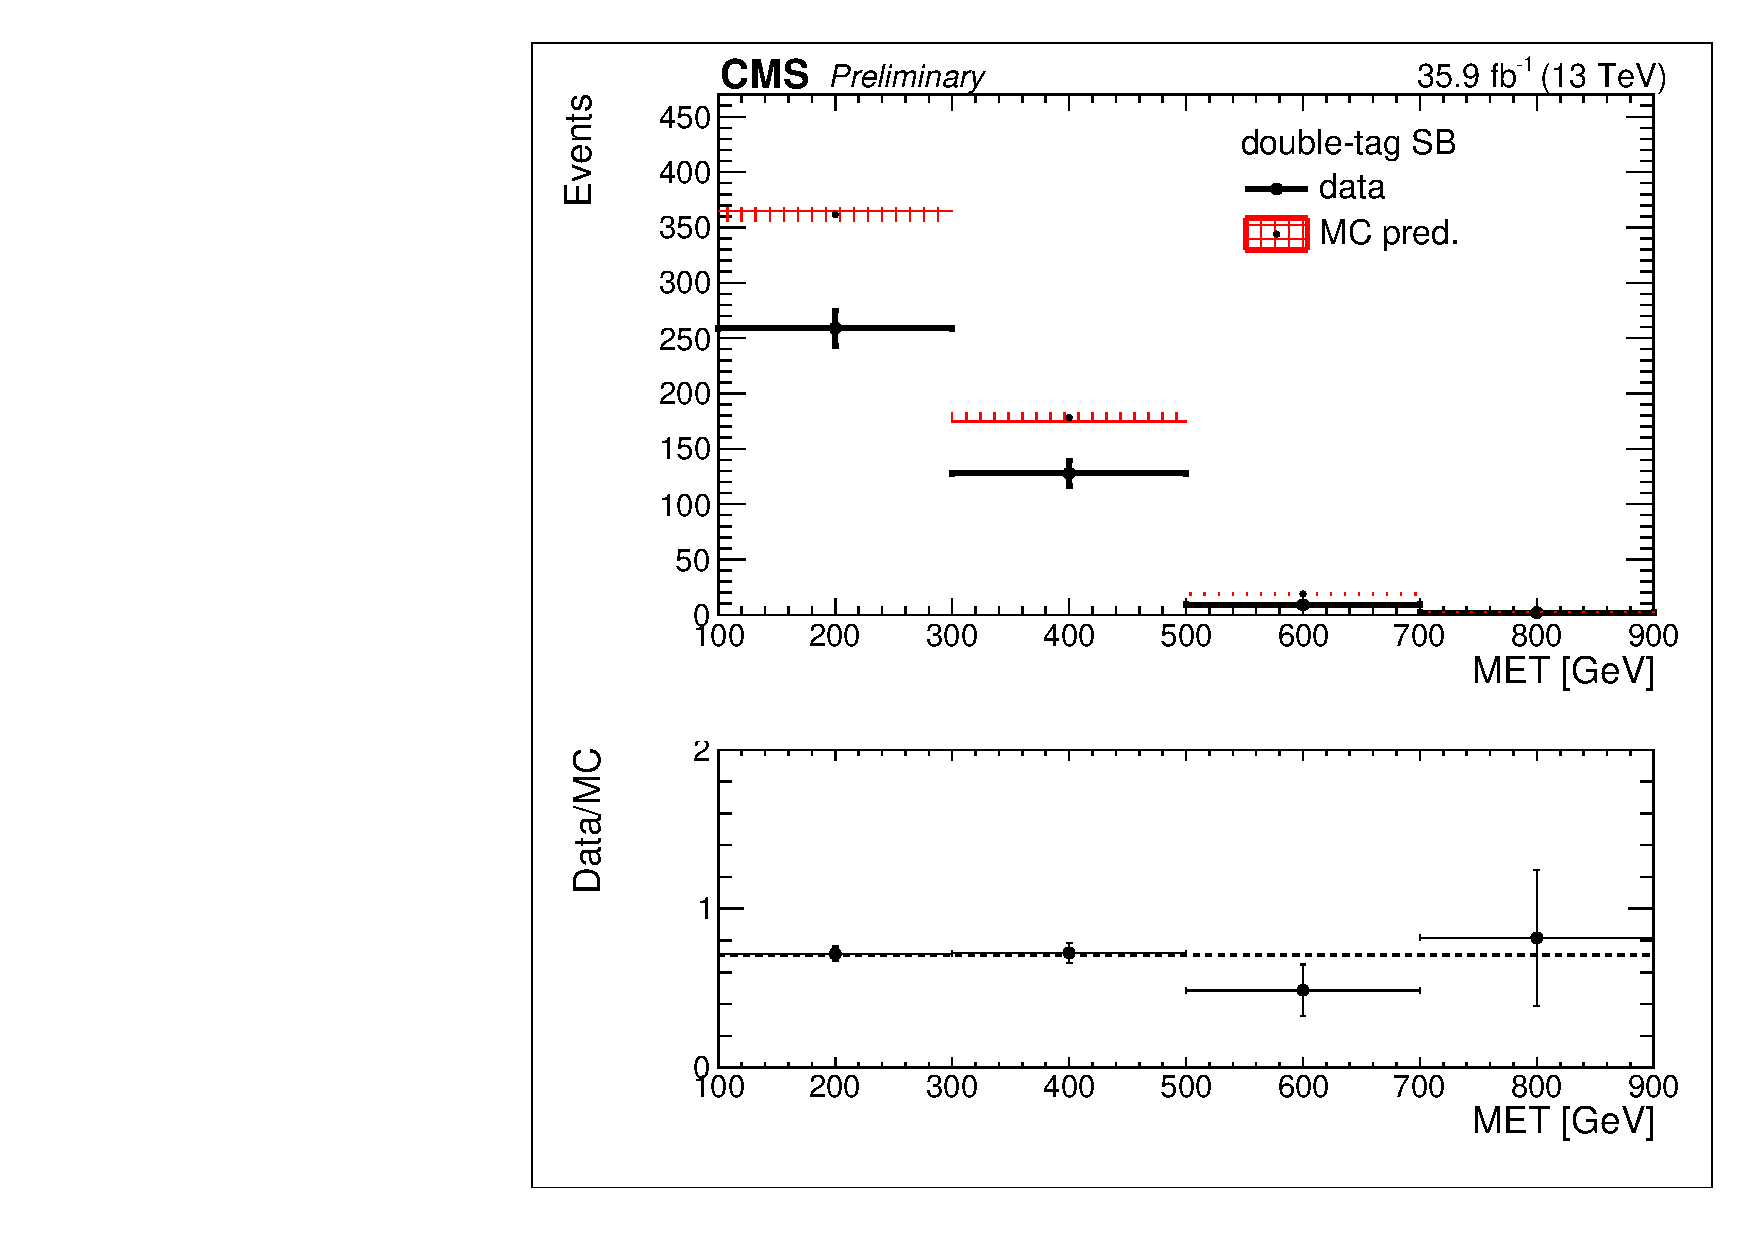
\includegraphics[trim={5px 5px 5px 5px},clip,width=0.425\linewidth]{figs/ABCDscaleFactors_MET_double-tagSB_lowDeltaPhi_singleLep.pdf}
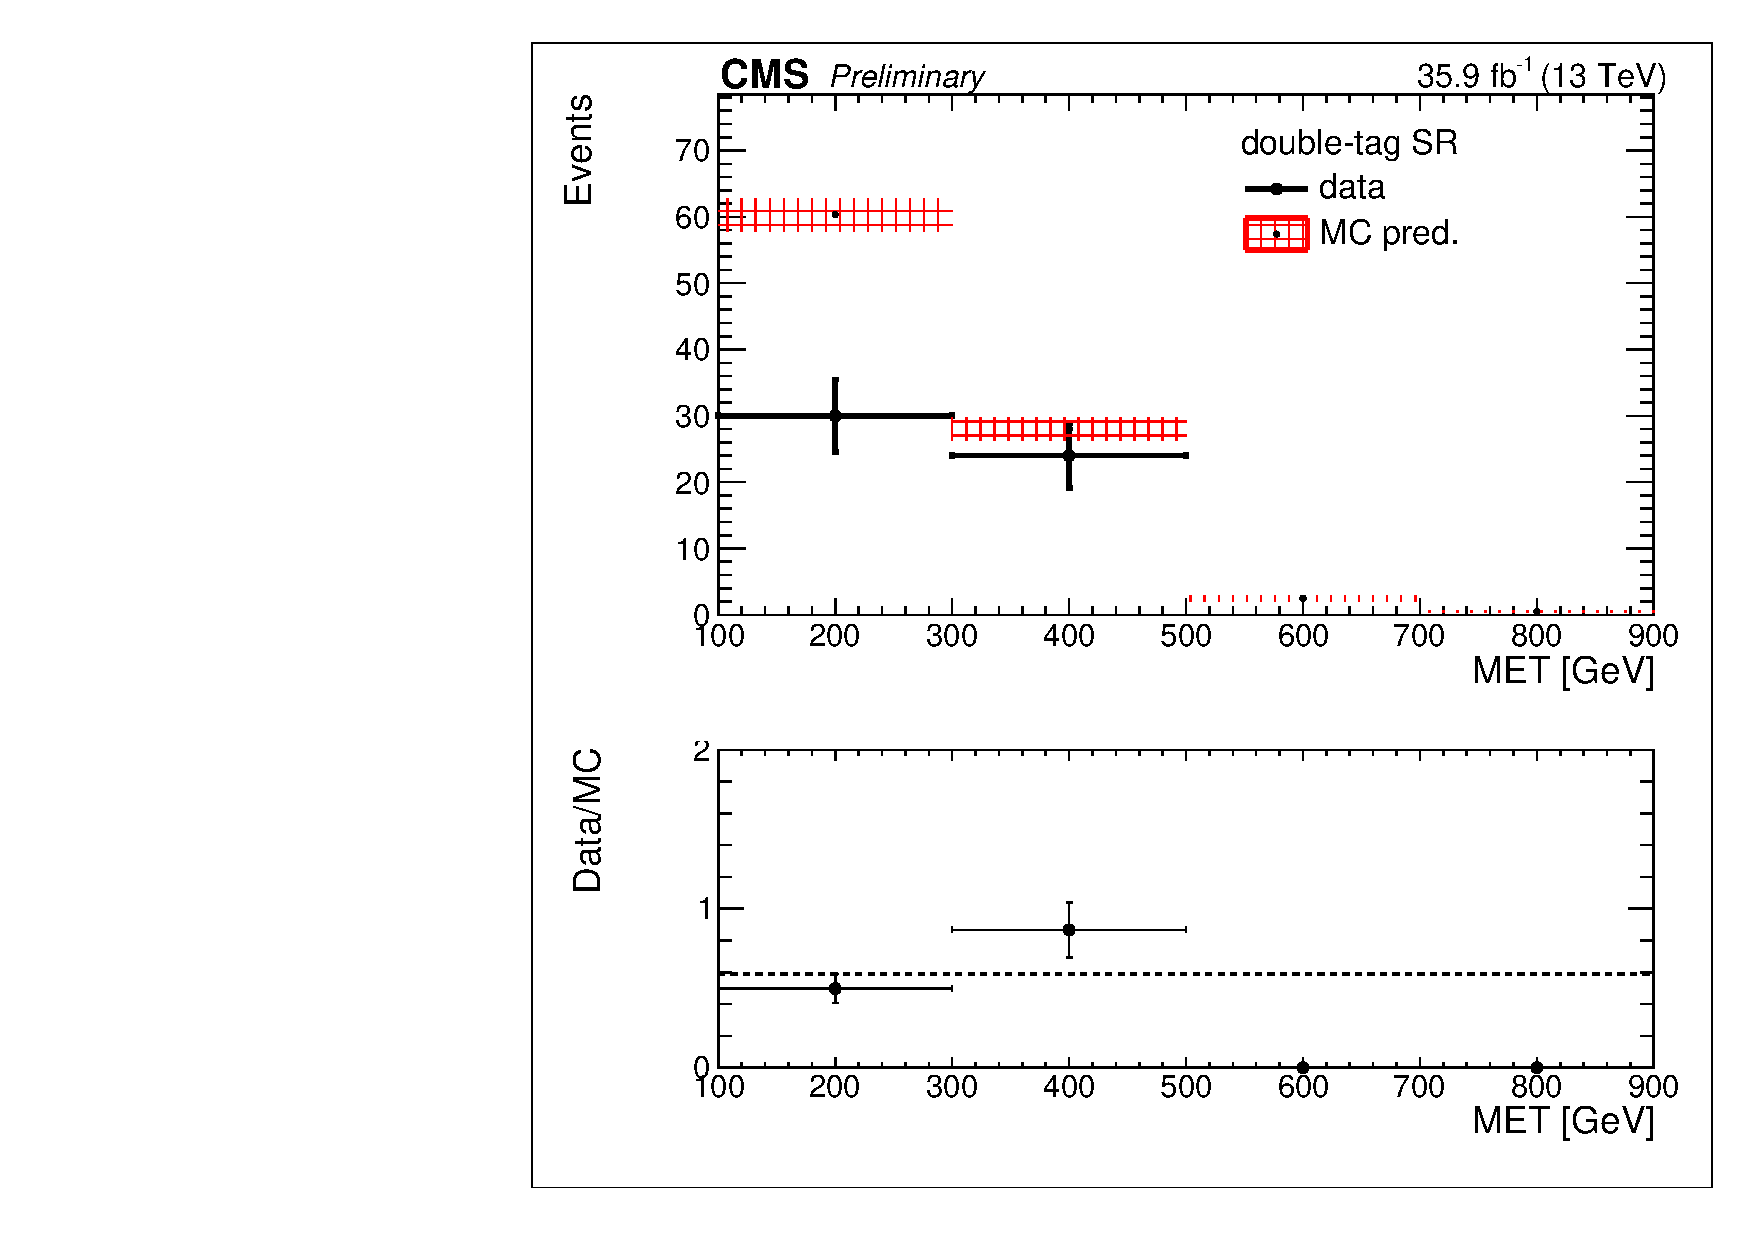
\includegraphics[trim={5px 5px 5px 5px},clip,width=0.425\linewidth]{figs/ABCDscaleFactors_MET_double-tagSR_lowDeltaPhi_singleLep.pdf}\\
\caption
[Signal and sideband yields in the single lepton control region.]
{Signal and sideband yields in the single lepton control region. The hashed red band denotes the prediction from simulation; the solid black points denote the observed yields in data. The Data/MC ratio in the lower panel of each plot represents the scale factor for that bin. The low-$\Delta\phi$ requirement has been removed to improve statistics.}
\label{fig:closuresinglelep}
\end{figure}

\begin{figure}[hbp!]
 \centering
 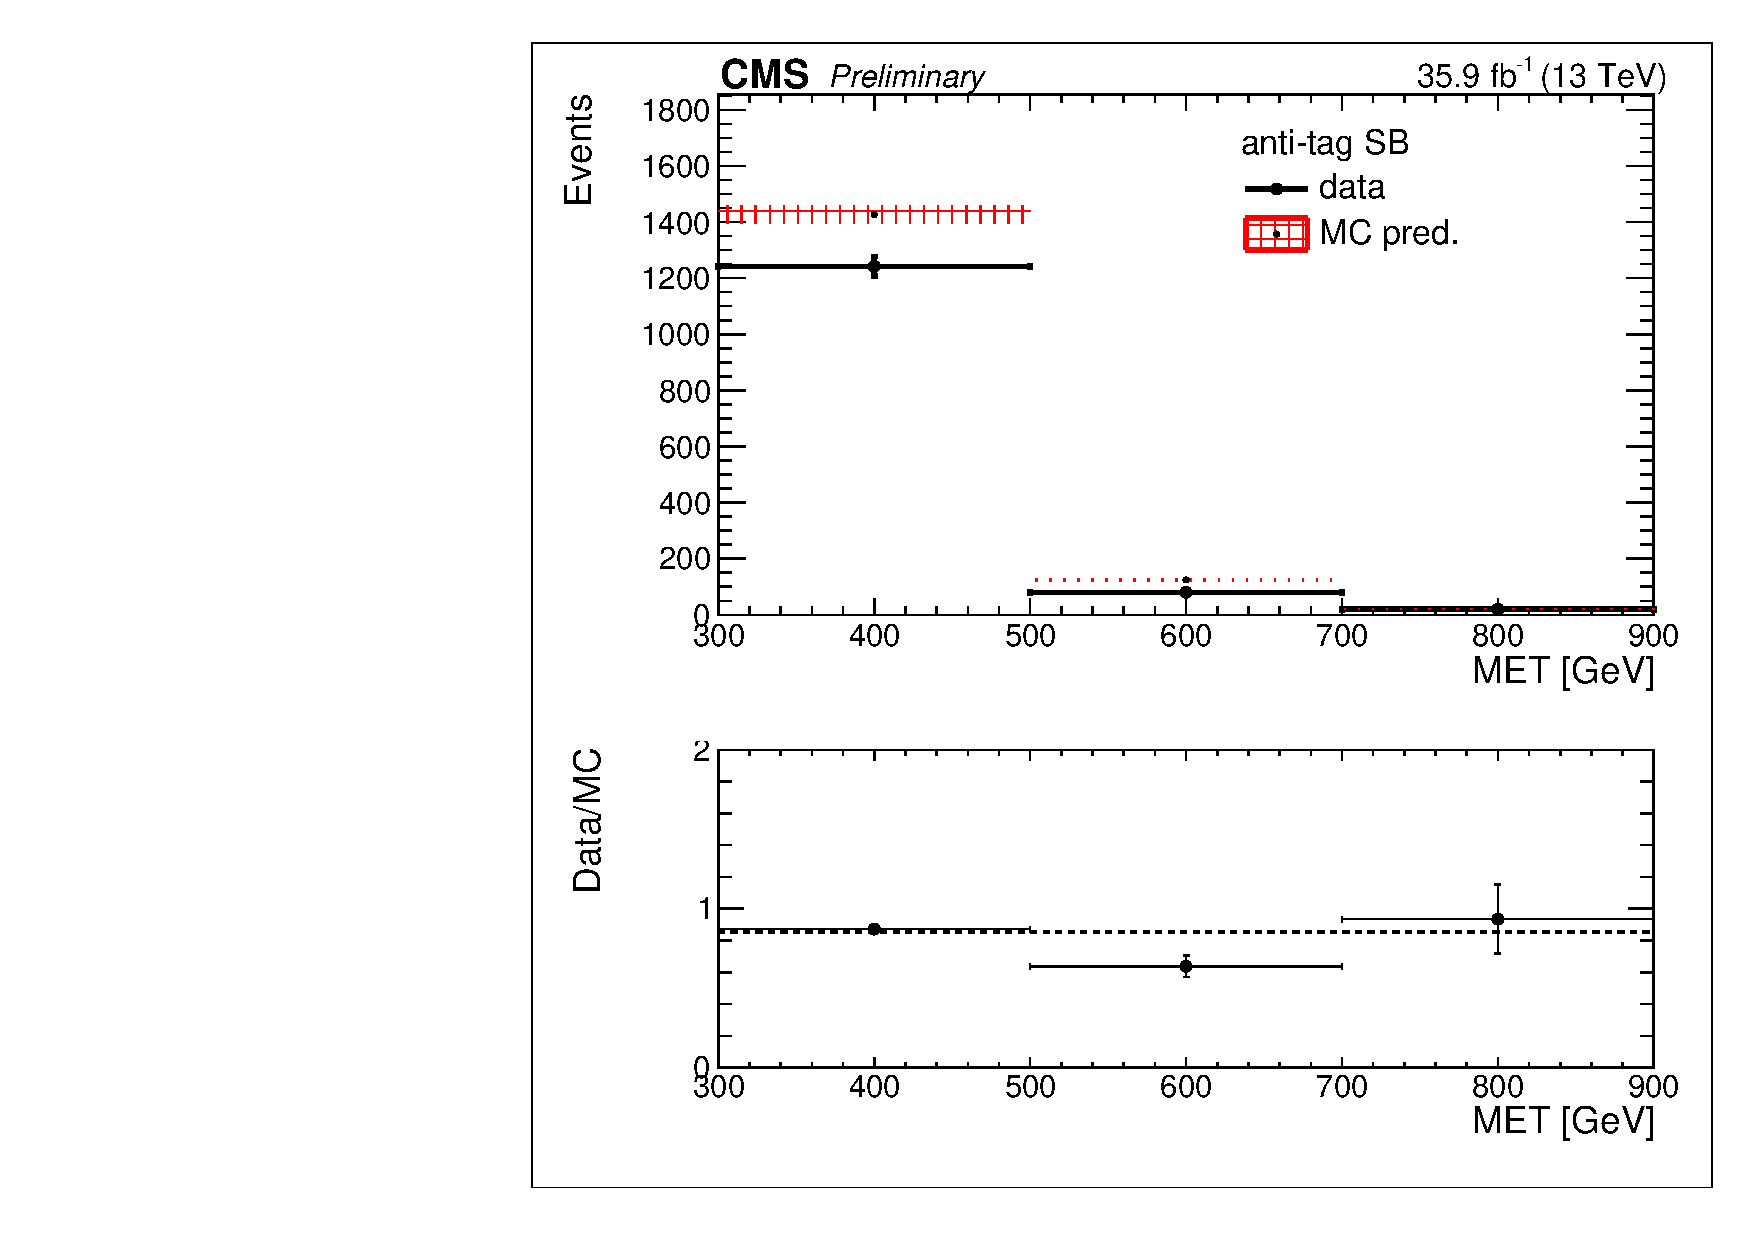
\includegraphics[trim={5px 5px 5px 5px},clip,width=0.425\linewidth]{figs/ABCDscaleFactors_MET_antitagSB_lowDphi.pdf}
 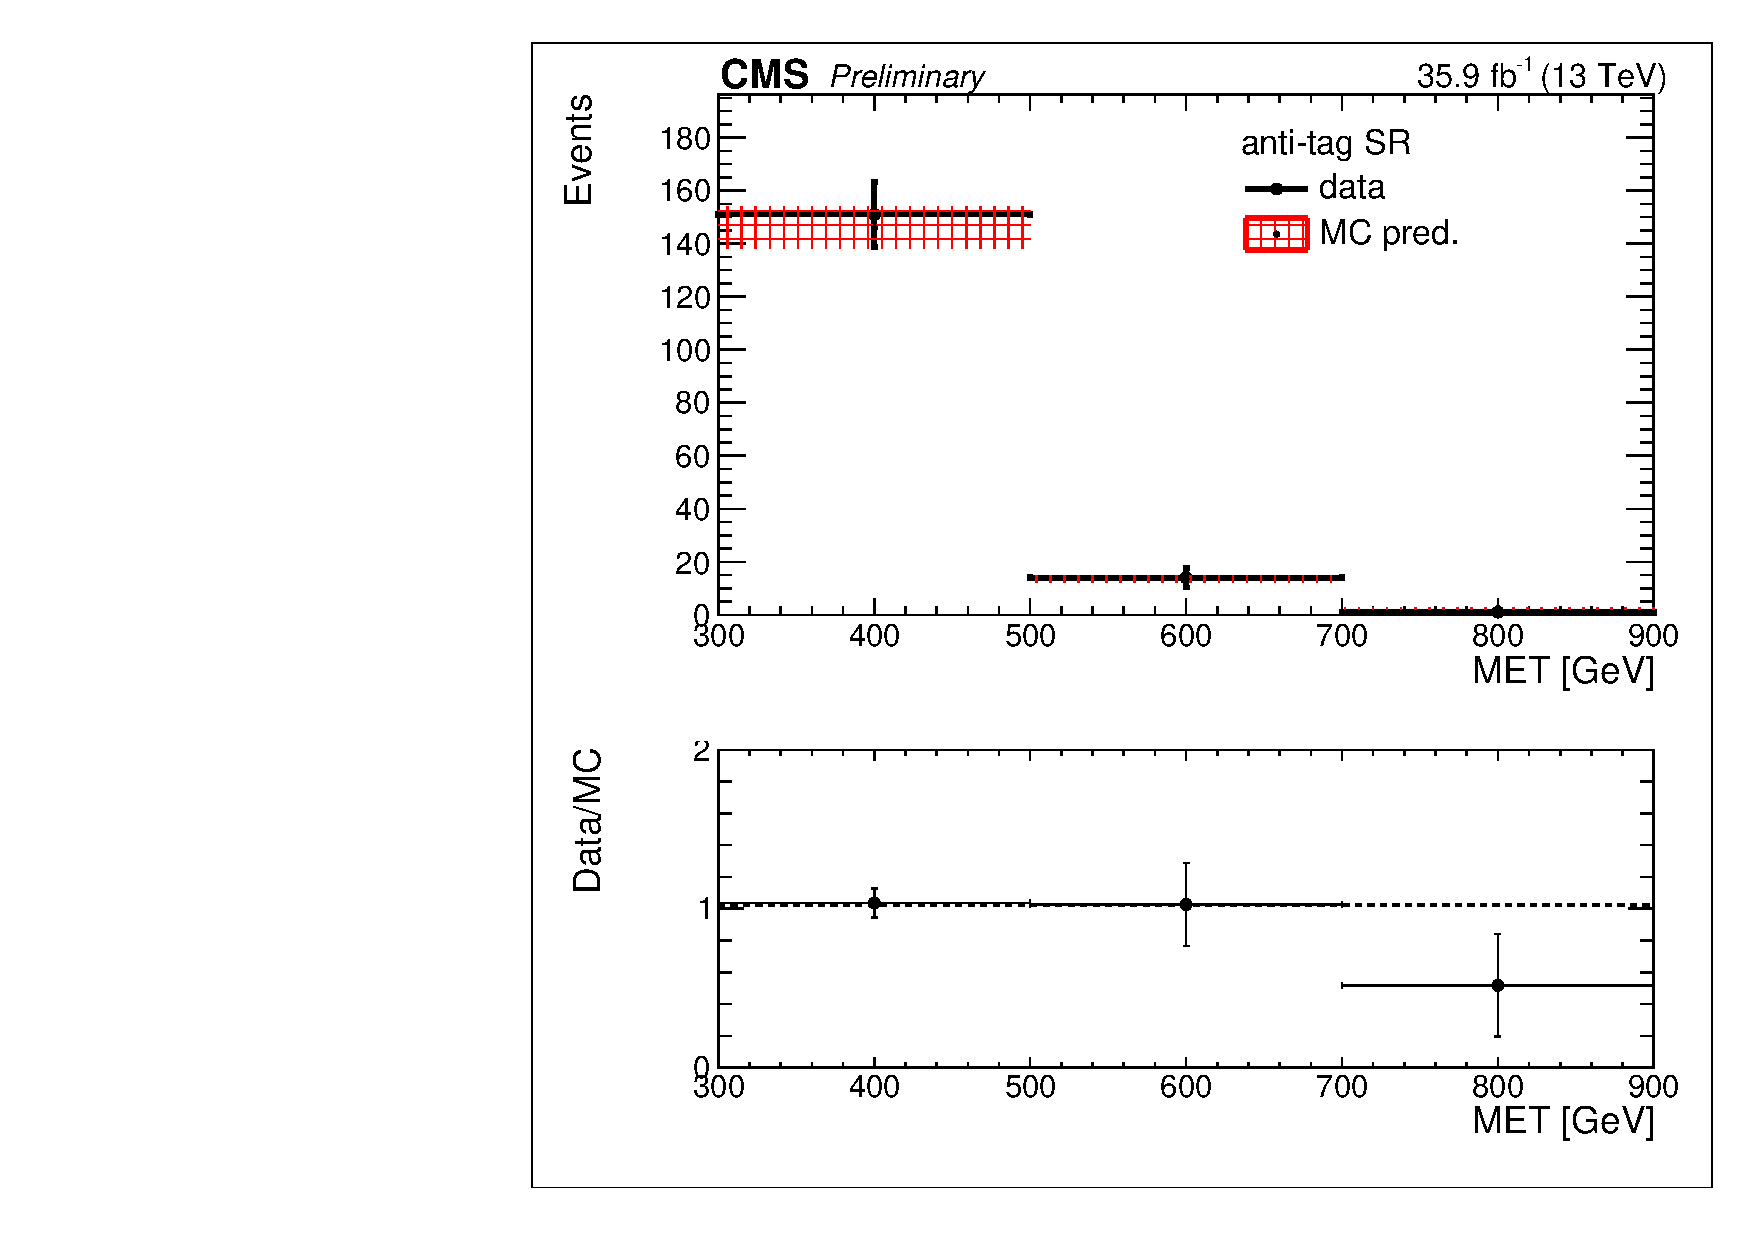
\includegraphics[trim={5px 5px 5px 5px},clip,width=0.425\linewidth]{figs/ABCDscaleFactors_MET_antitagSR_lowDphi.pdf}\\
 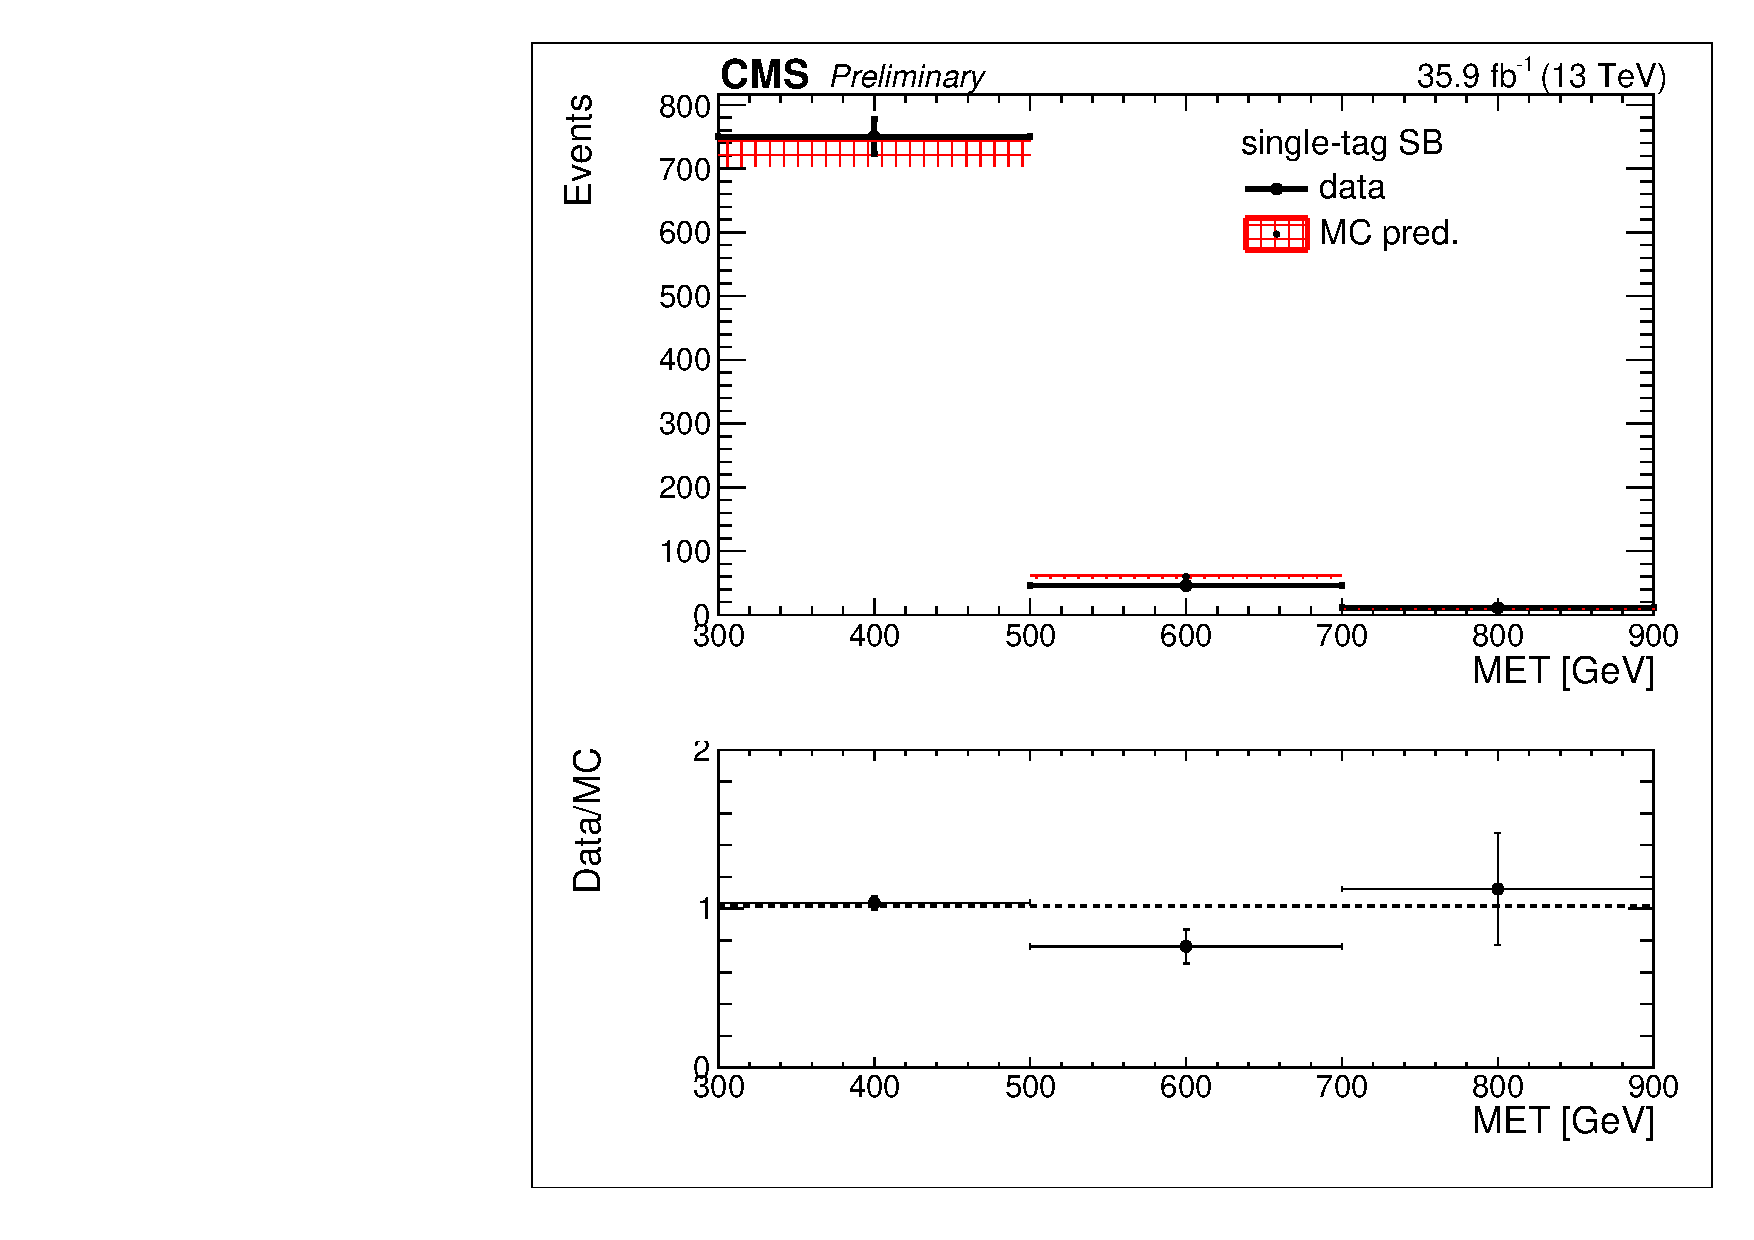
\includegraphics[trim={5px 5px 5px 5px},clip,width=0.425\linewidth]{figs/ABCDscaleFactors_MET_single-tagSB_lowDphi.pdf}
 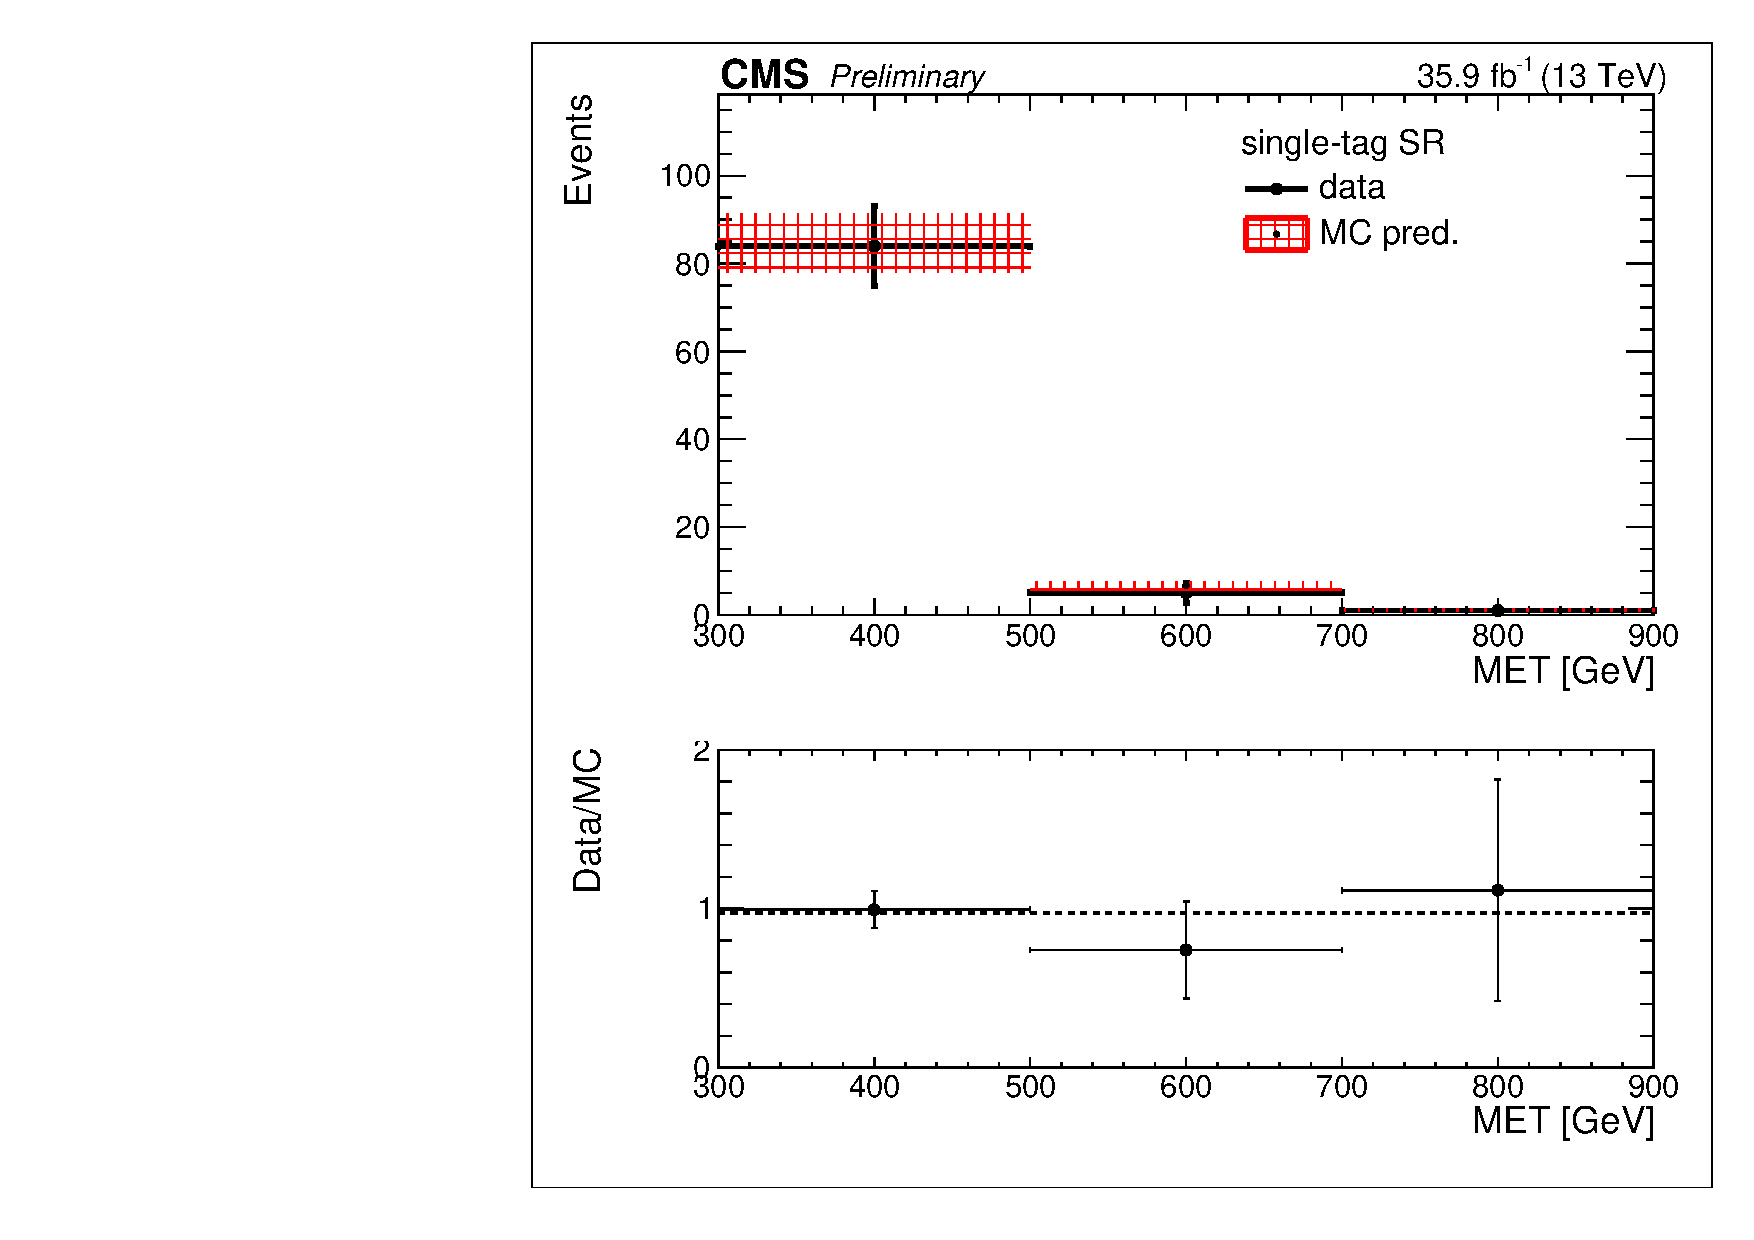
\includegraphics[trim={5px 5px 5px 5px},clip,width=0.425\linewidth]{figs/ABCDscaleFactors_MET_single-tagSR_lowDphi.pdf}\\
 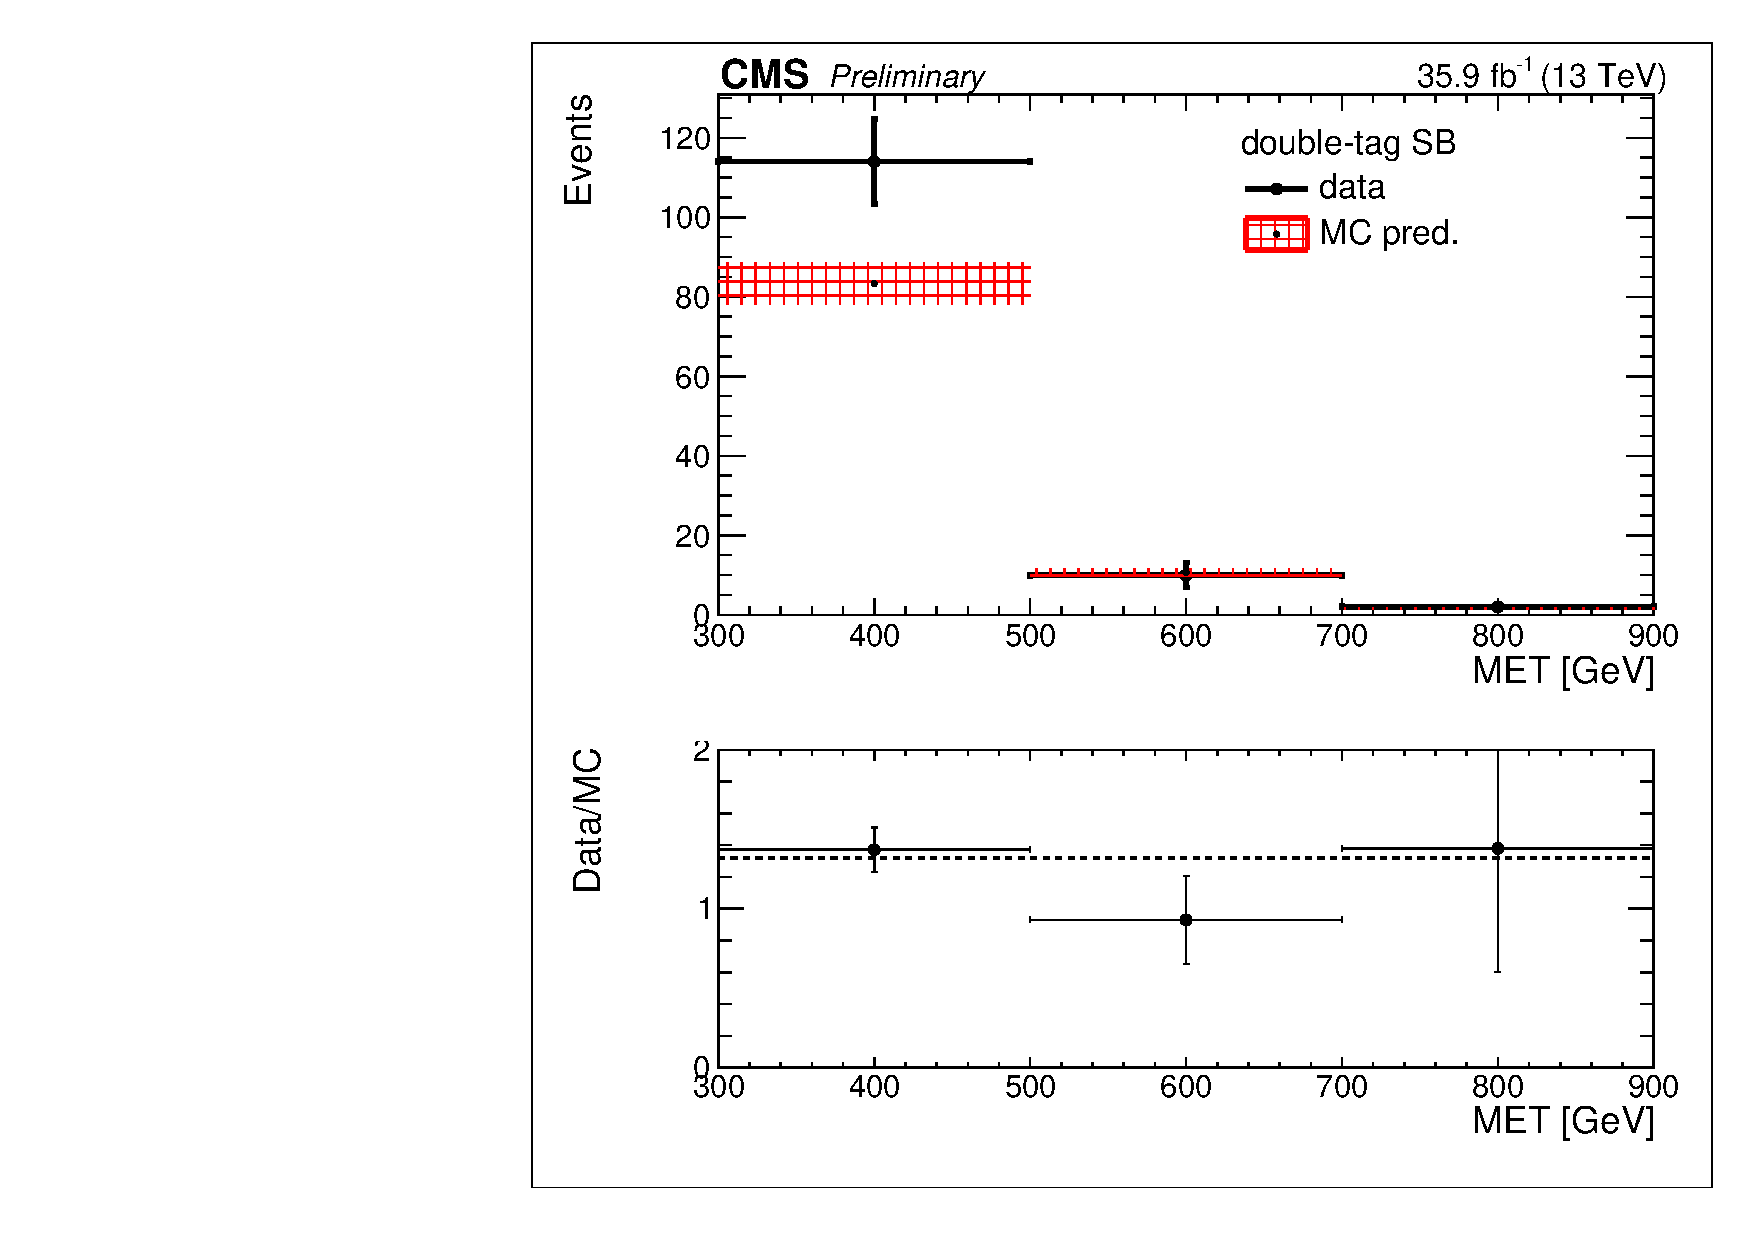
\includegraphics[trim={5px 5px 5px 5px},clip,width=0.425\linewidth]{figs/ABCDscaleFactors_MET_double-tagSB_lowDphi.pdf}
 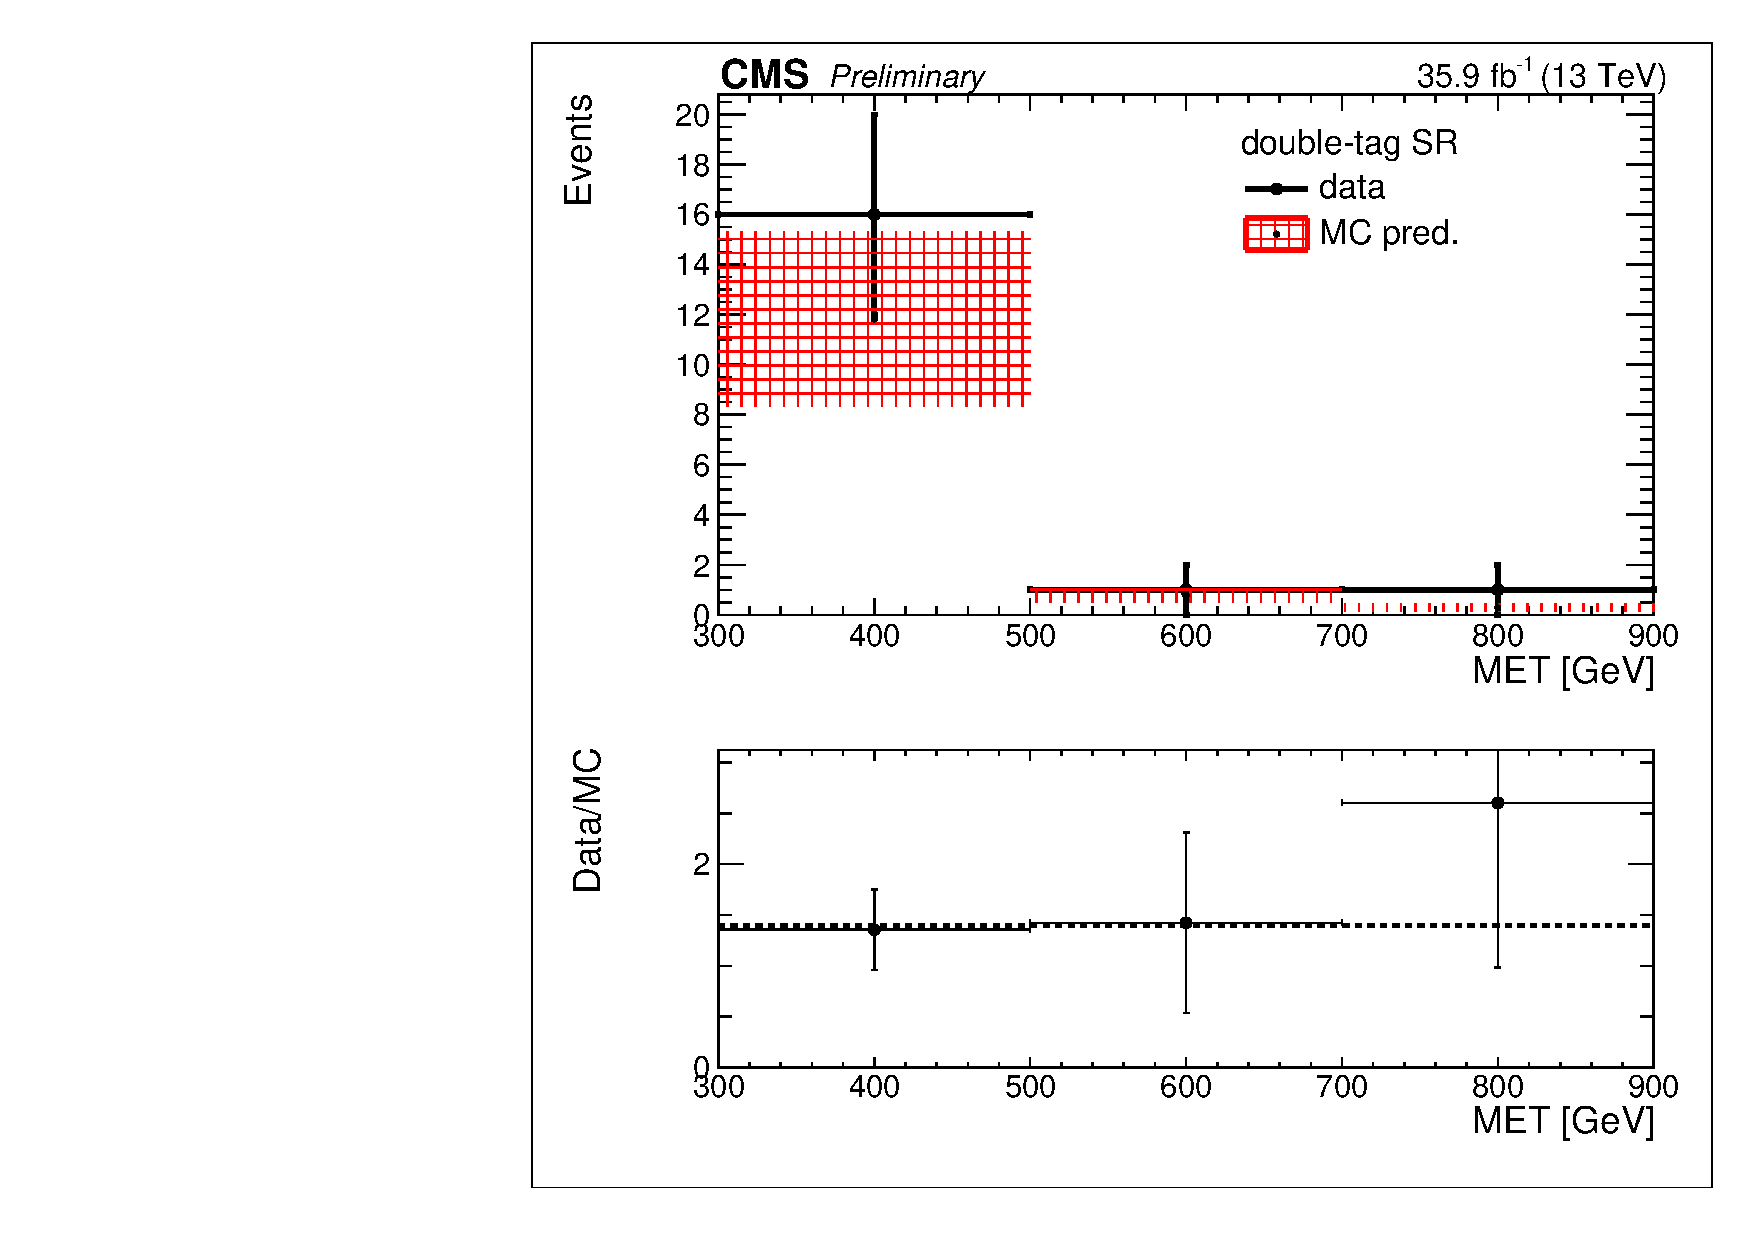
\includegraphics[trim={5px 5px 5px 5px},clip,width=0.425\linewidth]{figs/ABCDscaleFactors_MET_double-tagSR_lowDphi.pdf}\\
 \caption
 [Signal and sideband yields in the the low-$\Delta\phi$ control region.]
 {Signal and sideband yields in the the low-$\Delta\phi$ control region.The hashed red band denotes the prediction from simulation; the solid black points denote the observed yields in data. The Data/MC ratio in the lower panel of each plot represents the scale factor for that bin. }
\label{fig:closurelowdphi}
\end{figure}

\begin{table}[hbp!]
\centering
\caption{Summary of the control region scale-factors integrated over \ptmiss.}
\label{tab:ScaleFactorVR}
\begin{tabular}{c|c|c|c|c|c}
\hline \hline
\multicolumn{6}{c}{Low $\Delta\phi$}\\
\hline \hline
$A^{1H}_{SF}$ & $A^{2H}_{SF}$ & $C_{SF}$ & $B^{1}_{SF}$ & $B^{2}_{SF}$ & $D_{SF}$  \\ \hline
   $1.1 \pm 0.33$ &$0.85 \pm 0.12$&  $0.93 \pm 0.1$ & $0.88 \pm 0.04$ & $1.2 \pm 0.16$  & $0.71 \pm 0.027$ \\ \hline
\hline \hline
\multicolumn{6}{c}{Single Lepton}\\
\hline \hline
$A^{1H}_{SF}$ & $A^{2H}_{SF}$ & $C_{SF}$ & $B^{1}_{SF}$ & $B^{2}_{SF}$ & $D_{SF}$  \\ \hline
   %$0.63 \pm 0.069$ & $0.64 \pm 0.15$  & \MET dependent &   $0.65 \pm 0.1$ & $0.71 \pm 0.059$  & \MET dependent\\ \hline
   %$0.64 \pm 0.033$ & $0.68 \pm 0.068$  & \MET dependent &   $0.63 \pm 0.011$ & $0.72 \pm 0.023$  & \MET dependent\\ \hline
   $0.61\pm 0.04$ & $0.59\pm0.08$ & \ptmiss dependent &  $0.59\pm 0.016$ & $0.71\pm 0.04$  & \ptmiss dependent\\ \hline
\hline \hline
\multicolumn{6}{c}{Photon}\\
\hline \hline
$A^{1H}_{SF}$ & $A^{2H}_{SF}$ & $C_{SF}$ & $B^{1}_{SF}$ & $B^{2}_{SF}$ & $D_{SF}$ \\ \hline
   $0.61 \pm 0.088$ & $0.75 \pm 0.29$ & $0.5 \pm 0.07$ & $0.98 \pm 0.094$ & $2.58 \pm 0.63$ & $0.71 \pm 0.035$\\ \hline
\end{tabular}
\end{table}

\begin{table}[hbp!]
\caption{Single lepton control region scale-factors in the anti-tag sideband region.}
\label{tab:ScaleFactorMET}
\centering
\begin{tabular}{|c|c|c|}
\hline\hline
\multicolumn{3}{c}{Single Lepton $C_{SF}$}\\
\hline
\ptmiss [300, 500] & [500, 700] & [700, $\infty$]\\
$0.47\pm0.05$ & $0.54\pm0.15$ & $0.18\pm 0.1$ \\  \hline\hline
\multicolumn{3}{c}{Single Lepton $D_{SF}$}\\
\hline
$0.49\pm0.02$ & $0.40\pm0.05$ & $0.35\pm 0.08$ \\  
\hline \hline
\end{tabular}
\end{table}

The scale factors are then applied to the MC samples to give yields which better reflect data. The \ptmiss distributions for the signal regions and expectations from the ABCD background prediction are seen in Figure~\ref{fig:mcclosuresf} (the data-corrected version of Figure~\ref{fig:mcclosure}). The improved value of $\kappa$ is seen in the lower panel of each plot. The modified values of the MC yields in the signal region (seen in the calculation of $\kappa$) are seen in Tables~\ref{tab:MCCorrSignal} ~and~\ref{tab:MCCorrControl}. Since most of the scale factors are less than one the background decreases in Figure~\ref{fig:mcclosure} relative to Figure~\ref{fig:mcclosuresf} but still preserves the normalization so that $\kappa$ is statistically compatible with unity. A distribution of $\kappa$ is derived by throwing gaussian toys for each of the scale factors, the final results being summarized in Table~\ref{tab:TotalKappa}.

\begin{table}[hbp!]
\caption{The $\kappa$ factor computed by throwing Gaussian toys for the scale factors.}
\label{tab:TotalKappa}
\centering
\begin{tabular}{c|c|c}
\hline \hline
& 1-Higgs Tag & 2-Higgs Tag\\
\hline \hline
\ptmiss &\multicolumn{2}{c}{$\kappa$} \\  \hline
% $\MET[300,500]$ & $1.03 \pm 0.15$ & $0.82 \pm 0.19$ \\ \hline
% $\MET[500,700]$ & $1.03 \pm 0.22$ & $0.53 \pm 0.17$ \\ \hline
% $\MET>700$ &  $0.83 \pm 0.18$ & $0.61 \pm 0.30$ \\ \hline
[300, 500 GeV] & $0.98 \pm 0.11$ & $0.73 \pm 0.14$ \\ \hline
[500, 700 GeV] & $0.86 \pm 0.16$ & $0.43 \pm 0.12$ \\ \hline
[700, $\infty$ GeV] &  $0.86 \pm 0.17$ & $0.62 \pm 0.30$ \\ \hline
\hline
\end{tabular}
\end{table}

\begin{figure}[hbp!]
\centering
\begin{subfigure}[b]{0.425\textwidth}
\centering
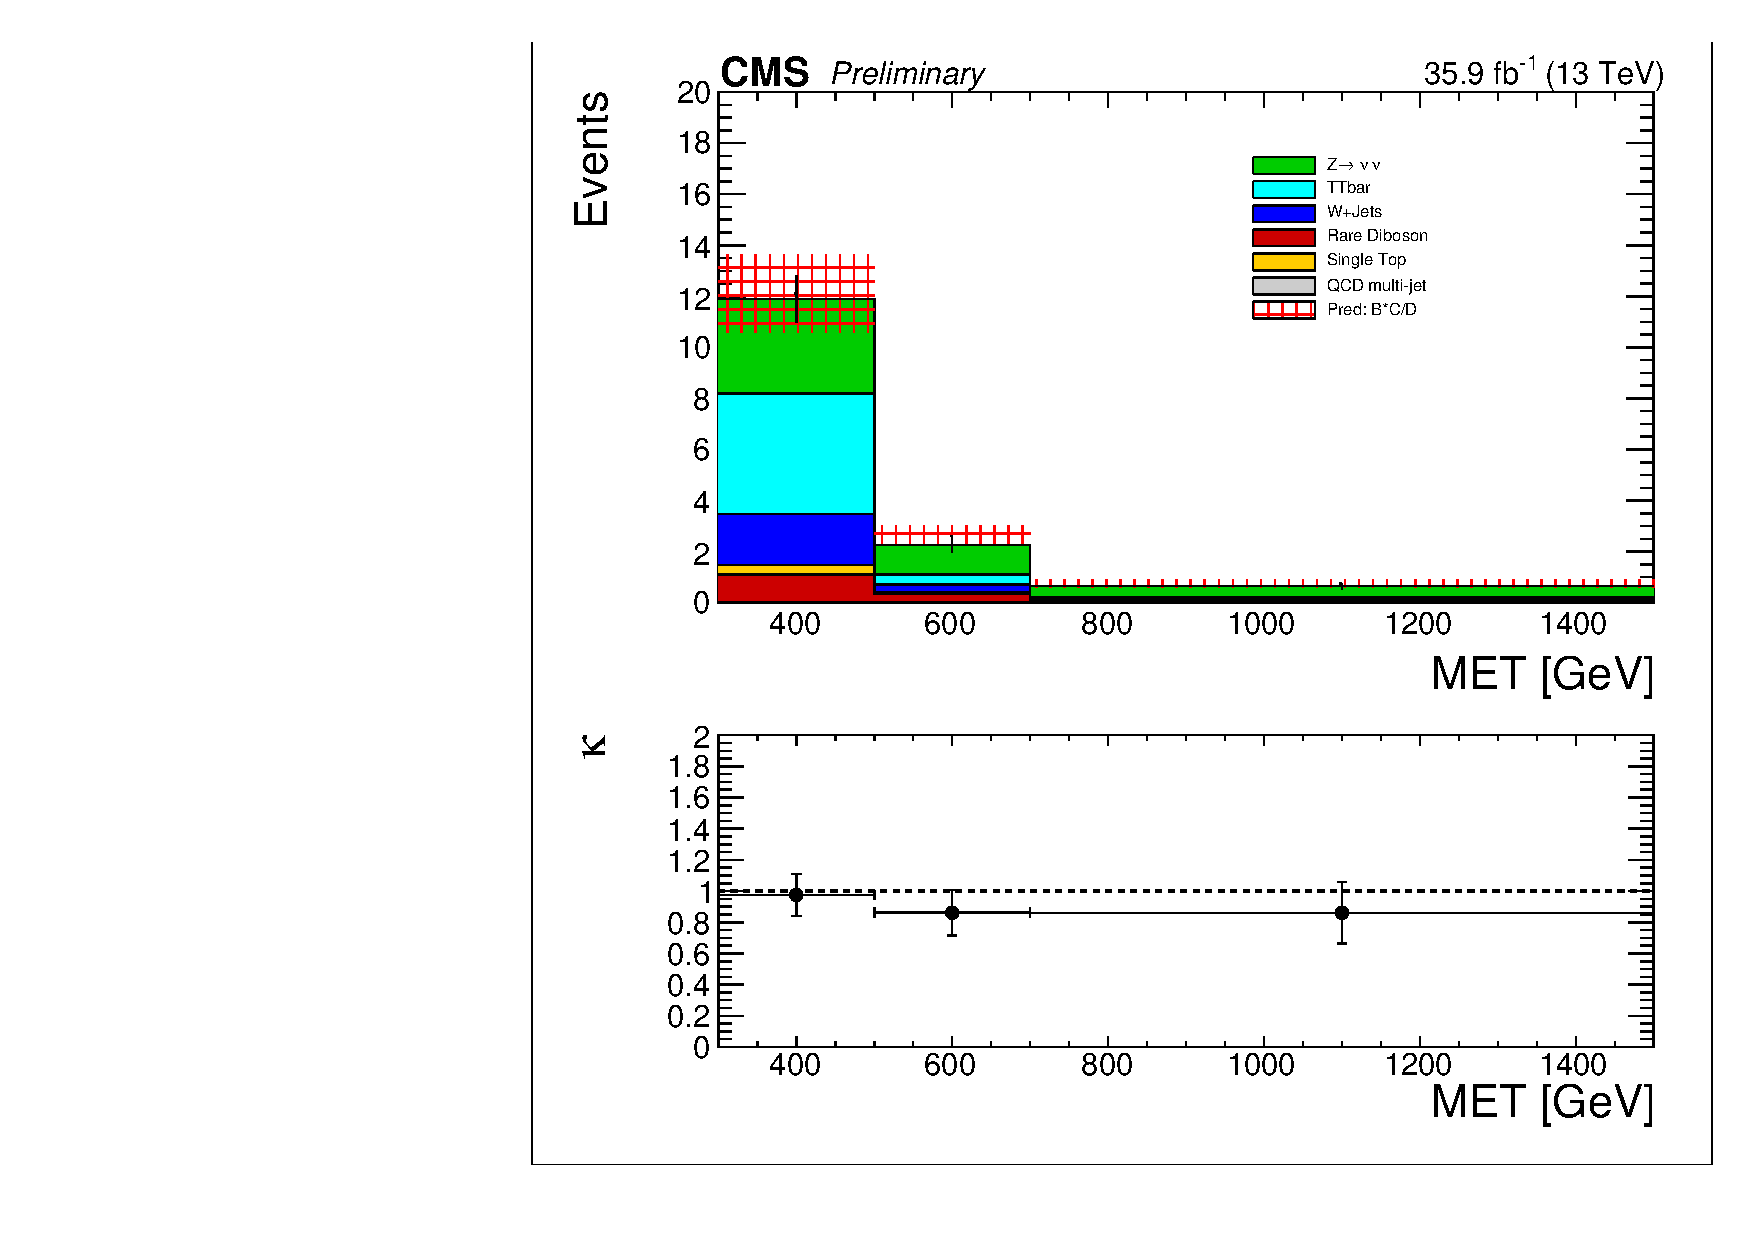
\includegraphics[trim={5px 5px 5px 5px},clip,width=0.95\textwidth]{figs/MCclosureSF_singleHiggsRegionTotal.pdf}
\caption{The single Higgs tag region (A$_{1}$).}
\end{subfigure}
\begin{subfigure}[b]{0.425\textwidth}
\centering
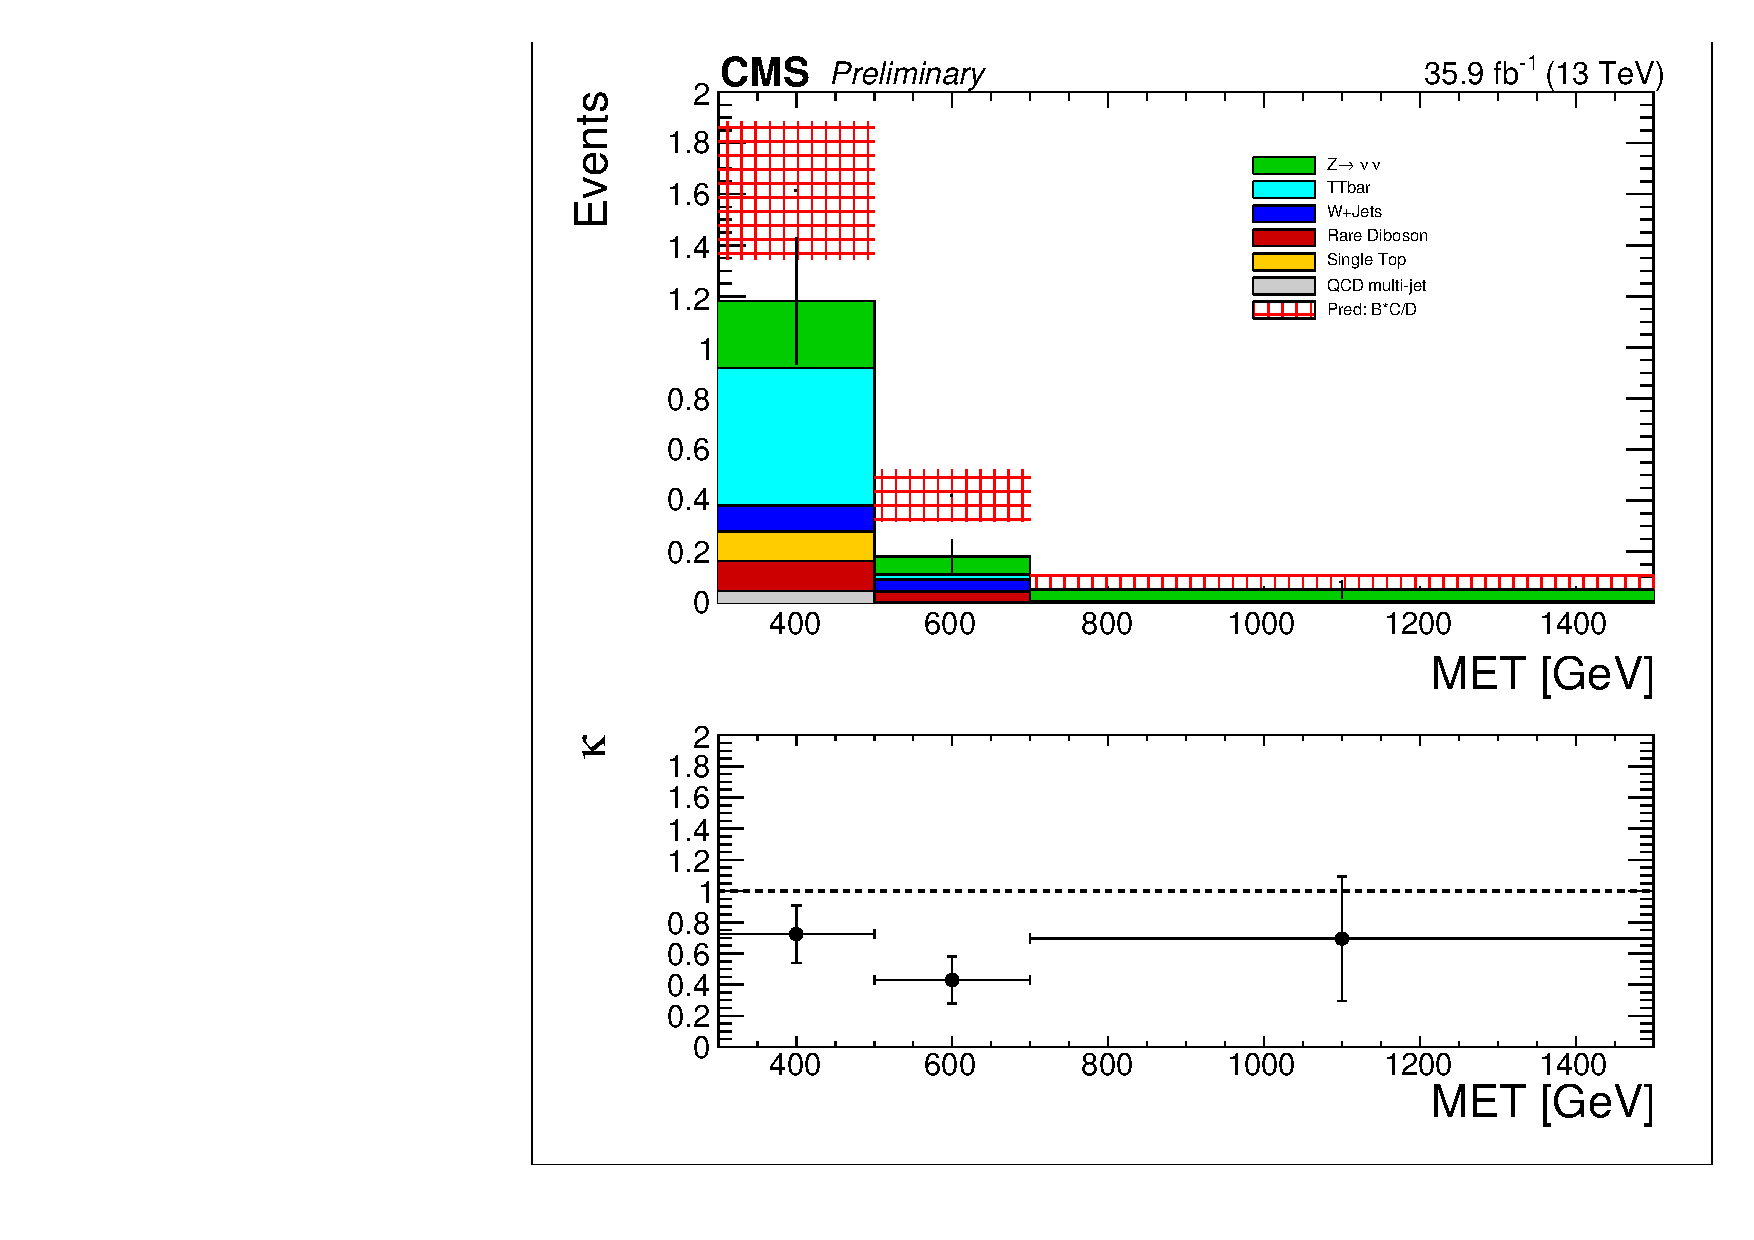
\includegraphics[trim={5px 5px 5px 5px},clip,width=0.95\textwidth]{figs/MCclosureSF_doubleHiggsRegionTotal.pdf} 
\caption{The double Higgs tag region (A$_{2}$).}
\end{subfigure}
\caption{Signal region \ptmiss distributions using scale-factor corrected simulation.}
\label{fig:mcclosuresf}
\end{figure}

\begin{landscape}
\begin{table}
\centering
\caption{Corrected MC yields in the signal regions. $\kappa$ = AD / BC}
\begin{tabular}{c|c|c|c|c|c|c|c|}
\hline \hline
\ptmiss &  Z+Jets  & W+Jets & TTbar & QCD & Rare & Total  & Data \\ \hline \hline
\multicolumn{8}{c}{Region: $A^{1H}$}  \\ \hline \hline
$[300,500]$ GeV & 3.76 $\pm$ 0.54 & 2.05 $\pm$ 0.30 & 4.87 $\pm$ 0.72& 0 $\pm$ 0 & 1.48 $\pm$ 0.40 & 12.17 $\pm$ 1.03 &   15\\ \hline
$[500,700]$ GeV & 1.18 $\pm$ 0.21 & 0.33 $\pm$ 0.08 & 0.40$\pm$ 0.12& 0 $\pm$ 0 & 0.39$\pm$ 0.16 &   2.30 $\pm$ 0.29 & 2
\\ \hline 
$>700$ GeV & 0.43 $\pm$ 0.10 & 0.053$\pm$ 0.025& 0.046 $\pm$ 0.01& 0 $\pm$ 0 & 0.13 $\pm$ 0.053&   0.66$\pm$ 0.12& 1
\\ \hline
\multicolumn{8}{c}{Region: $A^{2H}$}  \\ \hline \hline
$[300,500]$ GeV & 0.26 $\pm$ 0.12 & 0.11 $\pm$ 0.05 & 0.58$\pm$ 0.21& 0.045$\pm$ 0.05 & 0.23$\pm$ 0.12   & 1.24 $\pm$ 0.28 & 1  \\ \hline
$[500,700]$ GeV & 0.07 $\pm$ 0.045 & 0.049 $\pm$ 0.031 & 0.022 $\pm$ 0.0098 & 0 $\pm$ 0 & 0.045 $\pm$ 0.039 &   0.19 $\pm$ 0.068 & 0\\  \hline
$>700$ GeV  & 0.044 $\pm$ 0.032& 0.005$\pm$ 0.005 & 0 $\pm$ 0 & 0 $\pm$ 0 & 0.002 $\pm$ 0.016  & 0.051 $\pm$ 0.036 &  0\\  \hline 
\end{tabular}
\end{table}
\begin{table}
\centering
\caption{Corrected MC yields in the sideband regions. $\kappa$ = AD / BC} 
\label{tab:MCCorrSignal}

\begin{tabular}{c|c|c|c|c|c|c|c|}
\hline \hline
\ptmiss &  Z+Jets  & W+Jets & TTbar & QCD & Rare & Total  & Data \\
\hline \hline
\multicolumn{8}{c}{Region: $C$}  \\ \hline \hline
$[300,500]$ GeV & 17.66 $\pm$ 2.52 & 8.23 $\pm$ 1.44 & 3.87 $\pm$ 0.73 & 0.81 $\pm$ 0.49& 2.78 $\pm$ 1.142   & 33.36 $\pm$ 3.24 & 44 \\ \hline
$[500,700]$ GeV & 5.20$\pm$ 0.77& 0.57 $\pm$ 0.27 & 0.22 $\pm$ 0.11 & 0 $\pm$ 0 & 0.63 $\pm$ 0.16   & 6.63 $\pm$ 0.84 & 12
\\ \hline 
$>700$ GeV & 2.48 $\pm$ 0.39& 0.12 $\pm$ 0.12 & 0.028$\pm$ 0.031 & 0 $\pm$ 0 & 0.14 $\pm$ 0.06   & 2.76 $\pm$ 0.41 & 4
\\ \hline
\multicolumn{8}{c}{Region: $B^{1H}$}  \\ \hline \hline
$[300,500]$ GeV & 42.13 $\pm$ 4.17& 15.61 $\pm$ 10.15 & 30.99 $\pm$ 20.15 & 1.57 $\pm$ 0.54 & 12.16 $\pm$ 1.37   & 102.47 $\pm$ 23.00 & 112  \\ \hline
$[500,700]$ GeV & 12.05 $\pm$ 1.28 & 2.74 $\pm$ 1.79 & 3.04 $\pm$ 2.00 & 0 $\pm$ 0 & 2.55 $\pm$ 0.43   & 20.37 $\pm$ 3.00 & 20\\  \hline
$>700$ GeV  &5.92 $\pm$ 0.69& 0.67 $\pm$ 0.61& 0.49$\pm$ 0.46 & 0 $\pm$ 0 & 1.93 $\pm$ 0.72   & 9.01 $\pm$ 1.25 & 5  \\  \hline  
\multicolumn{8}{c}{Region: $B^{2H}$}  \\ \hline \hline
$[300,500]$ GeV & 5.51 $\pm$ 1.47 & 0.73 $\pm$ 0.44 & 4.46 $\pm$ 2.65 & 0.33 $\pm$ 0.23 & 2.06 $\pm$ 0.32 & 13.09 $\pm$ 3.09 & 13 
\\ \hline
$[500,700]$ GeV & 1.80 $\pm$ 0.56 & 0.17 $\pm$ 0.11 & 0.59 $\pm$ 0.39 & 0 $\pm$ 0 & 0.62 $\pm$ 0.23 & 3.17 $\pm$ 0.73 & 1 \\ \hline
$>700$ GeV  & 0.67 $\pm$ 0.27 & 0.0084 $\pm$ 0.009& 0.035 $\pm$ 0.031& 0 $\pm$ 0 & 0.23 $\pm$ 0.073   & 0.94 $\pm$ 0.28 & 1  \\  \hline  
\multicolumn{8}{c}{Region: $D$}  \\ \hline \hline
$[300,500]$ GeV & 164.82$\pm$ 8.31 & 61.24 $\pm$ 3.70 & 33.20 $\pm$ 2.16 & 8.50 $\pm$ 2.73 & 20.64 $\pm$ 1.78   & 288.41 $\pm$ 9.90 & 273  \\ \hline
$[500,700]$ GeV & 47.37 $\pm$ 2.52 & 6.36 $\pm$ 1.39 & 2.37 $\pm$ 0.55 & 0 $\pm$ 0 & 4.42$\pm$ 1.46 &   60.51 $\pm$ 3.27 & 60\\  \hline
$>700$ GeV  & 26.79 $\pm$ 1.50 & 0.99 $\pm$ 0.53 & 0.16 $\pm$ 0.086 & 0 $\pm$ 0 & 3.48 $\pm$ 1.01  & 31.42 $\pm$ 1.88& 28  \\  \hline  
\end{tabular}
\label{tab:MCCorrControl}
\end{table}
\end{landscape}

\subsection{Sideband Yields \& Predictions}

Observed yields in data and the MC expectation for the 12 sideband bins (e.g. $\mathrm{B}_{1, 2}$, C, D in Figure~\ref{fig:abcd}) are seen in Figure~\ref{fig:UnblindCR}. Table~\ref{tab:tab} lists these observed yields and calculated background prediction for the 6 signal bins.

\begin{figure}[hbp!]
\centering
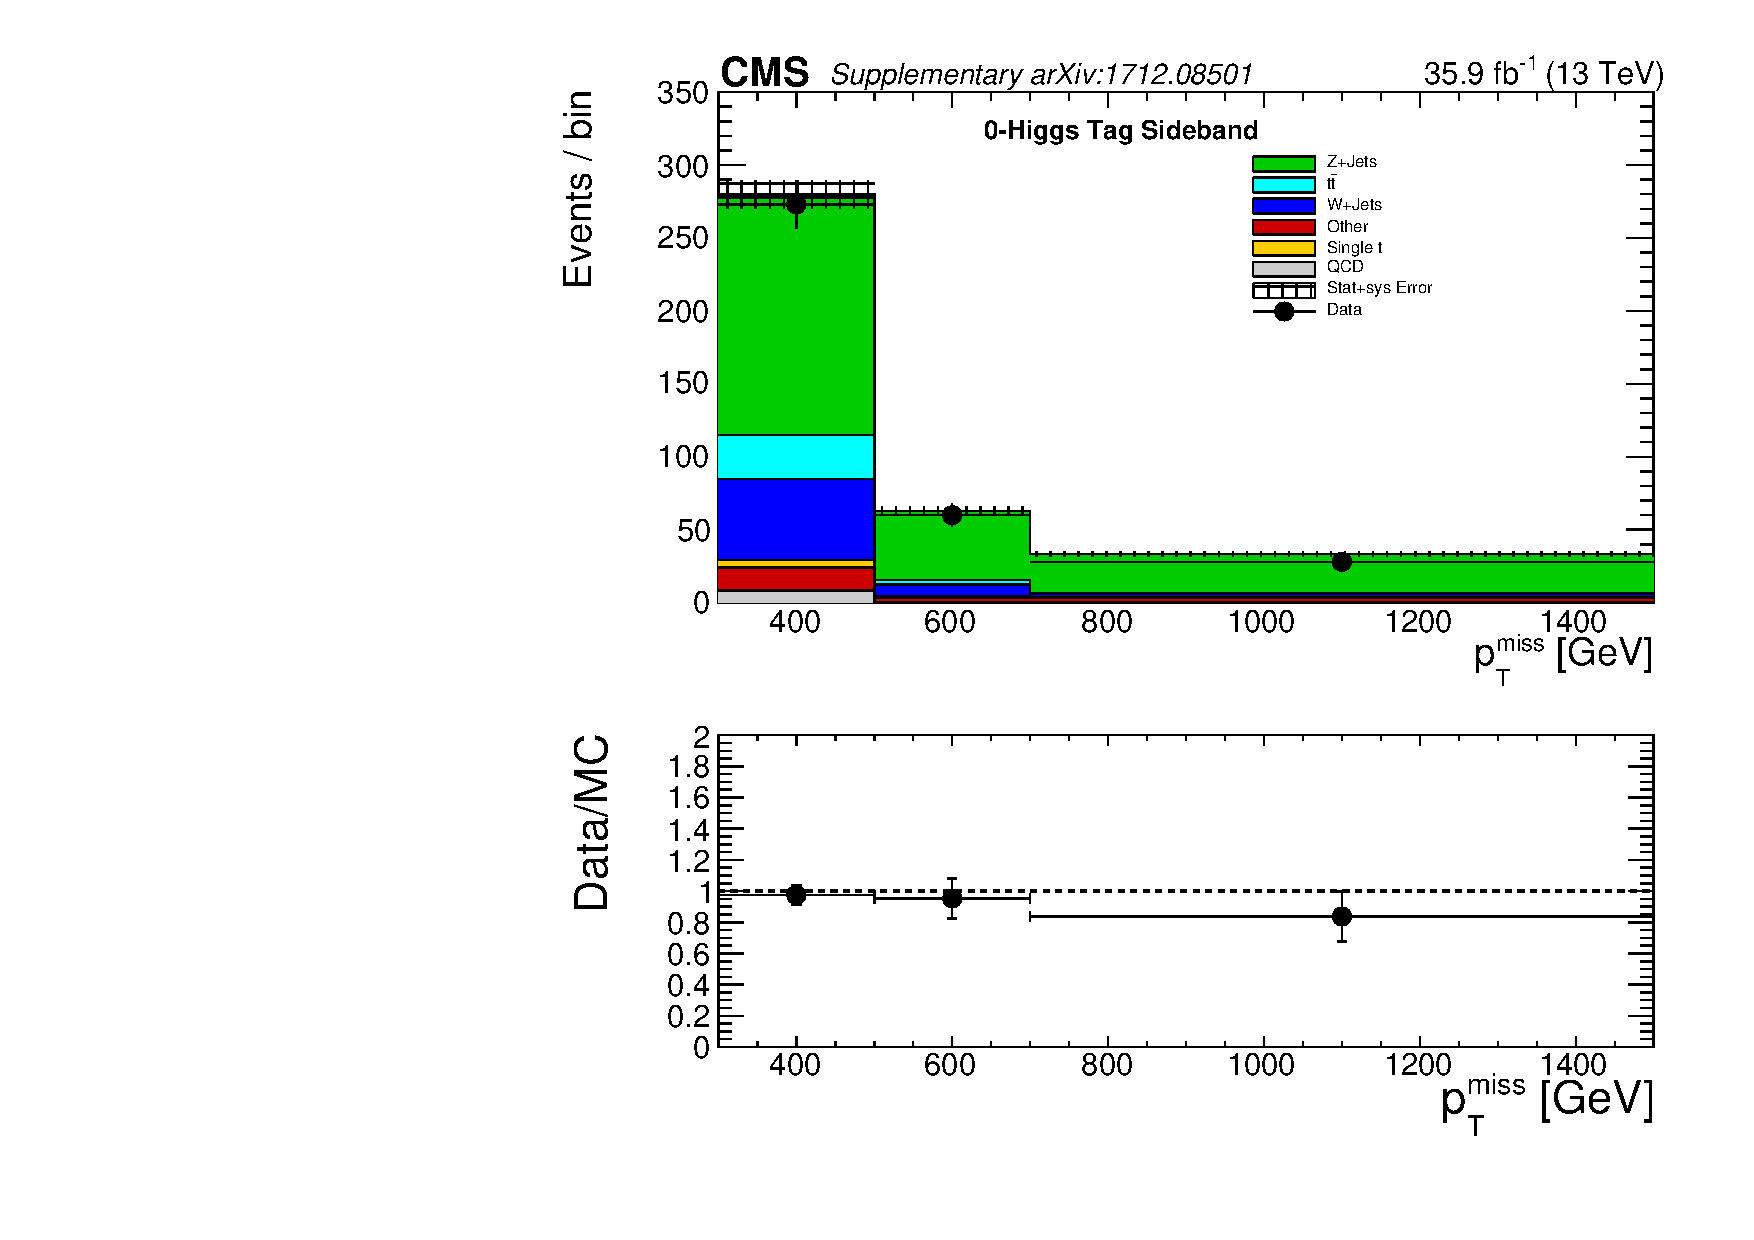
\includegraphics[trim={5px 5px 5px 5px},clip,width=0.425\linewidth]{figs/Unblinding_antitagSB.pdf}
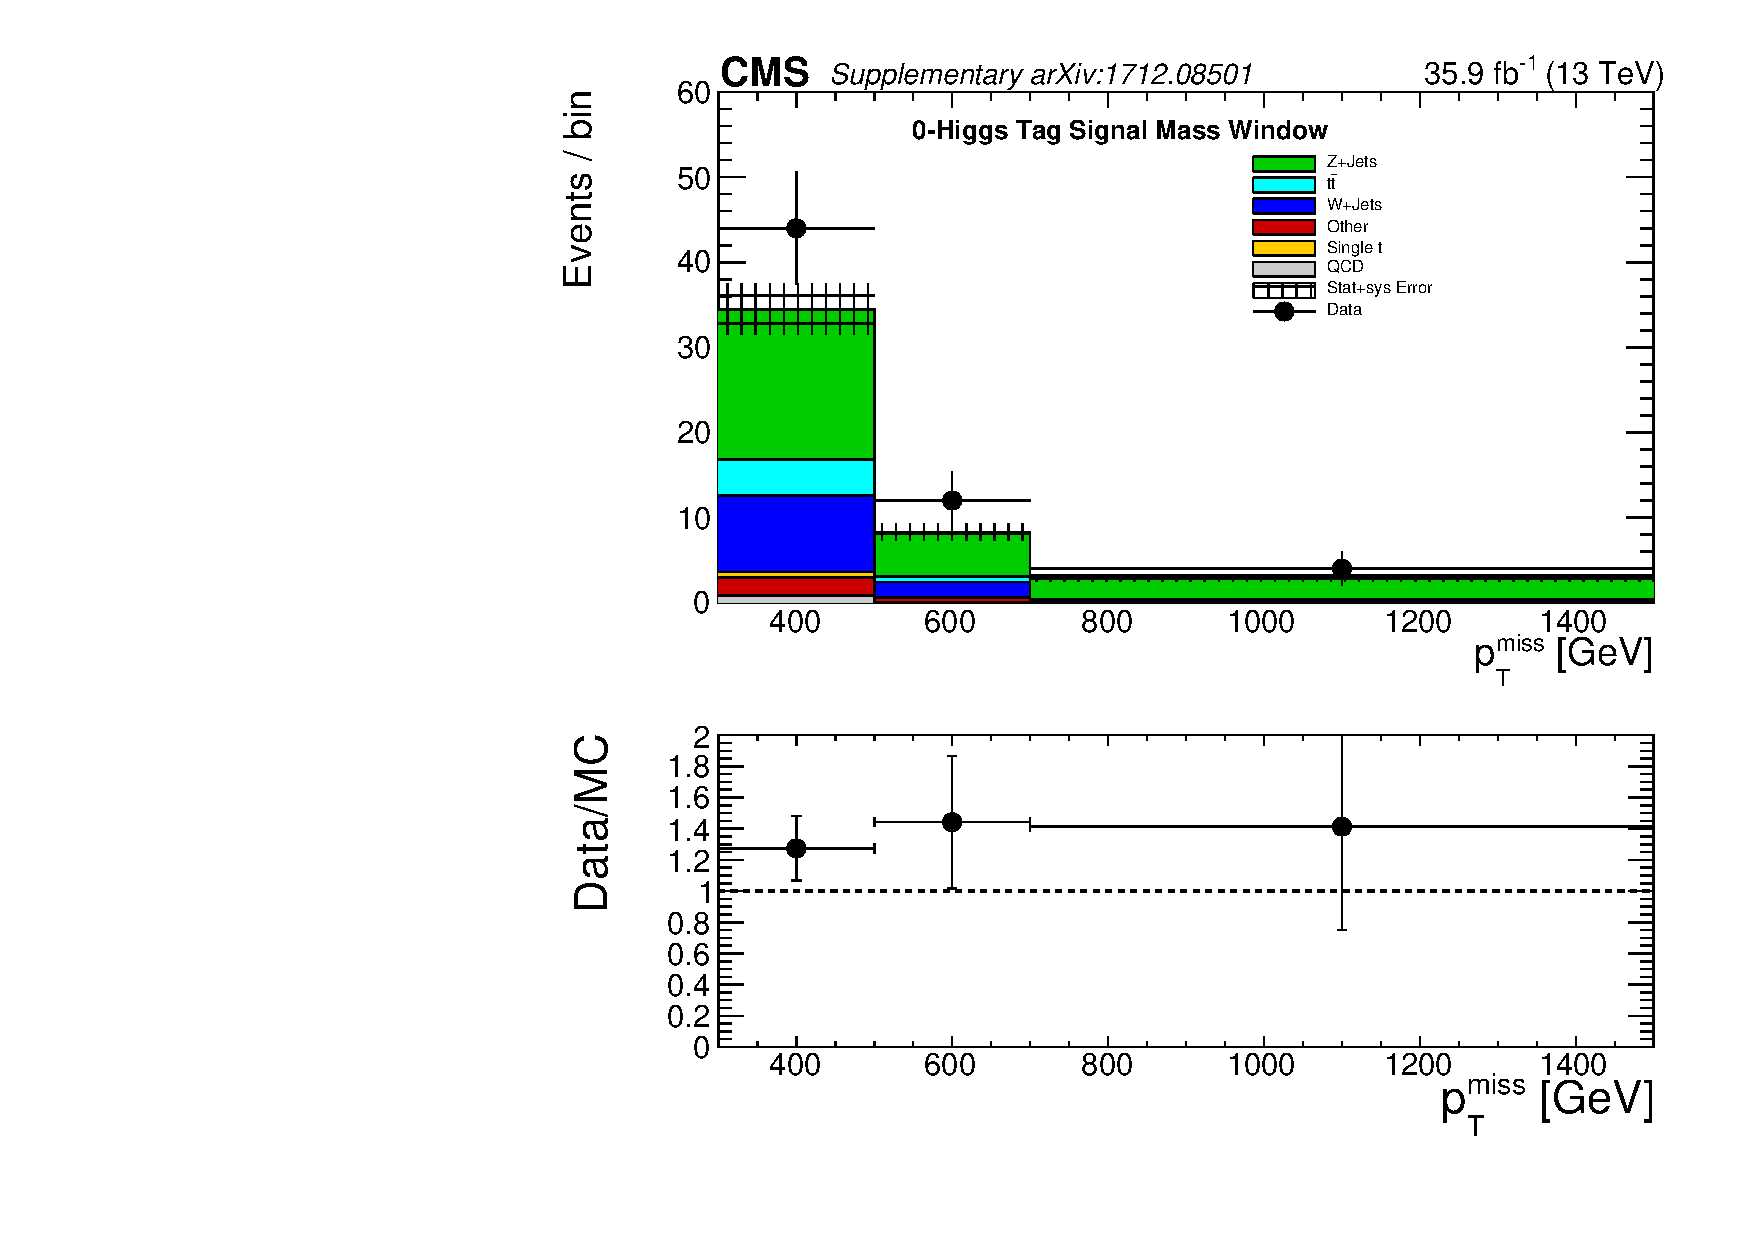
\includegraphics[trim={5px 5px 5px 5px},clip,width=0.425\linewidth]{figs/Unblinding_antitagSR.pdf}\\
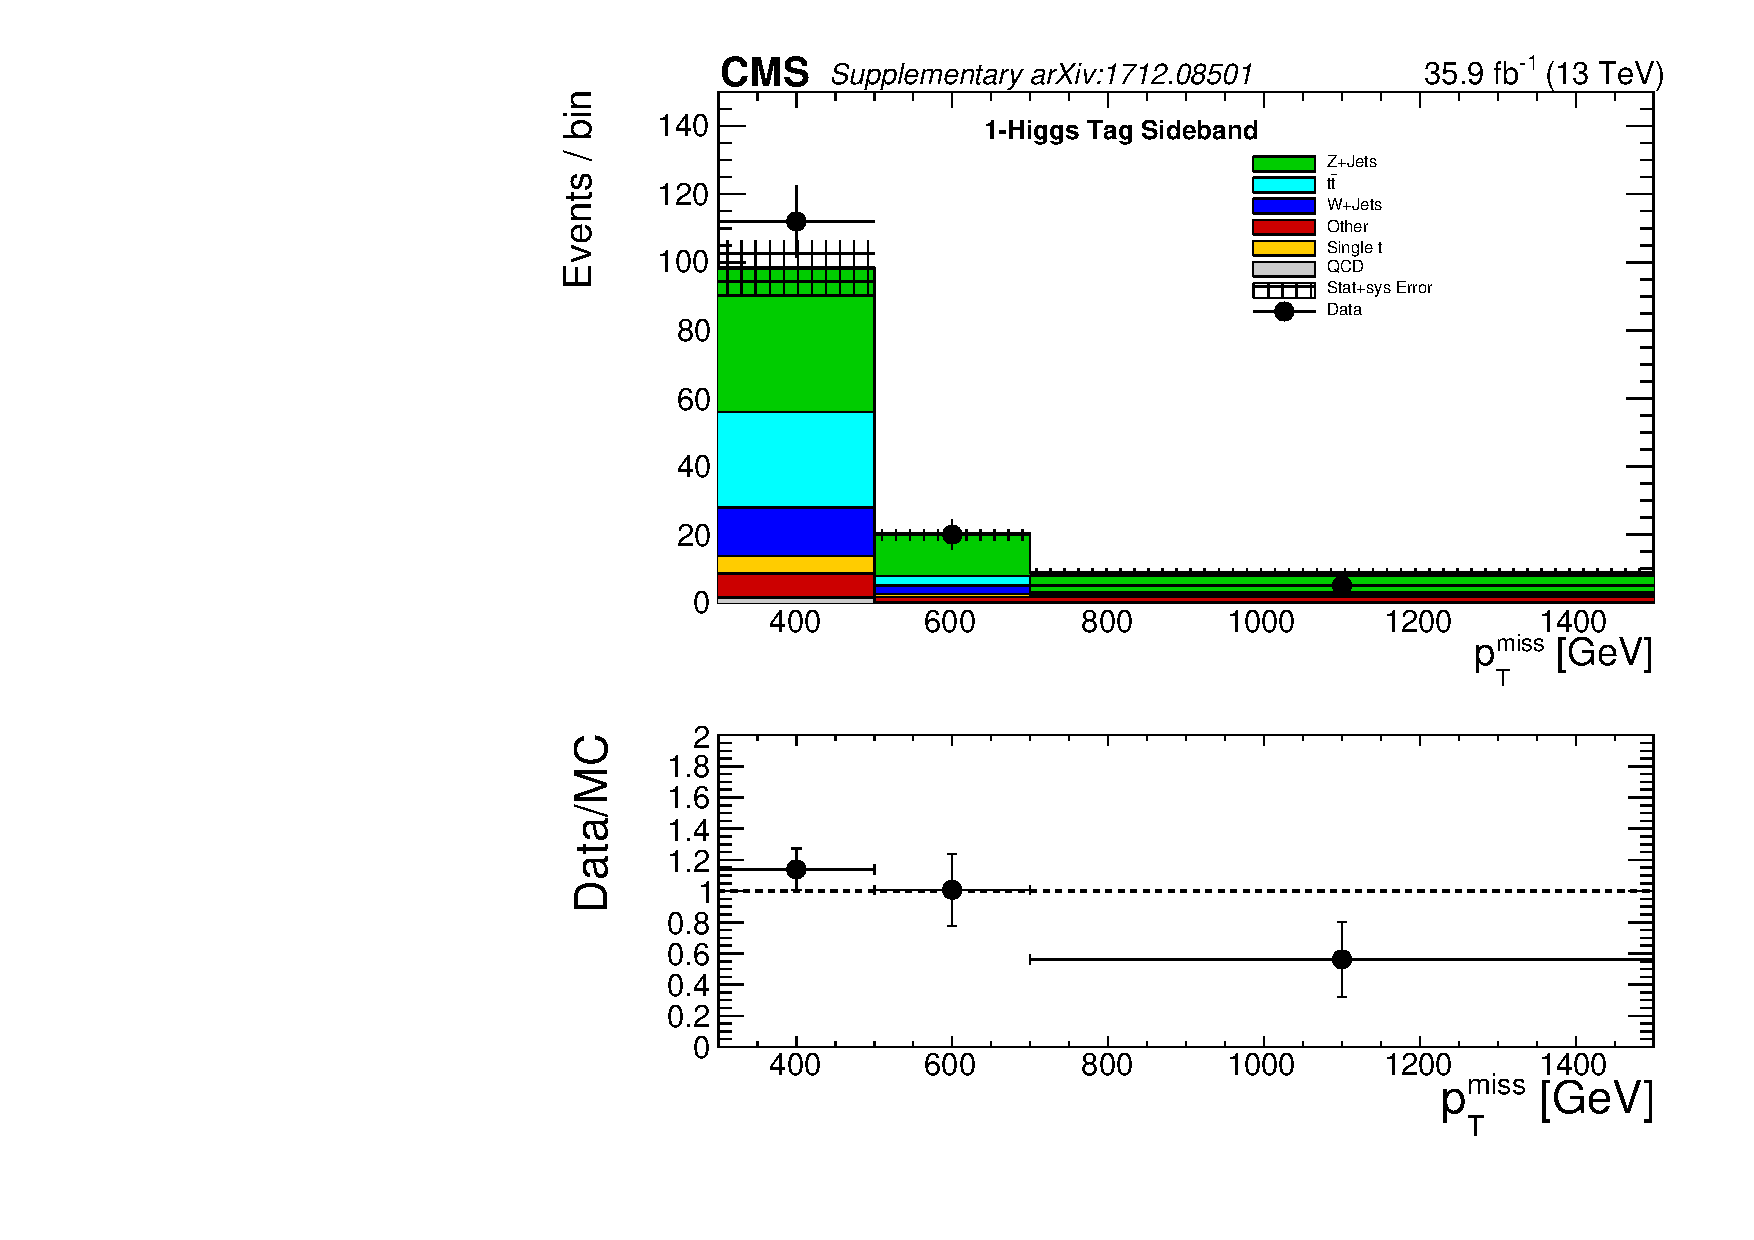
\includegraphics[trim={5px 5px 5px 5px},clip,width=0.425\linewidth]{figs/Unblinding_tagSB.pdf}
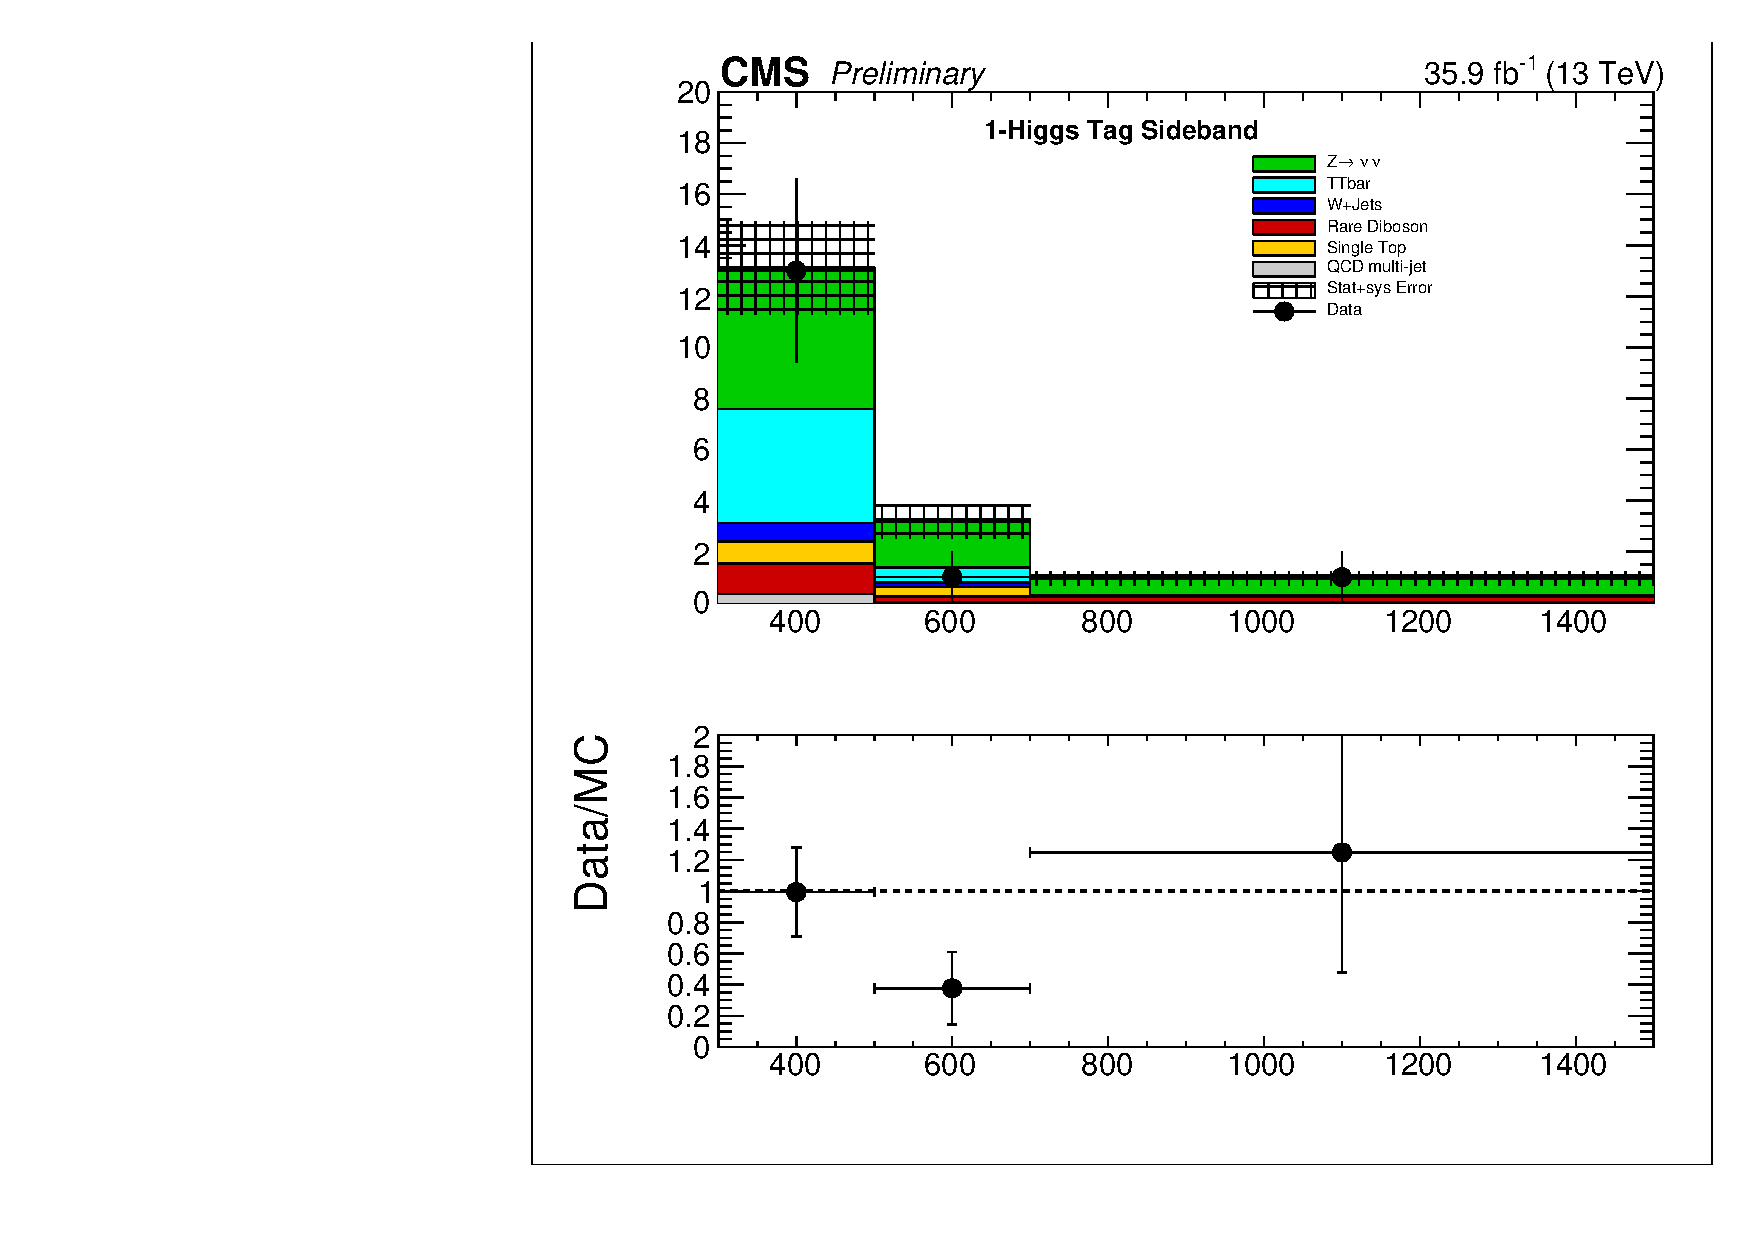
\includegraphics[trim={5px 5px 5px 5px},clip,width=0.425\linewidth]{figs/Unblinding_doubletagSB.pdf}\\
\caption
[Control region \ptmiss distributions comparing data and scale-factor corrected simulation.]{Control region \ptmiss distributions comparing data and scale-factor corrected simulation. The hashed red distribution denote the prediction from simulation; the solid points denote the observed yields in data.}
\label{fig:UnblindCR}
\end{figure}

\begin{table}[hbp!]
\centering
\caption{
Sideband region yields, $\kappa$, and background predictions for the 6 signal bins.
}
\begin{tabular}{lllllll}
\hline
\hline
$N_{\mathrm{H}}$ & $p_{T}^{\mathrm{miss}}$ (GeV) & B & C & D & $\kappa$  & $\kappa \cdot B \cdot C / D$ \\
\hline
$A_{1}$ & [300, 500 GeV]      & 112 & 44  & 273 & 0.98 $\pm$ 0.11 & 17.7 $\pm$ 3.8\\
$A_{1}$ & [500, 700 GeV]      & 20   & 12  & 60   & 0.86 $\pm$ 0.16 & 3.4  $\pm$ 1.5\\
$A_{1}$ & [700, $\infty$ GeV] & 5    & 4    & 28   & 0.86 $\pm$ 0.17 & 0.61 $\pm$ 0.45\\
$A_{2}$ & [300, 500 GeV]      & 13   & 44  & 273 & 0.73 $\pm$ 0.14 & 1.52 $\pm$ 0.57\\
$A_{2}$ & [500, 700 GeV]      & 1     & 12  & 60   & 0.43 $\pm$ 0.12 & 0.09 $\pm$ 0.08\\
$A_{2}$ & [700, $\infty$ GeV] & 1     & 4     & 28   & 0.62 $\pm$ 0.30 & 0.09$^{+0.11}_{-0.09}$\\
\hline
\hline
\end{tabular}
\label{tab:tab}
\end{table}

\section{Signal Systematics}
\label{sec:signalsys}
We consider a variety of systematic uncertainties on the signal efficiency and distribution. Some are common to more 
inclusive SUSY analyses \cite{RA2b:Moriond} and there are additional systematics related to $b\bar{b}$ tagging efficiency and 
the effect of the pruned mass scale and resolution on the signal efficiency.  
\begin{itemize}
\item {\bf Luminosity:} The recommendation for the 2016 dataset is currently a flat uncertainty of 2.5\%.
\item {\bf Isolated track veto:} A flat uncertainty of 2\% is assigned to the signal samples to account for any data/MC differences based on the study from the 2015 analysis \cite{RA2b:Moriond}.
\item {\bf MC statistics:} The signal MC sample statistical uncertainty is generally 2-4\% .
\item {\bf Trigger efficiency:} The effect of the uncertainty on the signal yield is about 2\%.
\item {\bf Pileup reweighting:} The sensitivity to the pileup distribution was studied for various benchmark signal models by comparing events with $n_{\textrm{vtx}} < 20$ (low PU) or $n_{\textrm{vtx}} \geq 20$ (high PU). Accordingly, no pileup reweighting is applied to the signal MC samples and no associated uncertainty is assessed.
\item {\bf ISR:} An ISR correction is derived from tt events, with a selection requiring two lep-
tons (electrons or muons) and two b-tagged jets, implying that any other jets in the
event arise from ISR. The correction factors are 1.000, 0.920, 0.821, 0.715, 0.662, 0.561,
0.511 for NISR = 0, 1, 2, 3, 4, 5, 6+. The corrections are applied to the simulated signal jet
samples with an additional normalization factor, typically ∼1.15 (depending on the signal model), to ensure the overall cross section of the sample remains constant. The systematic uncertainty in these corrections is chosen to be half of the deviation from unity for each correction factor. The effect on the yield ranges from $0.0–1\%$, with the largest effect at high MET.
\item {\bf Scales:} The uncertainty is calculated using the envelope of the weights from varying the renormalization and factorization scales, $\mu_{R}$ and $\mu_{F}$,by a factor of 2 \cite{Cacciari:2003fi, Catani:2003zt}. The effect on the yield of is less than 0.1\%.
\item {\bf Jet Energy Corrections:} The jet energy corrections (JECs) are varied using the $p_{T}$-
and $\eta$-dependent jet energy scale uncertainties from the official database.
These variations are propagated into the various jet-dependent variables, including: HT, MET, $\Delta\phi(\textrm{MET},j_{i})$.
The overall effect is less than 1\%.
\item {\bf Jet Energy Resolution:} The jet momenta in the MC samples are smeared to match the jet energy resolution in data. The smearing factors are varied according to the uncertainties on the jet energy resolution measurements.
These variations are propagated into the various jet-dependent variables, including: HT, MET, $\Delta\phi(\textrm{MET},j_{i})$.
The overall effect ranges from 0.01\%.
\item {\bf PDFs:} The LHC4PDF prescription for the uncertainty on the total cross section is included as $\pm 1$ sigma bands in the results plots. No
additional uncertainty is considered for the uncertainty in the acceptance due to PDFs, as per SUSY group recommendation.
\end{itemize}
The above signal systematics are applied as an uncertainty on the signal normalization. These uncertainties are in general small. The main signal systematics 
come from the AK8 Jet Double-b tagging efficiency data/MC scale factors and the uncertainty on the pruned mass resolution.
The AK8 Jet Double-b tagging efficiency has an uncertainty which is propagated to the signal efficiency. This uncertainty is applied 
as a shape uncertainty across the Higgs tag regions and the anti-tag region. Also the pruned jet mass scale and resolution uncertainties are 
propogated to the final signal efficiency using POG recommendations. The pruned mass scale factor is derived using W-jets in semi-leptonic \ttbar and extrapolating to the H mass. This uncertainty is assigned a shape uncertainty on the signal mass window and the sideband. \\
\begin{itemize}
\item A data/MC scale-factor is derived from double-muon tag data selected with HLT Trigger \texttt{HLT\_BTagMu\_AK8Jet300\_Mu5\_v} and muon enriched QCD Monte-Carlo. The scale factors have mainly a statistical error along with a smaller set of systematic errors due to shape systematics, Jet-Energy scale uncertainty, Pile-up corrections, uncertainty on the number of tracks, uncertainty of b-fragmentation and  c-fragmentation, and the uncertainty on $K_{s}$ and $\Lambda$ fraction. 
\item The pruned mass scale-factor is derived by comparing the efficiency to select W-jets in data and MC within a mass window of $\left[65,85\right]$ GeV.  The fit for the gaussian resolution of the W-mass peak is shown in Figure~\ref{fig:WMassPeak} and the fit results are shown in Table~\ref{tab:WMassFit}. The mass scale between MC and data is consistent though MC predicts a narrower mass resolution compared to data. The jet mass in each event is smeared to mimic the pruned jet mass resolution in data and an uncertainty is assigned based on the ratio of efficiencies between the smeared and un-smeared cases~\cite{CMS_AN_2016-215}.
\end{itemize} 

The summary of the signal systematics and their effect on the signal yields is shown in Table~\ref{tab:SignalSystSummary}. The dominant effect is from the mass resolution uncertainty.
%\item The pruned mass scale-factor is found to be consistent with 1.0 for the pruned mass-scale with an uncertainty based on the Jet-Energy scale uncertainty: $\sqrt{JES^2 + 0.02^2}$. The pruned jet mass-resolution scale-factor is found to $7\%$ with an uncertainty of $\sqrt{JER^2+0.103^2}$


\begin{figure}[hbp!]
\begin{center}
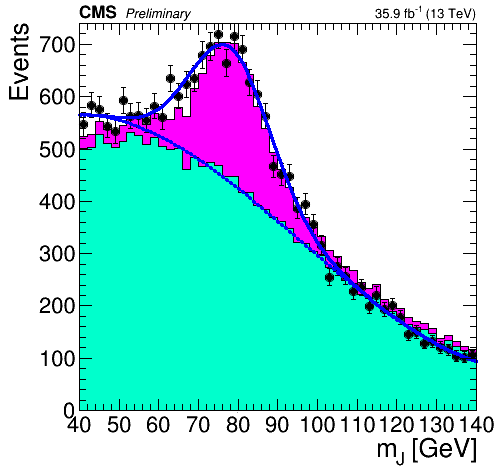
\includegraphics[width=0.5\linewidth]{figs/WMassPeakDataMC.png}
\end{center}
\caption
[Pruned jet mass in semi-leptonic \ttbar events.]
{Pruned jet mass in semi-leptonic \ttbar events. The mass peak for the W-jets is used to derive the mass resolution uncertainty.}
\label{fig:WMassPeak}
\end{figure}

\begin{table}[hbp!]
\centering
\begin{tabular}{c|c}
\hline \hline
\multicolumn{2}{c}{Data}\\
\hline \hline 
Mean &  $78.2 \pm 0.46$\\ \hline
Sigma & $10.10  \pm 0.671$ \\ \hline
\hline
\multicolumn{2}{c}{\ttbar MC}\\ \hline
\hline
Mean &  $ 78.4  \pm 0.35$\\ \hline
Sigma & $ 7.23   \pm 0.48$ \\ \hline
\end{tabular}
\caption{Fit results for W-mass resolution in data and MC}
\label{tab:WMassFit}
\end{table}

\begin{table}[hbp!]
\centering
\begin{tabular}{c|c}
\hline \hline
\multicolumn{2}{c}{Unc. on Normalization} \\  \hline
\hline \hline
Systematic & \% Effect on yields\\ \hline
Luminosity & 2.6\% \\ \hline
Trigger Eff. & 2.0\% \\ \hline
Iso. Track Veto & 2\%\\ \hline
ISR modeling & 0.01\% \\ \hline
PDF Scale & 0.1\% \\ \hline
JEC & 1\% \\ \hline
JER & 0.01\% \\ \hline
MC Stat & 1-4\% \\ \hline
\multicolumn{2}{c}{Shape Unc.} \\  \hline
Double-b SF & 6\% \\ \hline
Mass Resolution &1-15\% \\ \hline
\hline
\end{tabular}
\caption{
    Summary of signal shape and normalization uncertainties. 
}
\label{tab:SignalSystSummary}
\end{table}

\section{Results - Yields in the Signal Regions \& Exclusion Curves}
\label{sec:results}

After unblinding the 4x3=12 sideband regions and performing the background estimation the 2x3=6 signal regions were unblinded. The observed yields, along with the SM background predictions, are seen in Table~\ref{tab:DataPred}. Our signal region yields are consistent with the SM background expectation. Additionally, Table~\ref{tab:DataPred} shows the expected signal yields for two model points corresponding to gluino $\tilde{g}$ masses of 2000 or 1800 GeV; the mass of the neutralino $\tilde{\chi}_{1}^{0}$ is fixed at 1 GeV; the mass splitting between the gluino $\tilde{g}$ and neutralino $\tilde{\chi}_{2}^{0}$ is fixed at 50 GeV.

\begin{table}[hbp!]
\caption{Signal yields and SM background predictions}
\centering
\begin{tabular}{l|c|c|c|c||c|c|}
\hline \hline
\ptmiss & $B \cdot C / D$ & $\kappa$ & $\kappa \cdot B \cdot C / D$ & Obs. & T5HH(2000) & T5HZ(1800) \\
\hline \hline
\multicolumn{7}{c}{1-Higgs Tag} \\ \hline \hline
[300, 500 GeV]      & $18.05 \pm 3.39$  & $0.98 \pm 0.11$ & $17.68 \pm 3.85$ & 15 & 0.24 & 0.75  \\ \hline
[500, 700 GeV]      & $4 \pm 1.54$ & $0.86 \pm 0.16$ & $3.44\pm 1.47$ &  2  & 0.32 & 0.98 \\\hline
[700, $\infty$ GeV] &  $0.71 \pm 0.50$  &  $0.86 \pm 0.17$ & $0.61\pm 0.45$ &  1 & 2.13 & 4.34\\\hline \hline
\multicolumn{7}{c}{2-Higgs Tag} \\  \hline \hline
[300, 500 GeV]       &   $2.09 \pm 0.67$  & $0.73 \pm 0.14$ & $1.52 \pm 0.57$ & 1 & 0.17 & 0.35\\ \hline
[500, 700 GeV]       & $ 0.2 \pm 0.20$ & $0.43 \pm 0.12$ &$0.09^{+0.08}_{-0.08}$ & 0 & 0.23 & 0.44\\ \hline
[700, $\infty$ GeV] & $0.14 \pm 0.16$ & $0.62 \pm 0.30$ & $0.09^{+0.11}_{-0.09}$ & 0 & 1.36 & 1.98\\ \hline
\hline
\end{tabular}
\label{tab:DataPred}
\end{table}

A visual representation of the one event in the double-H tagged signal bin is seen in Figure~\ref{fig:fireworks}. The purple line represents \ptmiss=426 GeV. The three yellow cones represent the AK8 jets labeled with $p_{T}$.  Note the two additional objects not satisfying our object definition but still plotted in the representation a) the additional low-$p_{T}$ and low mass AK8 jet b) the $p_{T}$=18 GeV muon (red line) suffers from poor reconstruction properties.

\begin{figure}[hbp!]
\centering
\begin{subfigure}[b]{0.49\textwidth}
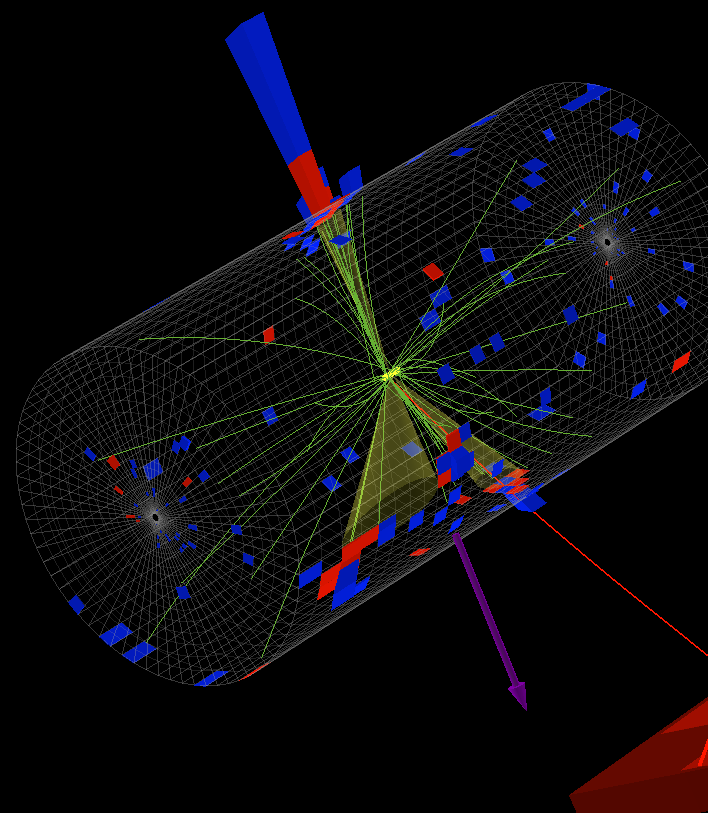
\includegraphics[width=\textwidth]{figs/fireworks_ak8barrel.png}
\end{subfigure}
\begin{subfigure}[b]{0.49\textwidth}
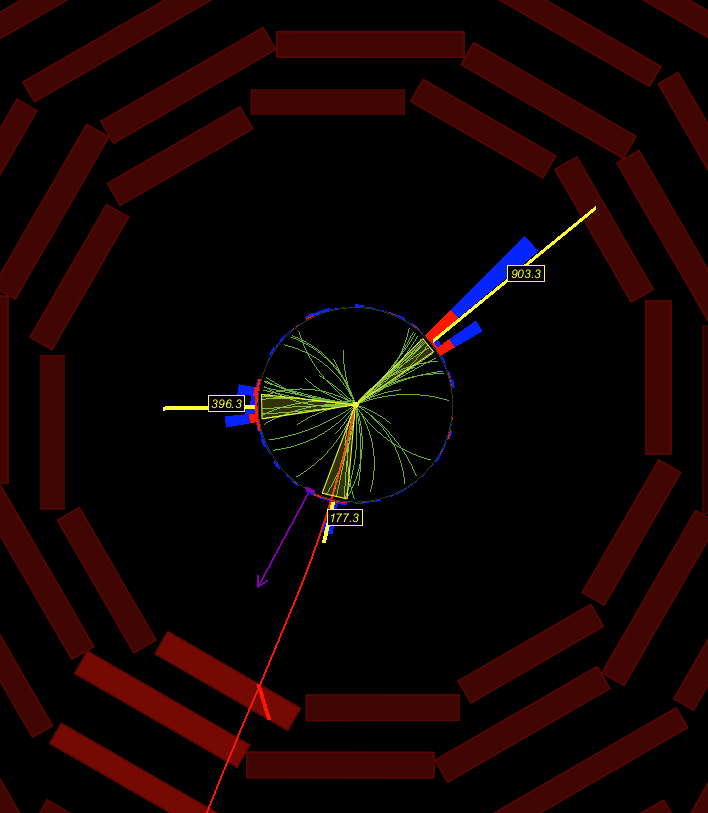
\includegraphics[width=\textwidth]{figs/fireworks_ak8rhophi.png}
\end{subfigure}
\caption{The single event in the $A_{2}$ region.}
\label{fig:fireworks}
\end{figure}

Interpreting our results in the context of the T5HH or T5ZH models, the absence of signal allows us to place lower limits on the mass of the gluino $\tilde{g}$. For the statistical treatment, we use the Higgs combination tool to encode the ABCD approach in the likelihood. In this approach, the data card for one search bin contains the observed number of events and the expected signal and background in each of the ABCD regions. A likelihood function is built that contains these ABCD regions and explicitly encodes the relation $A=\kappa B \frac{C}{D}$ and a Gaussian nuisance is assigned for the uncertainty on $\kappa$. The likelihood for each search bin can be described by:

\begin{equation}
\mathcal{L}=\prod^{ABCD}_{i} Poisson\left(n_i \vert bkg_i + r\cdot sig_i\right) \times \prod^{nuisances}_j Constraints\left(\theta_j , \hat{\theta}_j\right)
\end{equation}

where the 4 regions are modeled by Poisson distribution and the term Constraints refers to either Gaussian distributions for the $\kappa$ uncertainties or log normal distributions that model the signal systematics. The expected and observed limits are then calculated based on the asymptotic approximation of the profile likelihood ratio using the CLs criterion to place limits at the $95\%$ confidence level. These exclusion curves are seen in Figure~\ref{fig:brazil}. We are able to place lower limits at 95\% confidence level on the gluino $\tilde{g}$ mass at 2010 and 1825 GeV for the T5HH and T5ZH models, respectively. The weaker limit for the T5ZH model is due to the smaller branching fraction of the Z boson to b-quarks and our choice of signal mass window not being optimal for Z reconstruction.

\begin{figure}[hbp!]
\centering
\begin{subfigure}[b]{0.49\textwidth}
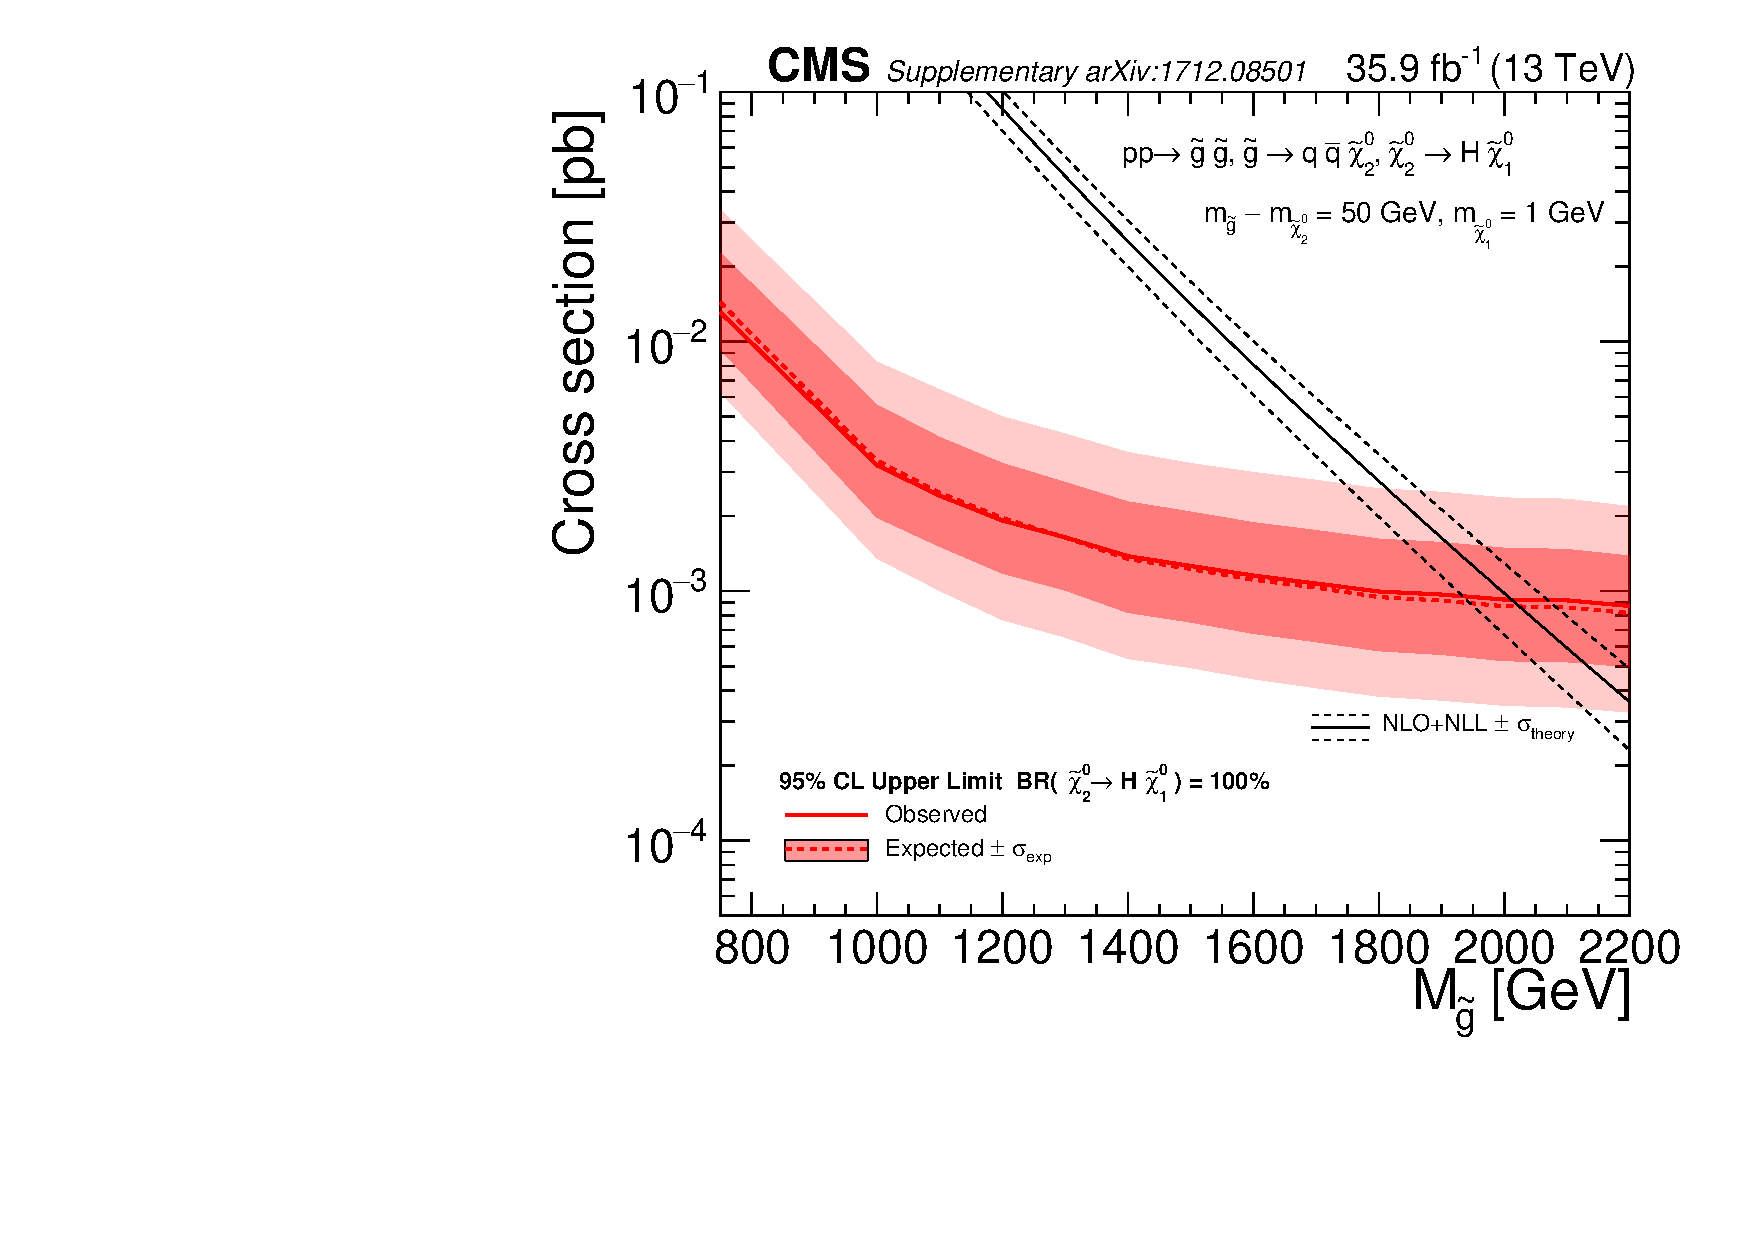
\includegraphics[width=\textwidth]{figs/brazilT5HHResults.pdf}
\caption{T5HH}
\end{subfigure}
\begin{subfigure}[b]{0.49\textwidth}
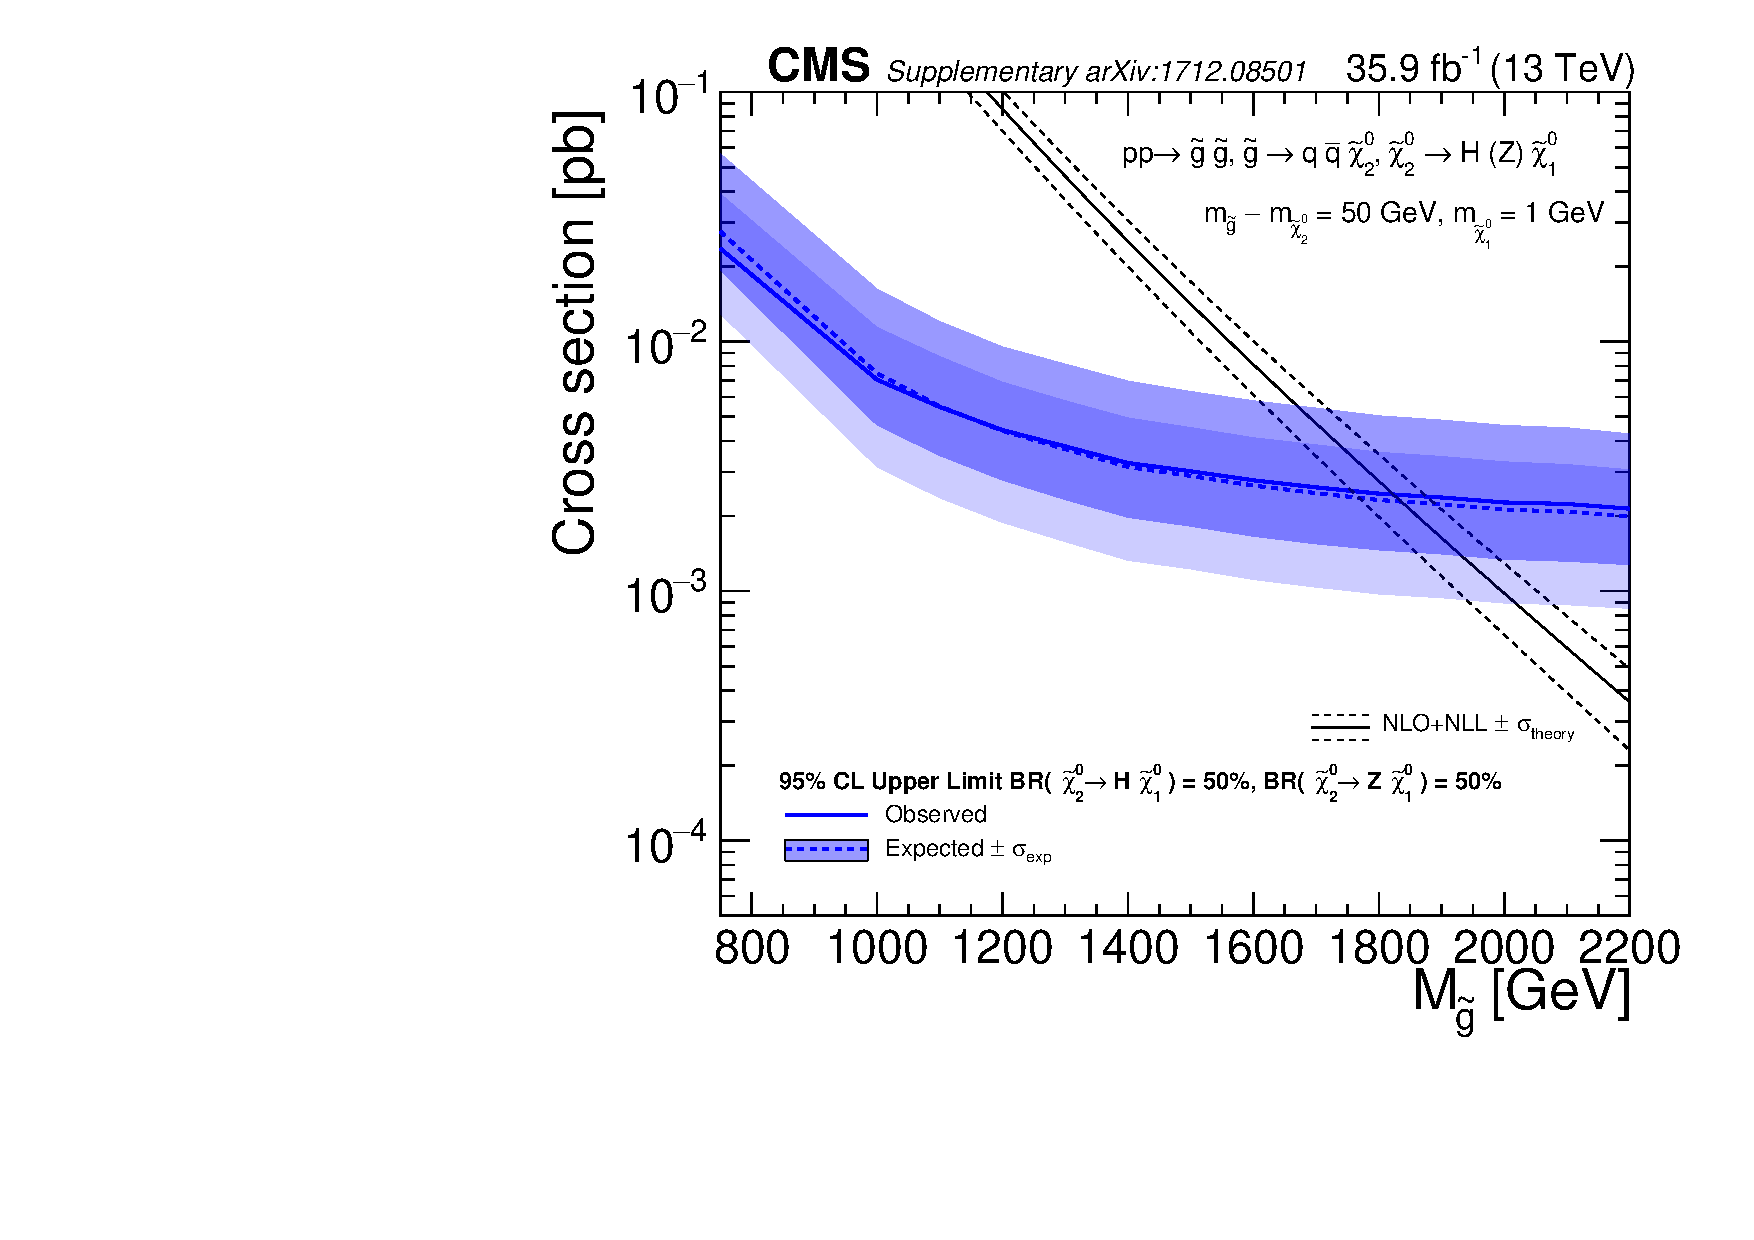
\includegraphics[width=\textwidth]{figs/brazilT5HZResults.pdf}
\caption{T5ZH}
\end{subfigure}
\caption{Observed and expected limits on the gluino cross section.}
\label{fig:brazil}
\end{figure}

\section{Reinterpretation}
\label{sec:reinterpretation}

In Section~\ref{sec:results} our results were presented in the context of limit-setting for the T5HH and T5ZH models. Many such SMS models exist within the MSSM which predict the production of high-$p_{T}$ bosons and it is therefore important to include information necessary to make predictions of yields for different final states. This is aided by providing the user with efficiencies for $b\bar{b}$ tagging and mass tagging of the AK8 jets. Tagging efficiencies for the five largest decay channels relevant to the analysis for the H boson are seen in \ref{fig:effH}. Tagging efficiencies for the hadronic decay modes of the Z boson are seen in Figure~\ref{fig:effZ}, the much lower mass tagging efficiency for the Z boson is due to our choice of signal mass window [85, 135 GeV] not being optimal for Z boson reconstruction. These are used to calculate the expected yields in the 6 analysis regions when performing a reinterpretation of the analysis using different final states. 

For each event, the yield in each bin can be predicted by first forming the following weights using the tagging efficiencies for the leading two jets, as seen below. j0 and j1 represent the leading and subleading AK8 jet, respectively. The weights on the right-hand-side are $p_{T}$ dependent.

\begin{itemize}
\item double mass tag weight = $j0_{signalmass} \cdot j1_{signalmass}$
\item anti mass tag weight = $(j0_{sidebandmass} \cdot j1_{signalmass}) + (j1_{signalmass} \cdot j1_{sidebandmass}) + (j0_{sidebandmass} \cdot j1_{sidebandmass})$
\item double bb tag weight = $j0_{bbtag} \cdot j1_{bbtag}$
\item single bb tag weight = $(j0_{bbtag} \cdot (1-j1_{bbtag})) + ((1-j0_{bbtag})\cdot j1_{bbtag})$
\item anti bb tag weight = $(1-j0_{bbtag}) \cdot (1-j1_{bbtag}$)
\end{itemize}

These weights are then combined in the following manner to determine the yields across each of the 6 bins for a single event.

\begin{itemize}
\item A1 weight = (single bb tag weight) $\cdot$ (double mass tag weight)
\item A2 weight = (double bb tag weight) s$\cdot$ (double mass tag weight)
\item B1 weight = (single bb tag weight) $\cdot$ (anti mass tag weight)
\item B2 weight = (double bb tag weight) $\cdot$ (anti mass tag weight)
\item C weight = (anti bb tag weight) $\cdot$ (double mass tag weight)
\item D weight = (anti bb tag weight) $\cdot$ (anti mass tag weight)
\end{itemize}

These weights for the 6 analysis bins (inclusive in \ptmiss) are then summed over all events to get the expected yields.
Following this prescription, the authors performed this prediction using the T5HH model with a gluino mass of 2200 GeV and compared to the true value.
The largest deficit was in the D region, with a difference of -36\% difference from nominal.
The greatest over-prediction is found in the B2 region, with a surplus of +8.2\% events relative to nominal.
The closure in the other bins fall somewhere in this range.
These results are summarized in Table~\ref{tab:predclos}.
As a further cross-check to the yield estimates, Table~\ref{tab:sigeff} shows the true signal event efficiencies for the T5HH model with a gluino mass of 2200 GeV.

\begin{figure}[hbp!]
\centering
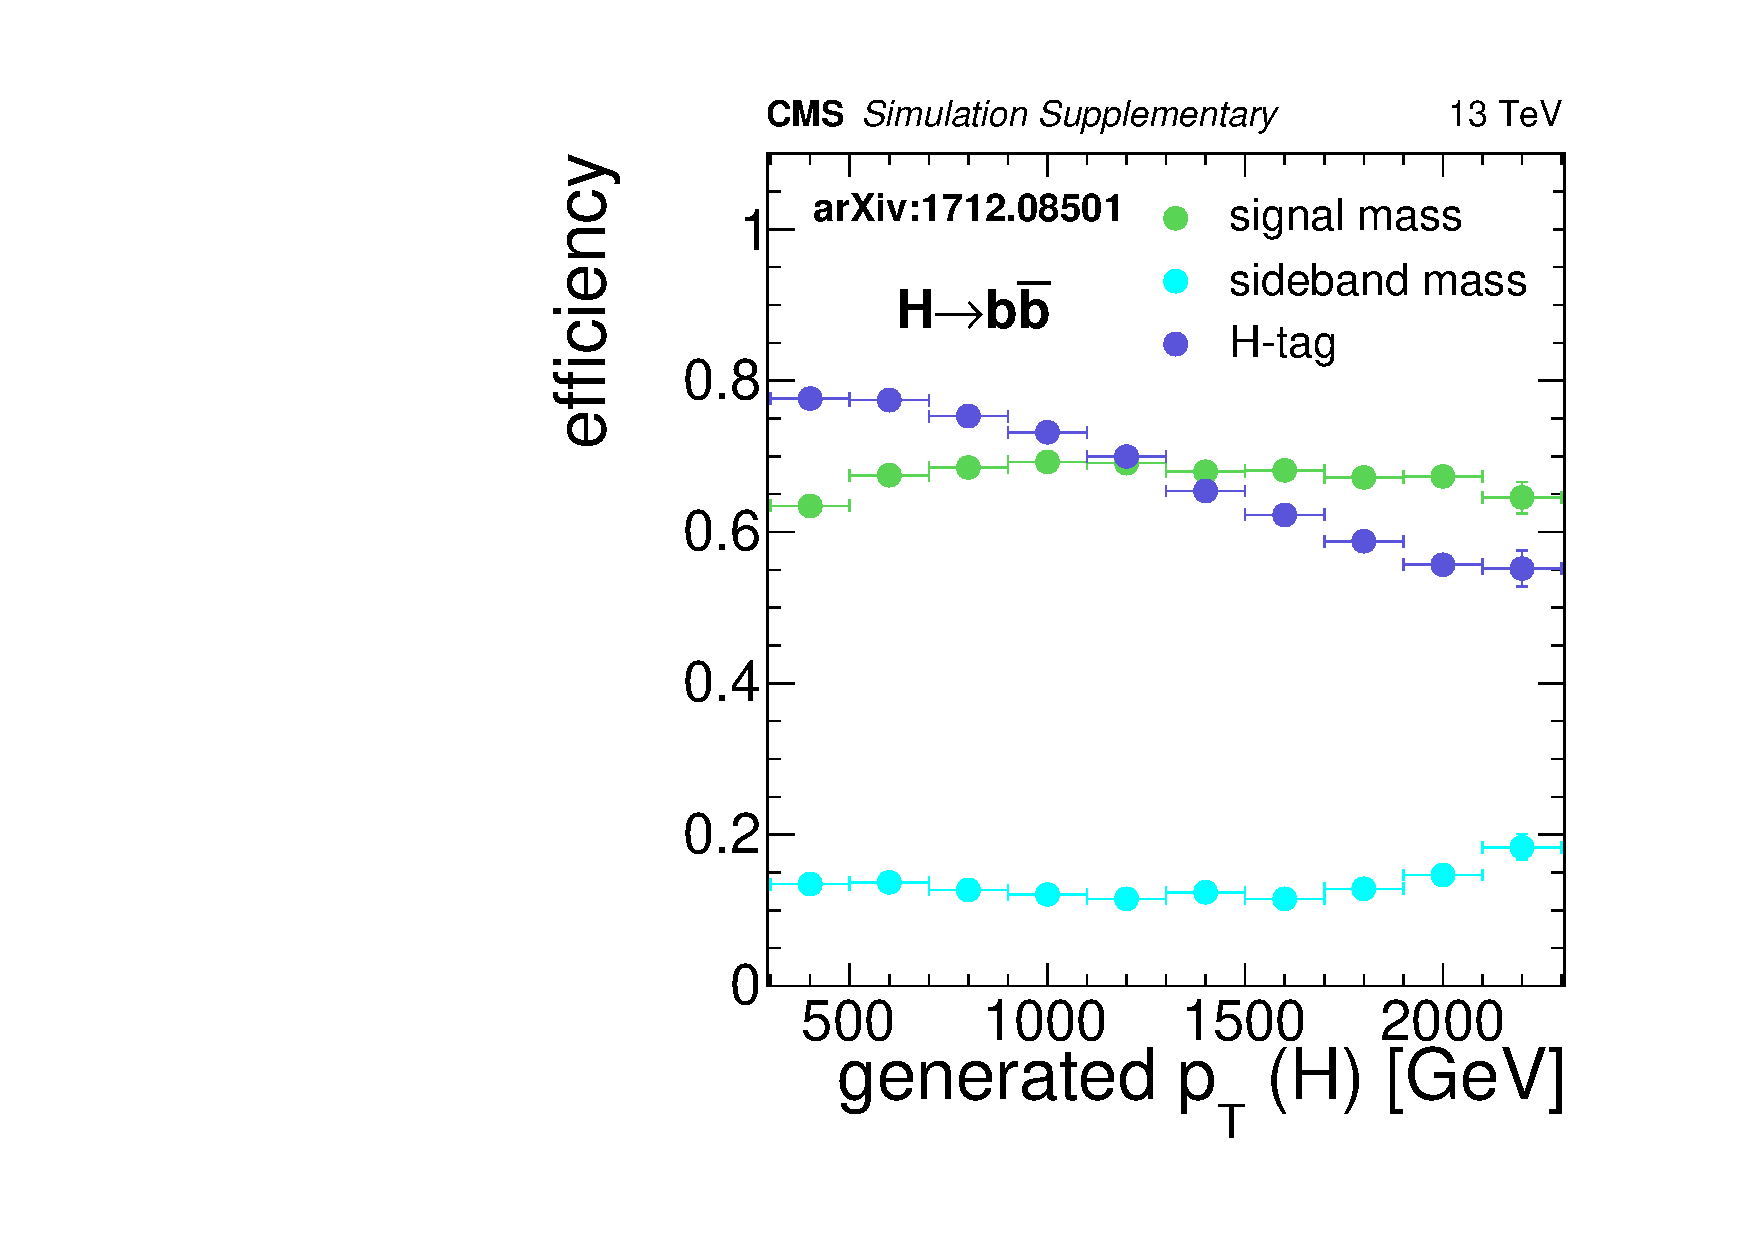
\includegraphics[width=0.425\linewidth]{figs/CMS-SUS-17-006_Figure-aux_006.pdf}
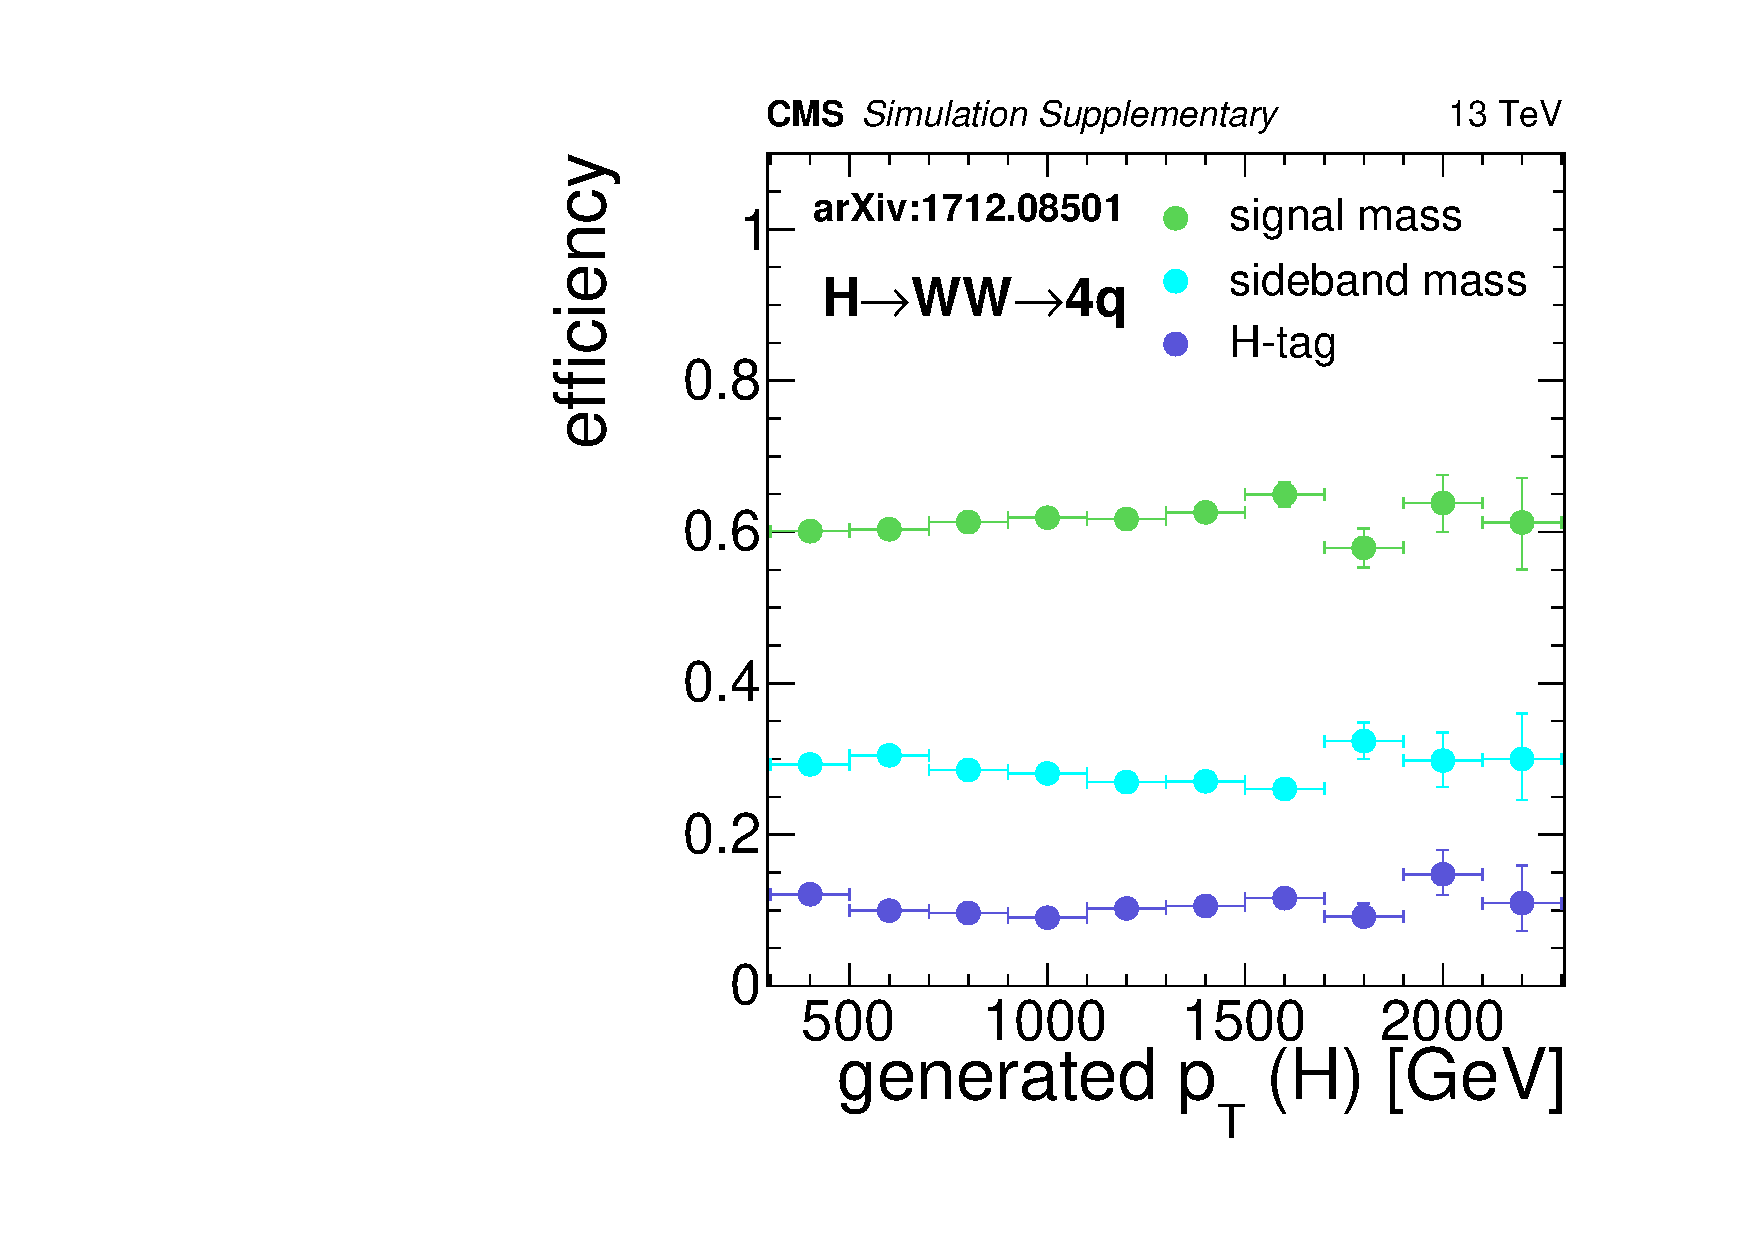
\includegraphics[width=0.425\linewidth]{figs/CMS-SUS-17-006_Figure-aux_007.pdf}
\includegraphics[width=0.425\linewidth]{figs/CMS-SUS-17-006_Figure-aux_008.pdf}
\includegraphics[width=0.425\linewidth]{figs/CMS-SUS-17-006_Figure-aux_009.pdf}
\includegraphics[width=0.425\linewidth]{figs/CMS-SUS-17-006_Figure-aux_010.pdf}
\includegraphics[width=0.425\linewidth]{figs/blankcanvas.pdf}
\caption[Efficiencies for an AK8 jet originating from H boson decay, relative to baseline selection.]{
Efficiencies for an AK8 jet originating from H boson decay, relative to baseline selection.
"signal mass" represents the probability the jet will have mass [85, 135 GeV].
"sideband mass" represents the probability the jet will have mass [50, 85 GeV] or [135, 250 GeV].
"H-tag" represents the probability the jet have a double-b discriminator value greater than 0.3, for jets with mass [50, 250 GeV].
Efficiencies were derived using the T5ZH MC with a gluino mass of 2200 GeV.
}
\label{fig:effH}
\end{figure}

\begin{figure}[hbp!]
\centering
\includegraphics[width=0.425\linewidth]{figs/CMS-SUS-17-006_Figure-aux_011.pdf}
\includegraphics[width=0.425\linewidth]{figs/CMS-SUS-17-006_Figure-aux_012.pdf}
\caption[Efficiencies for an AK8 jet originating from Z boson decay, relative to baseline selection.]{
Efficiencies for an AK8 jet originating from Z boson decay, relative to baseline selection.
"signal mass" represents the probability the jet will have mass  [85, 135 GeV].
"sideband mass" represents the probability the jet will have mass [50, 85 GeV] or [135, 250 GeV].
"H-tag" represents the probability the jet have a double-b discriminator value greater than 0.3, for jets with mass [50, 250 GeV].
Efficiencies were derived using the T5ZH MC with a gluino mass of 2200 GeV.
}
\label{fig:effZ}
\end{figure}

\begin{table}[hbp!]
\centering
\caption[Comparison of the true reco-level event yield with those obtained via the prediction.]{
Comparison of the true reco-level event yield with those obtained via the prediction. The columns with the RECO or GEN labels are the prediction using RECO or GEN event variables only, respectively. The prediction was made using the T5HH MC with a gluino mass of 2200 GeV.
}
\begin{tabular}{c | c c c}
\hline\hline
         & RECO     & RECO           & GEN\\
         & "truth"  & prediction     & prediction\\
\hline
Baseline & 4.08     & 3.46 (-15\%)   & 3.53 (-16\%)\\
A1       & 1.21     & 1.18 (-2.3\%)  & 1.26 (+3.6\%)\\
A2       & 0.777    & 0.748 (-3.7\%) & 0.815 (+4.7\%)\\
B1       & 0.802    & 0.703 (-12\%)  & 0.664 (-21\%)\\
B2       & 0.322    & 0.338 (+5.0\%) & 0.350 (+8.2\%)\\
C        & 0.498    & 0.473 (-4.9\%) & 0.487 (-2.1\%)\\
D        & 0.478    & 0.353 (25\%)   & 0.308 (-36\%)\\
\hline\hline
\end{tabular}
\label{tab:predclos}
\end{table}

\begin{table}[hbp!]
\centering
\caption[T5HH signal event efficiencies.]{
Signal efficiencies for an event to land in a given analysis bin.
The efficiencies were derived using the T5HH MC with a gluino mass of 2200 GeV.
Choosing a gluino mass of 1800 GeV decreases the efficiencies by a relative 5\%.
}
\begin{tabular}{c | c c c c c c c c}
\hline
\hline
                                                            & Baseline & A1     & A2      & B1      & B2      & C       & D\\
\hline
$p_{\mathrm{T}}^{\mathrm{miss}}< 300\,\mathrm{GeV}$        & 32\%    & 9.4\%   & 6.0\%   & 6.2\%   & 2.5\%   & 3.9\%   & 3.7\% \\
$300 < p_{\mathrm{T}}^{\mathrm{miss}} < 500\,\mathrm{GeV}$  & 2.7\%   & 0.78\%  & 0.52\%  & 0.54\%  & 0.25\%  & 0.31\%  & 0.30\% \\
$500 < p_{\mathrm{T}}^{\mathrm{miss}} < 700\,\mathrm{GeV}$  & 3.5\%   & 1.0\%   & 0.65\%  & 0.72\%  & 0.28\%  & 0.43\%  & 0.40\% \\
$p_{\mathrm{T}}^{\mathrm{miss}} > 700\,\mathrm{GeV}$        & 26\%    & 7.6\%   & 4.9\%   & 5.0\%   & 2.0\%   & 3.1\%   & 3.0\% \\
\hline
\hline
\end{tabular}
\label{tab:sigeff}
\end{table}
